% Options for packages loaded elsewhere
\PassOptionsToPackage{unicode}{hyperref}
\PassOptionsToPackage{hyphens}{url}
\PassOptionsToPackage{dvipsnames,svgnames,x11names}{xcolor}
%
\documentclass[
  letterpaper,
  DIV=11,
  numbers=noendperiod]{scrreprt}

\usepackage{amsmath,amssymb}
\usepackage{iftex}
\ifPDFTeX
  \usepackage[T1]{fontenc}
  \usepackage[utf8]{inputenc}
  \usepackage{textcomp} % provide euro and other symbols
\else % if luatex or xetex
  \usepackage{unicode-math}
  \defaultfontfeatures{Scale=MatchLowercase}
  \defaultfontfeatures[\rmfamily]{Ligatures=TeX,Scale=1}
\fi
\usepackage{lmodern}
\ifPDFTeX\else  
    % xetex/luatex font selection
\fi
% Use upquote if available, for straight quotes in verbatim environments
\IfFileExists{upquote.sty}{\usepackage{upquote}}{}
\IfFileExists{microtype.sty}{% use microtype if available
  \usepackage[]{microtype}
  \UseMicrotypeSet[protrusion]{basicmath} % disable protrusion for tt fonts
}{}
\makeatletter
\@ifundefined{KOMAClassName}{% if non-KOMA class
  \IfFileExists{parskip.sty}{%
    \usepackage{parskip}
  }{% else
    \setlength{\parindent}{0pt}
    \setlength{\parskip}{6pt plus 2pt minus 1pt}}
}{% if KOMA class
  \KOMAoptions{parskip=half}}
\makeatother
\usepackage{xcolor}
\setlength{\emergencystretch}{3em} % prevent overfull lines
\setcounter{secnumdepth}{5}
% Make \paragraph and \subparagraph free-standing
\ifx\paragraph\undefined\else
  \let\oldparagraph\paragraph
  \renewcommand{\paragraph}[1]{\oldparagraph{#1}\mbox{}}
\fi
\ifx\subparagraph\undefined\else
  \let\oldsubparagraph\subparagraph
  \renewcommand{\subparagraph}[1]{\oldsubparagraph{#1}\mbox{}}
\fi

\usepackage{color}
\usepackage{fancyvrb}
\newcommand{\VerbBar}{|}
\newcommand{\VERB}{\Verb[commandchars=\\\{\}]}
\DefineVerbatimEnvironment{Highlighting}{Verbatim}{commandchars=\\\{\}}
% Add ',fontsize=\small' for more characters per line
\usepackage{framed}
\definecolor{shadecolor}{RGB}{241,243,245}
\newenvironment{Shaded}{\begin{snugshade}}{\end{snugshade}}
\newcommand{\AlertTok}[1]{\textcolor[rgb]{0.68,0.00,0.00}{#1}}
\newcommand{\AnnotationTok}[1]{\textcolor[rgb]{0.37,0.37,0.37}{#1}}
\newcommand{\AttributeTok}[1]{\textcolor[rgb]{0.40,0.45,0.13}{#1}}
\newcommand{\BaseNTok}[1]{\textcolor[rgb]{0.68,0.00,0.00}{#1}}
\newcommand{\BuiltInTok}[1]{\textcolor[rgb]{0.00,0.23,0.31}{#1}}
\newcommand{\CharTok}[1]{\textcolor[rgb]{0.13,0.47,0.30}{#1}}
\newcommand{\CommentTok}[1]{\textcolor[rgb]{0.37,0.37,0.37}{#1}}
\newcommand{\CommentVarTok}[1]{\textcolor[rgb]{0.37,0.37,0.37}{\textit{#1}}}
\newcommand{\ConstantTok}[1]{\textcolor[rgb]{0.56,0.35,0.01}{#1}}
\newcommand{\ControlFlowTok}[1]{\textcolor[rgb]{0.00,0.23,0.31}{#1}}
\newcommand{\DataTypeTok}[1]{\textcolor[rgb]{0.68,0.00,0.00}{#1}}
\newcommand{\DecValTok}[1]{\textcolor[rgb]{0.68,0.00,0.00}{#1}}
\newcommand{\DocumentationTok}[1]{\textcolor[rgb]{0.37,0.37,0.37}{\textit{#1}}}
\newcommand{\ErrorTok}[1]{\textcolor[rgb]{0.68,0.00,0.00}{#1}}
\newcommand{\ExtensionTok}[1]{\textcolor[rgb]{0.00,0.23,0.31}{#1}}
\newcommand{\FloatTok}[1]{\textcolor[rgb]{0.68,0.00,0.00}{#1}}
\newcommand{\FunctionTok}[1]{\textcolor[rgb]{0.28,0.35,0.67}{#1}}
\newcommand{\ImportTok}[1]{\textcolor[rgb]{0.00,0.46,0.62}{#1}}
\newcommand{\InformationTok}[1]{\textcolor[rgb]{0.37,0.37,0.37}{#1}}
\newcommand{\KeywordTok}[1]{\textcolor[rgb]{0.00,0.23,0.31}{#1}}
\newcommand{\NormalTok}[1]{\textcolor[rgb]{0.00,0.23,0.31}{#1}}
\newcommand{\OperatorTok}[1]{\textcolor[rgb]{0.37,0.37,0.37}{#1}}
\newcommand{\OtherTok}[1]{\textcolor[rgb]{0.00,0.23,0.31}{#1}}
\newcommand{\PreprocessorTok}[1]{\textcolor[rgb]{0.68,0.00,0.00}{#1}}
\newcommand{\RegionMarkerTok}[1]{\textcolor[rgb]{0.00,0.23,0.31}{#1}}
\newcommand{\SpecialCharTok}[1]{\textcolor[rgb]{0.37,0.37,0.37}{#1}}
\newcommand{\SpecialStringTok}[1]{\textcolor[rgb]{0.13,0.47,0.30}{#1}}
\newcommand{\StringTok}[1]{\textcolor[rgb]{0.13,0.47,0.30}{#1}}
\newcommand{\VariableTok}[1]{\textcolor[rgb]{0.07,0.07,0.07}{#1}}
\newcommand{\VerbatimStringTok}[1]{\textcolor[rgb]{0.13,0.47,0.30}{#1}}
\newcommand{\WarningTok}[1]{\textcolor[rgb]{0.37,0.37,0.37}{\textit{#1}}}

\providecommand{\tightlist}{%
  \setlength{\itemsep}{0pt}\setlength{\parskip}{0pt}}\usepackage{longtable,booktabs,array}
\usepackage{calc} % for calculating minipage widths
% Correct order of tables after \paragraph or \subparagraph
\usepackage{etoolbox}
\makeatletter
\patchcmd\longtable{\par}{\if@noskipsec\mbox{}\fi\par}{}{}
\makeatother
% Allow footnotes in longtable head/foot
\IfFileExists{footnotehyper.sty}{\usepackage{footnotehyper}}{\usepackage{footnote}}
\makesavenoteenv{longtable}
\usepackage{graphicx}
\makeatletter
\def\maxwidth{\ifdim\Gin@nat@width>\linewidth\linewidth\else\Gin@nat@width\fi}
\def\maxheight{\ifdim\Gin@nat@height>\textheight\textheight\else\Gin@nat@height\fi}
\makeatother
% Scale images if necessary, so that they will not overflow the page
% margins by default, and it is still possible to overwrite the defaults
% using explicit options in \includegraphics[width, height, ...]{}
\setkeys{Gin}{width=\maxwidth,height=\maxheight,keepaspectratio}
% Set default figure placement to htbp
\makeatletter
\def\fps@figure{htbp}
\makeatother
\newlength{\cslhangindent}
\setlength{\cslhangindent}{1.5em}
\newlength{\csllabelwidth}
\setlength{\csllabelwidth}{3em}
\newlength{\cslentryspacingunit} % times entry-spacing
\setlength{\cslentryspacingunit}{\parskip}
\newenvironment{CSLReferences}[2] % #1 hanging-ident, #2 entry spacing
 {% don't indent paragraphs
  \setlength{\parindent}{0pt}
  % turn on hanging indent if param 1 is 1
  \ifodd #1
  \let\oldpar\par
  \def\par{\hangindent=\cslhangindent\oldpar}
  \fi
  % set entry spacing
  \setlength{\parskip}{#2\cslentryspacingunit}
 }%
 {}
\usepackage{calc}
\newcommand{\CSLBlock}[1]{#1\hfill\break}
\newcommand{\CSLLeftMargin}[1]{\parbox[t]{\csllabelwidth}{#1}}
\newcommand{\CSLRightInline}[1]{\parbox[t]{\linewidth - \csllabelwidth}{#1}\break}
\newcommand{\CSLIndent}[1]{\hspace{\cslhangindent}#1}

\KOMAoption{captions}{tableheading}
\makeatletter
\@ifpackageloaded{tcolorbox}{}{\usepackage[skins,breakable]{tcolorbox}}
\@ifpackageloaded{fontawesome5}{}{\usepackage{fontawesome5}}
\definecolor{quarto-callout-color}{HTML}{909090}
\definecolor{quarto-callout-note-color}{HTML}{0758E5}
\definecolor{quarto-callout-important-color}{HTML}{CC1914}
\definecolor{quarto-callout-warning-color}{HTML}{EB9113}
\definecolor{quarto-callout-tip-color}{HTML}{00A047}
\definecolor{quarto-callout-caution-color}{HTML}{FC5300}
\definecolor{quarto-callout-color-frame}{HTML}{acacac}
\definecolor{quarto-callout-note-color-frame}{HTML}{4582ec}
\definecolor{quarto-callout-important-color-frame}{HTML}{d9534f}
\definecolor{quarto-callout-warning-color-frame}{HTML}{f0ad4e}
\definecolor{quarto-callout-tip-color-frame}{HTML}{02b875}
\definecolor{quarto-callout-caution-color-frame}{HTML}{fd7e14}
\makeatother
\makeatletter
\makeatother
\makeatletter
\@ifpackageloaded{bookmark}{}{\usepackage{bookmark}}
\makeatother
\makeatletter
\@ifpackageloaded{caption}{}{\usepackage{caption}}
\AtBeginDocument{%
\ifdefined\contentsname
  \renewcommand*\contentsname{Obsah}
\else
  \newcommand\contentsname{Obsah}
\fi
\ifdefined\listfigurename
  \renewcommand*\listfigurename{Seznam obrázků}
\else
  \newcommand\listfigurename{Seznam obrázků}
\fi
\ifdefined\listtablename
  \renewcommand*\listtablename{Seznam tabulek}
\else
  \newcommand\listtablename{Seznam tabulek}
\fi
\ifdefined\figurename
  \renewcommand*\figurename{Obrázek}
\else
  \newcommand\figurename{Obrázek}
\fi
\ifdefined\tablename
  \renewcommand*\tablename{Tabulka}
\else
  \newcommand\tablename{Tabulka}
\fi
}
\@ifpackageloaded{float}{}{\usepackage{float}}
\floatstyle{ruled}
\@ifundefined{c@chapter}{\newfloat{codelisting}{h}{lop}}{\newfloat{codelisting}{h}{lop}[chapter]}
\floatname{codelisting}{Výpis}
\newcommand*\listoflistings{\listof{codelisting}{Seznam výpisů}}
\makeatother
\makeatletter
\@ifpackageloaded{caption}{}{\usepackage{caption}}
\@ifpackageloaded{subcaption}{}{\usepackage{subcaption}}
\makeatother
\makeatletter
\@ifpackageloaded{tcolorbox}{}{\usepackage[skins,breakable]{tcolorbox}}
\makeatother
\makeatletter
\@ifundefined{shadecolor}{\definecolor{shadecolor}{rgb}{.97, .97, .97}}
\makeatother
\makeatletter
\makeatother
\makeatletter
\makeatother
\makeatletter
\@ifpackageloaded{tikz}{}{\usepackage{tikz}}
\makeatother
        \newcommand*\circled[1]{\tikz[baseline=(char.base)]{
          \node[shape=circle,draw,inner sep=1pt] (char) {{\scriptsize#1}};}}  
                  
\ifLuaTeX
\usepackage[bidi=basic]{babel}
\else
\usepackage[bidi=default]{babel}
\fi
\babelprovide[main,import]{czech}
% get rid of language-specific shorthands (see #6817):
\let\LanguageShortHands\languageshorthands
\def\languageshorthands#1{}
\ifLuaTeX
  \usepackage{selnolig}  % disable illegal ligatures
\fi
\IfFileExists{bookmark.sty}{\usepackage{bookmark}}{\usepackage{hyperref}}
\IfFileExists{xurl.sty}{\usepackage{xurl}}{} % add URL line breaks if available
\urlstyle{same} % disable monospaced font for URLs
\hypersetup{
  pdftitle={Metody vyhodnocování vodohospodářských dat},
  pdfauthor={Petr Pavlík},
  pdflang={cs-CZ},
  colorlinks=true,
  linkcolor={blue},
  filecolor={Maroon},
  citecolor={Blue},
  urlcolor={Blue},
  pdfcreator={LaTeX via pandoc}}

\title{Metody vyhodnocování vodohospodářských dat}
\usepackage{etoolbox}
\makeatletter
\providecommand{\subtitle}[1]{% add subtitle to \maketitle
  \apptocmd{\@title}{\par {\large #1 \par}}{}{}
}
\makeatother
\subtitle{ZVZ117E ZS 24/25}
\author{Petr Pavlík}
\date{2024-10-05}

\begin{document}
\maketitle
\ifdefined\Shaded\renewenvironment{Shaded}{\begin{tcolorbox}[interior hidden, sharp corners, borderline west={3pt}{0pt}{shadecolor}, frame hidden, enhanced, breakable, boxrule=0pt]}{\end{tcolorbox}}\fi

\renewcommand*\contentsname{Obsah}
{
\hypersetup{linkcolor=}
\setcounter{tocdepth}{2}
\tableofcontents
}
\bookmarksetup{startatroot}

\hypertarget{uxfavodem}{%
\chapter{Úvodem}\label{uxfavodem}}

\begin{figure}

{\centering \includegraphics[width=4.27083in,height=\textheight]{images/logo_mvvd.webp}

}

\end{figure}

Na těchto stránkách se nachází webový průvodce ke cvičením z kurzu
\textbf{ZVZ117E Metody vyhodnocování vodohospodářských dat}. Jeho
obsahem jsou materiály ke všem cvičením spolu se zkrácenou teoretickou
částí. Text nemá za ambici komplexní výklad látky - nenahrazuje ani
přednášky ani skripta. Jedná se o \textbf{průvodce cvičeními}. Vzhledem
k tomu, že je tento text orientován na osvojení základních postupů při
statistickém zpracování dat, jednotlivé postupy jsou voleny jako
nejjednodušší možné. Obecně tedy platí, že veškeré úkony jsou prováděny
s didaktickým cílem, který je vytyčen na začátku každého cvičení. Tentýž
kód je často možné zapsat elegantněji, nebo efektivněji s pomocí
pokročilejších nástrojů, na jejichž existenci je čtenář občas doplňkově
upozorněn.

\hypertarget{doporuux10denuxe1-literatura}{%
\section{Doporučená literatura}\label{doporuux10denuxe1-literatura}}

Popisná statistika je v rozsahu textu Puš (2007) a Jarušková (2006)
obsahuje úvod do matematické statistiky.

\bookmarksetup{startatroot}

\hypertarget{organizace-textu}{%
\chapter{Organizace textu}\label{organizace-textu}}

Text je členěn do kapitol podle náplně jednotlivých cvičení. Na začátku
každé kapitoly jsou vypsány \textbf{Cíle cvičení}, k jejichž osvojení
daná kapitola míří. Na konci každé kapitoly jsou vždy cvičení, které
mají za cíl ověřit splnění cílů. V případech jednodušších úloh jsou
cvičení uvedena v prostřed textu blíže látce.

\begin{tcolorbox}[enhanced jigsaw, toprule=.15mm, breakable, title=\textcolor{quarto-callout-warning-color}{\faExclamationTriangle}\hspace{0.5em}{Cíle cvičení}, colframe=quarto-callout-warning-color-frame, bottomrule=.15mm, left=2mm, leftrule=.75mm, colbacktitle=quarto-callout-warning-color!10!white, colback=white, bottomtitle=1mm, toptitle=1mm, opacityback=0, opacitybacktitle=0.6, arc=.35mm, coltitle=black, rightrule=.15mm, titlerule=0mm]

\ldots{}

\end{tcolorbox}

\begin{tcolorbox}[enhanced jigsaw, toprule=.15mm, breakable, title=\textcolor{quarto-callout-tip-color}{\faLightbulb}\hspace{0.5em}{Samostatné úlohy}, colframe=quarto-callout-tip-color-frame, bottomrule=.15mm, left=2mm, leftrule=.75mm, colbacktitle=quarto-callout-tip-color!10!white, colback=white, bottomtitle=1mm, toptitle=1mm, opacityback=0, opacitybacktitle=0.6, arc=.35mm, coltitle=black, rightrule=.15mm, titlerule=0mm]

\ldots{}

\end{tcolorbox}

\begin{tcolorbox}[enhanced jigsaw, toprule=.15mm, breakable, title=\textcolor{quarto-callout-note-color}{\faInfo}\hspace{0.5em}{Další zdroje}, colframe=quarto-callout-note-color-frame, bottomrule=.15mm, left=2mm, leftrule=.75mm, colbacktitle=quarto-callout-note-color!10!white, colback=white, bottomtitle=1mm, toptitle=1mm, opacityback=0, opacitybacktitle=0.6, arc=.35mm, coltitle=black, rightrule=.15mm, titlerule=0mm]

\ldots{}

\end{tcolorbox}

\hypertarget{typografickuxe9-konvence}{%
\section{Typografické konvence}\label{typografickuxe9-konvence}}

Zdrojový kód v textu je barevně odlišen a jednotlivé úkony jsou v kódu
doprovozeny číslovanými komentáři v kroužku, které se aktivují najetím
kurzoru myši. V případě, že zdrojový kód obsahuje pouze jeden výraz k
vyhodnocení, je vždy výstup uveden přímo pod ním.

\hypertarget{annotated-cell-1}{%
\label{annotated-cell-1}}%
\begin{Shaded}
\begin{Highlighting}[]
\FunctionTok{cat}\NormalTok{(}\StringTok{"Příklad výrazu a jeho vyhodnocení"}\NormalTok{) }\hspace*{\fill}\NormalTok{\circled{1}}
\end{Highlighting}
\end{Shaded}

\begin{description}
\tightlist
\item[\circled{1}]
Toto je komentář.
\end{description}

\begin{verbatim}
Příklad výrazu a jeho vyhodnocení
\end{verbatim}

Někdy je nutné provést vyhodnocení více po sobě jdoucích výrazů a text
byl zbytečně nafukován. V takovém případě je výstup zachován přímo v
okně zdrojového kódu a je uvozen dvěma po sobě jdoucími znaky \(\#\#\).

\hypertarget{annotated-cell-2}{%
\label{annotated-cell-2}}%
\begin{Shaded}
\begin{Highlighting}[]
\FunctionTok{mean}\NormalTok{(}\DecValTok{1}\SpecialCharTok{:}\DecValTok{10}\NormalTok{) }\hspace*{\fill}\NormalTok{\circled{1}}
\FunctionTok{median}\NormalTok{(}\DecValTok{1}\SpecialCharTok{:}\DecValTok{10}\NormalTok{) }
\FunctionTok{sd}\NormalTok{(}\DecValTok{1}\SpecialCharTok{:}\DecValTok{10}\NormalTok{) }
\DocumentationTok{\#\# [1] 5.5}
\DocumentationTok{\#\# [1] 5.5}
\DocumentationTok{\#\# [1] 3.02765}
\end{Highlighting}
\end{Shaded}

\begin{description}
\tightlist
\item[\circled{1}]
Sjednocené výstupy v bloku kódu.
\end{description}

Pokud se kód nachází uvnitř textu, je opět barevně odlišen a vysázen
neproporcionálním písmem. Přičemž funkce je vždy uvedena s příslušnými
závorkami a text, který je v kódu navíc, je vždy ohraničen znaky \(<\) a
\(>\). Příkladem budiž
\texttt{mean(x\ =\ \textless{}vektor\ čísel\textgreater{})}.

\hypertarget{verze}{%
\section{Verze}\label{verze}}

Tento text byl vytvořen s pomocí verze R 4.4.0 a jmenných prostorů
balíků ve verzích:

\begin{longtable}[]{@{}ll@{}}
\toprule\noalign{}
& Version \\
\midrule\noalign{}
\endhead
\bottomrule\noalign{}
\endlastfoot
base & 4.4.0 \\
cli & 3.6.3 \\
compiler & 4.4.0 \\
datasets & 4.4.0 \\
digest & 0.6.36 \\
evaluate & 0.24.0 \\
fastmap & 1.2.0 \\
glue & 1.7.0 \\
graphics & 4.4.0 \\
grDevices & 4.4.0 \\
htmltools & 0.5.8.1 \\
jsonlite & 1.8.8 \\
knitr & 1.48 \\
lifecycle & 1.0.4 \\
magrittr & 2.0.3 \\
methods & 4.4.0 \\
rlang & 1.1.4 \\
rmarkdown & 2.27 \\
rstudioapi & 0.16.0 \\
stats & 4.4.0 \\
stringi & 1.8.4 \\
stringr & 1.5.1 \\
tools & 4.4.0 \\
utils & 4.4.0 \\
xfun & 0.46 \\
\end{longtable}

\bookmarksetup{startatroot}

\hypertarget{prostux159eduxed-rstudio}{%
\chapter{Prostředí RStudio}\label{prostux159eduxed-rstudio}}

\begin{tcolorbox}[enhanced jigsaw, toprule=.15mm, breakable, title=\textcolor{quarto-callout-warning-color}{\faExclamationTriangle}\hspace{0.5em}{Cíle cvičení}, colframe=quarto-callout-warning-color-frame, bottomrule=.15mm, left=2mm, leftrule=.75mm, colbacktitle=quarto-callout-warning-color!10!white, colback=white, bottomtitle=1mm, toptitle=1mm, opacityback=0, opacitybacktitle=0.6, arc=.35mm, coltitle=black, rightrule=.15mm, titlerule=0mm]

\begin{itemize}
\tightlist
\item
  Naučit se založit projekt
\item
  Projekt či součást projektu uložit a otevřít
\item
  Orientovat se v hlavním okně
\end{itemize}

\end{tcolorbox}

RStudio (dnes také společnost Posit Inc.) je integrované vývojové
prostředí (IDE), specializované pro práci s jazykem R. Obsahuje řadu
užitečných nástrojů usnadňujících organizaci, tvorbu reportů, práci s
SQL databázemi, vývojem funkčních balíčků a mnoho dalšího.

V základním zobrazení bychom měil v levém horním panelu vidět
\textbf{skript} a v panelu pod ním vstup \textbf{konzole}.

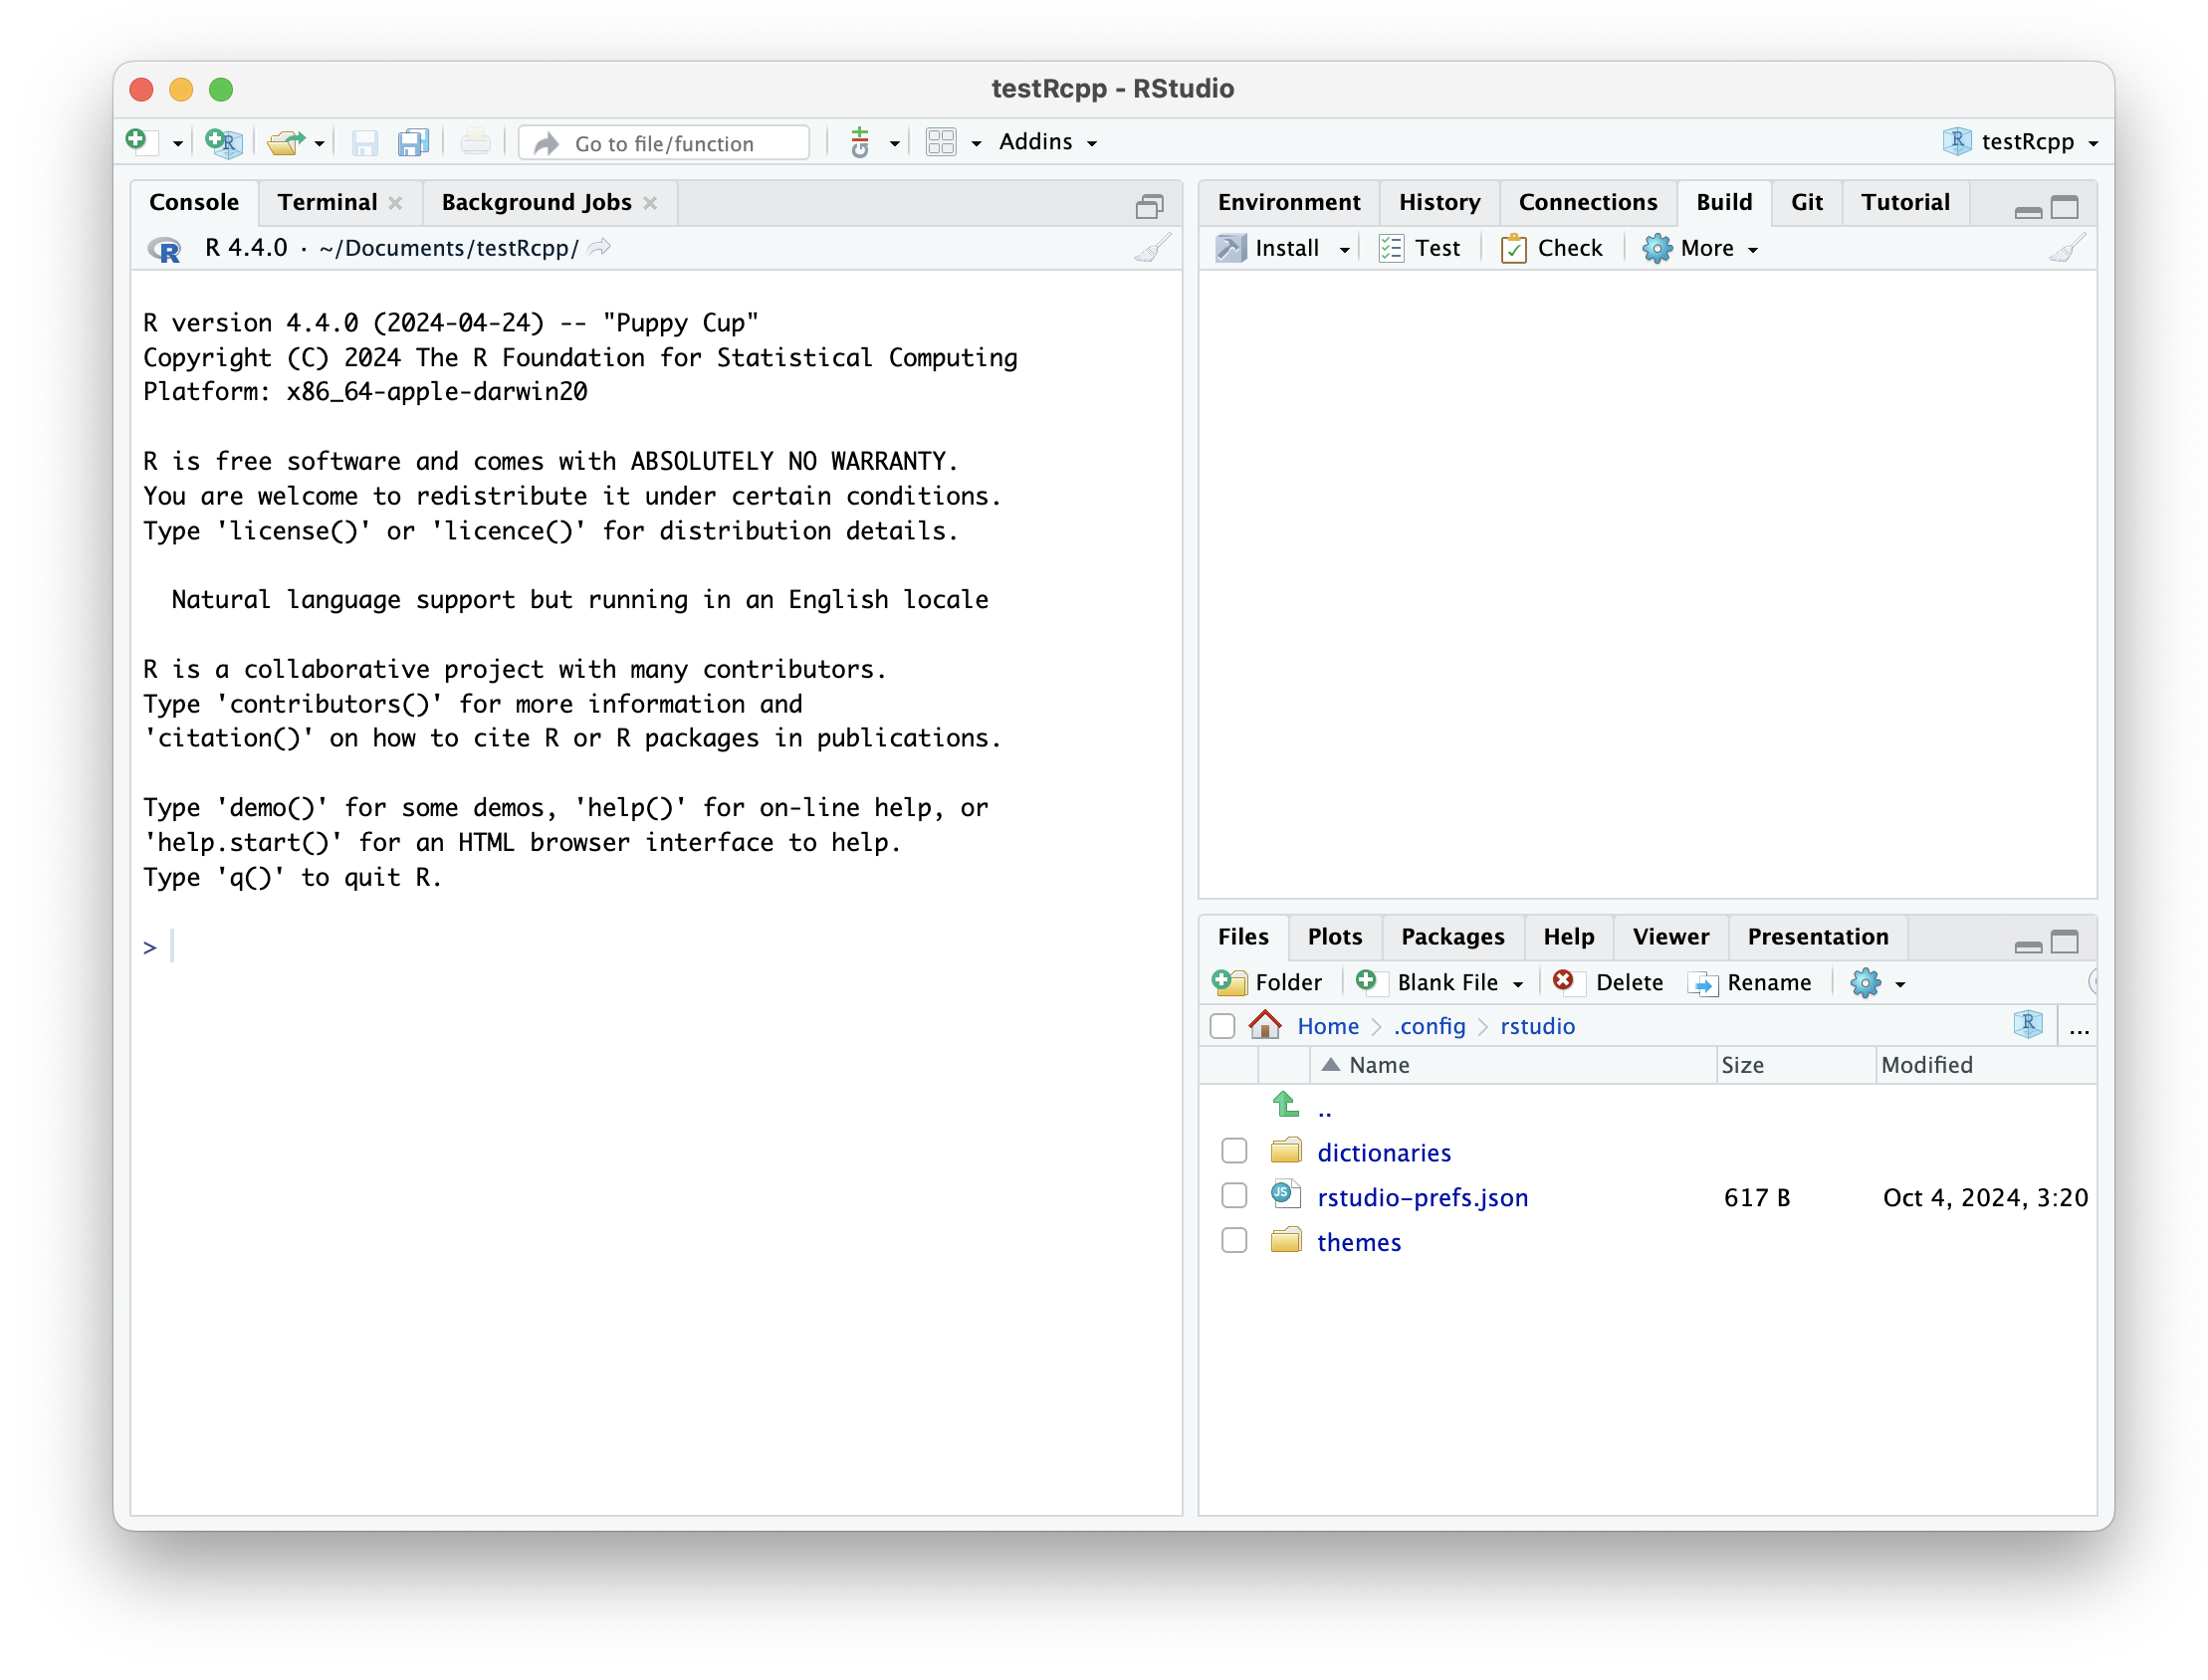
\includegraphics[width=1\textwidth,height=\textheight]{images/main.png}

Nastavení duhových závorek

\begin{figure}

{\centering 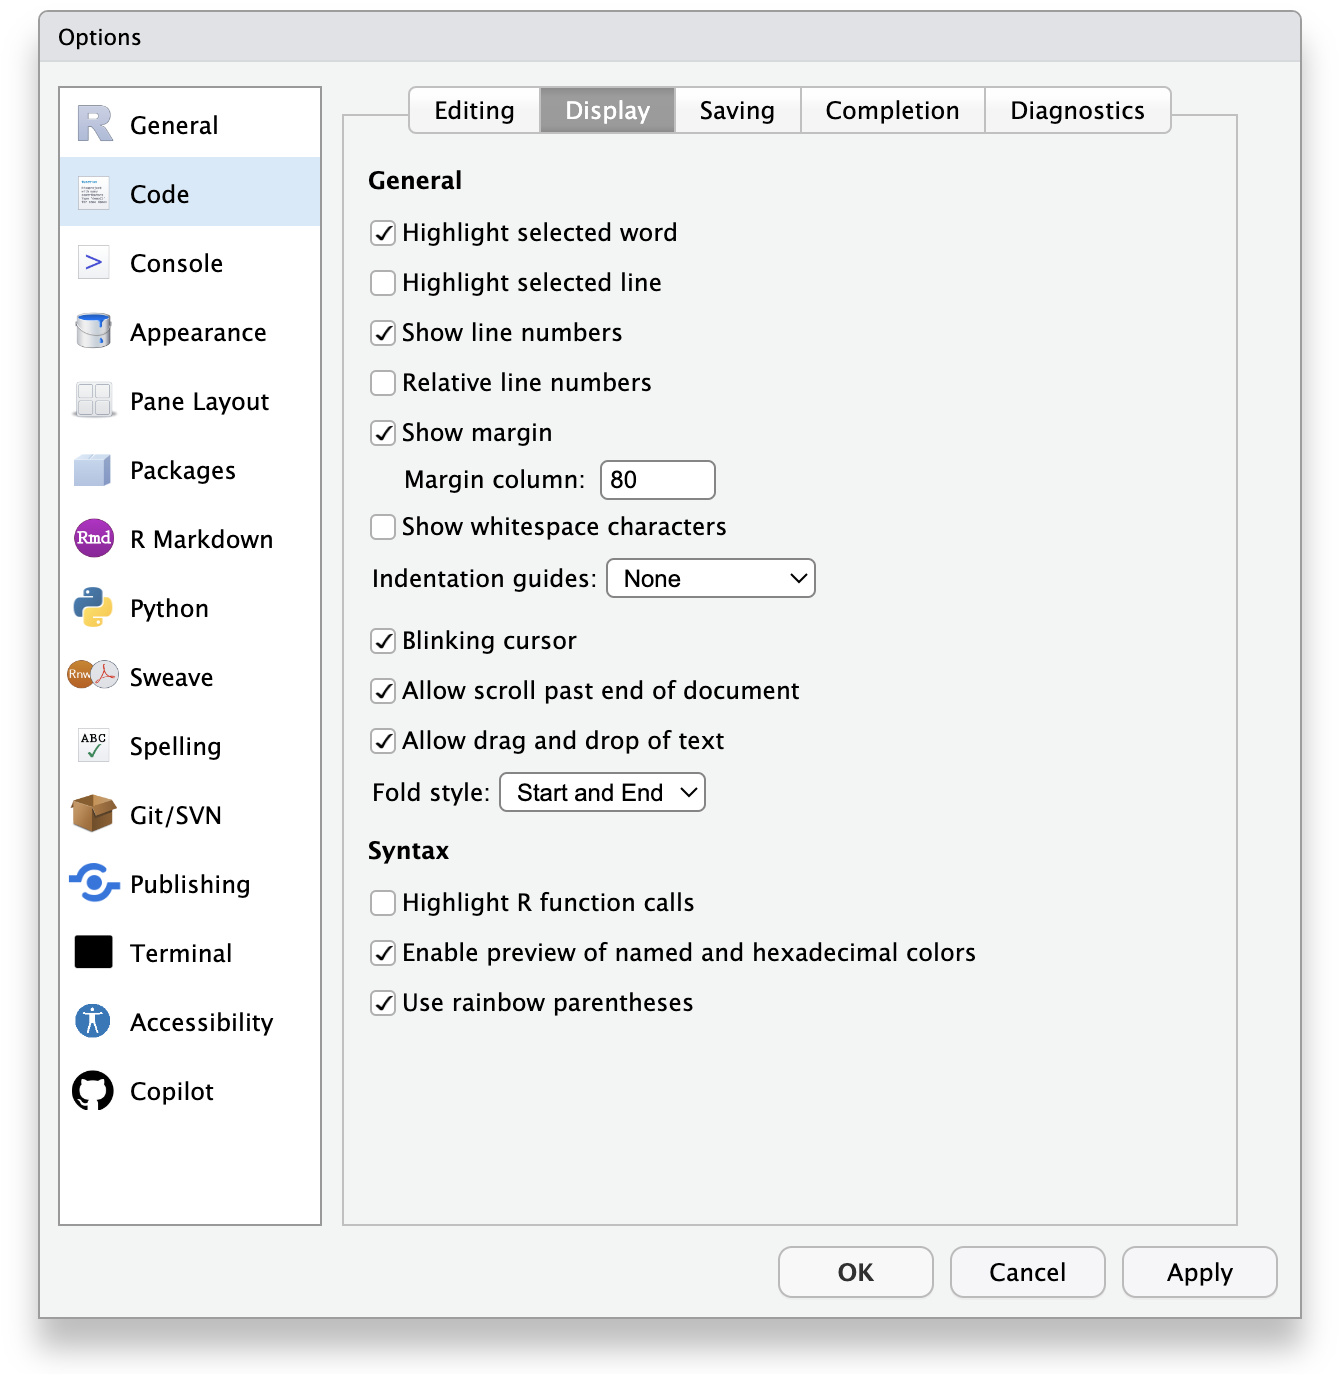
\includegraphics[width=5.3125in,height=\textheight]{images/rainbow-parentheses.png}

}

\caption{Obr. 1}

\end{figure}

\hypertarget{zakluxe1duxe1me-projekt}{%
\section{Zakládáme projekt}\label{zakluxe1duxe1me-projekt}}

Je vhodné seskupovat svoji práci do zv. projektů - ucelených souborů
skriptů, dat a výstupů - podle jednotlivých projektů, kterým se věnuji.

\begin{enumerate}
\def\labelenumi{\arabic{enumi}.}
\item
  Při spuštěném programu z hlavní nabídky vybereme \emph{\textbf{File}
  \textgreater{} \textbf{New Project\ldots{}}}

  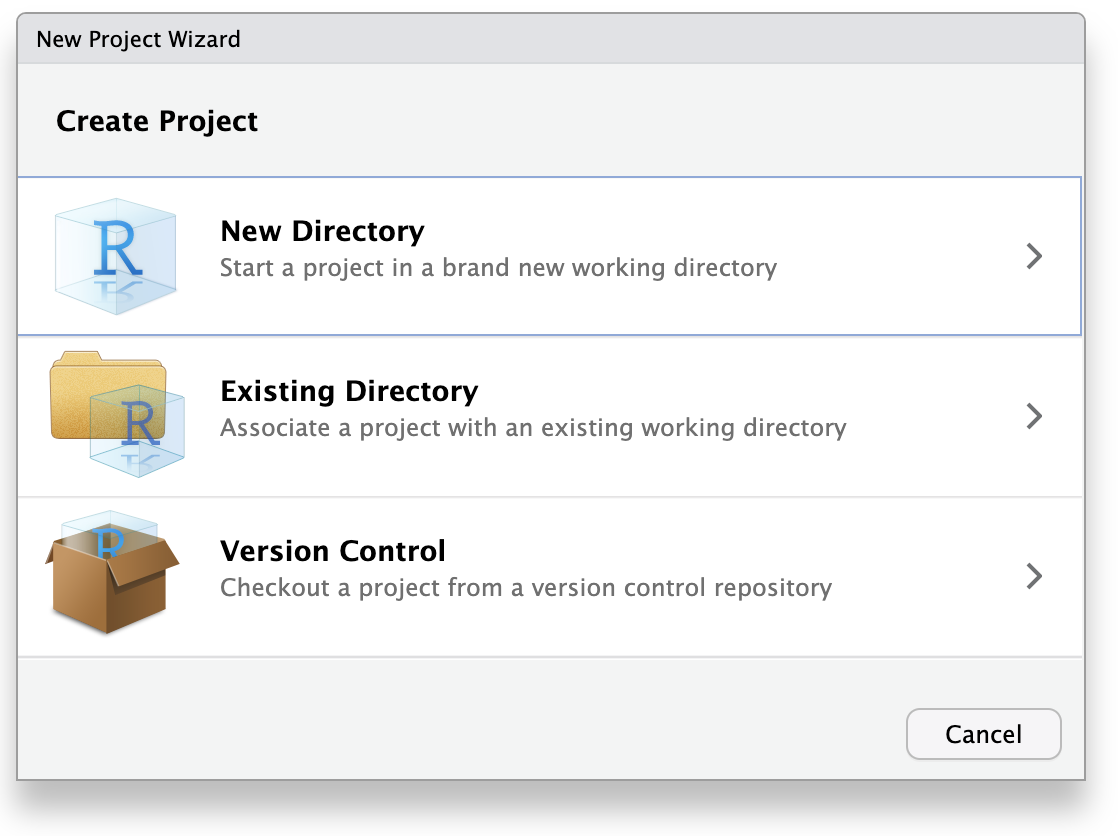
\includegraphics[width=4.69792in,height=\textheight]{images/new_project.png}
\item
  Vybereme \textbf{\emph{New Directory}} a zvolíme \textbf{\emph{New
  Project}}. Ostatní možnosti v tomto kurzu využívate nebudeme.

  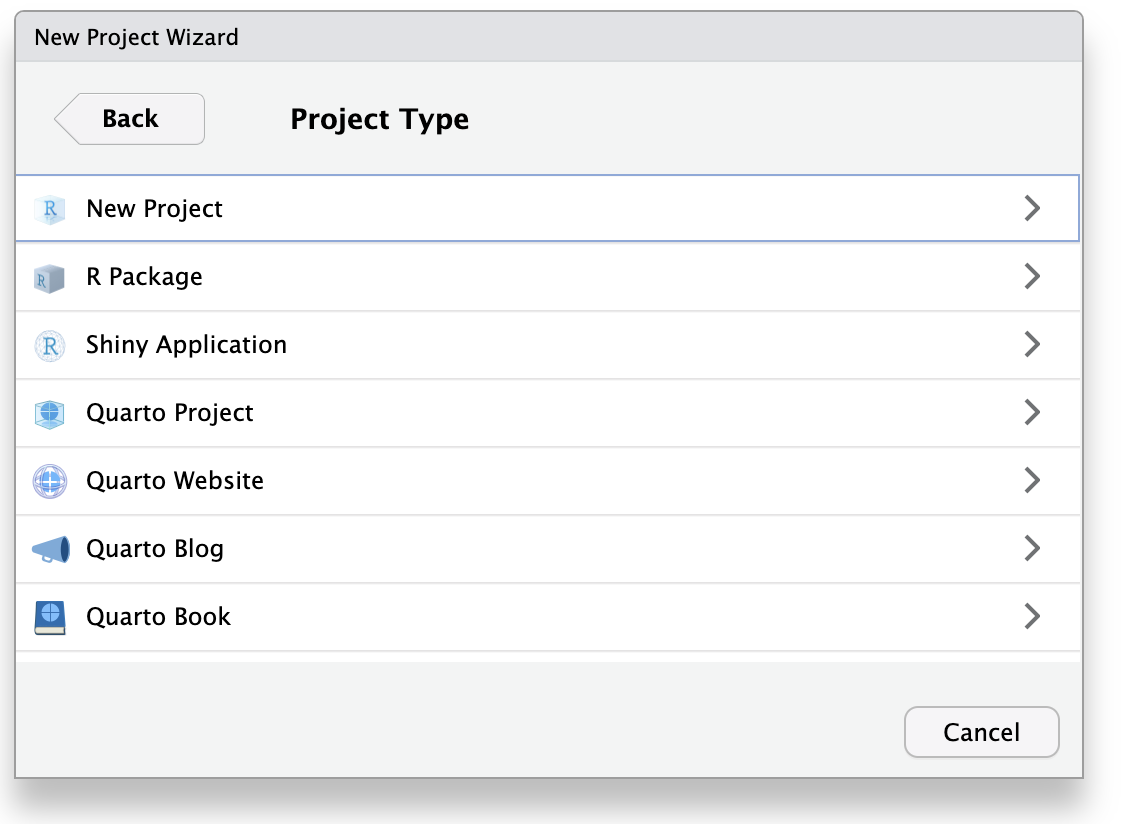
\includegraphics[width=4.78125in,height=\textheight]{images/new_directory.png}
\item
  Projektu je dále nutné zadat název \textbf{\emph{Directory name}}.
  Pokud používate verzovací systém Git, můžete zaškrtnout volbu
  \textbf{\emph{Create a git repository}}. V tomto kurzu používat
  nebudeme.

  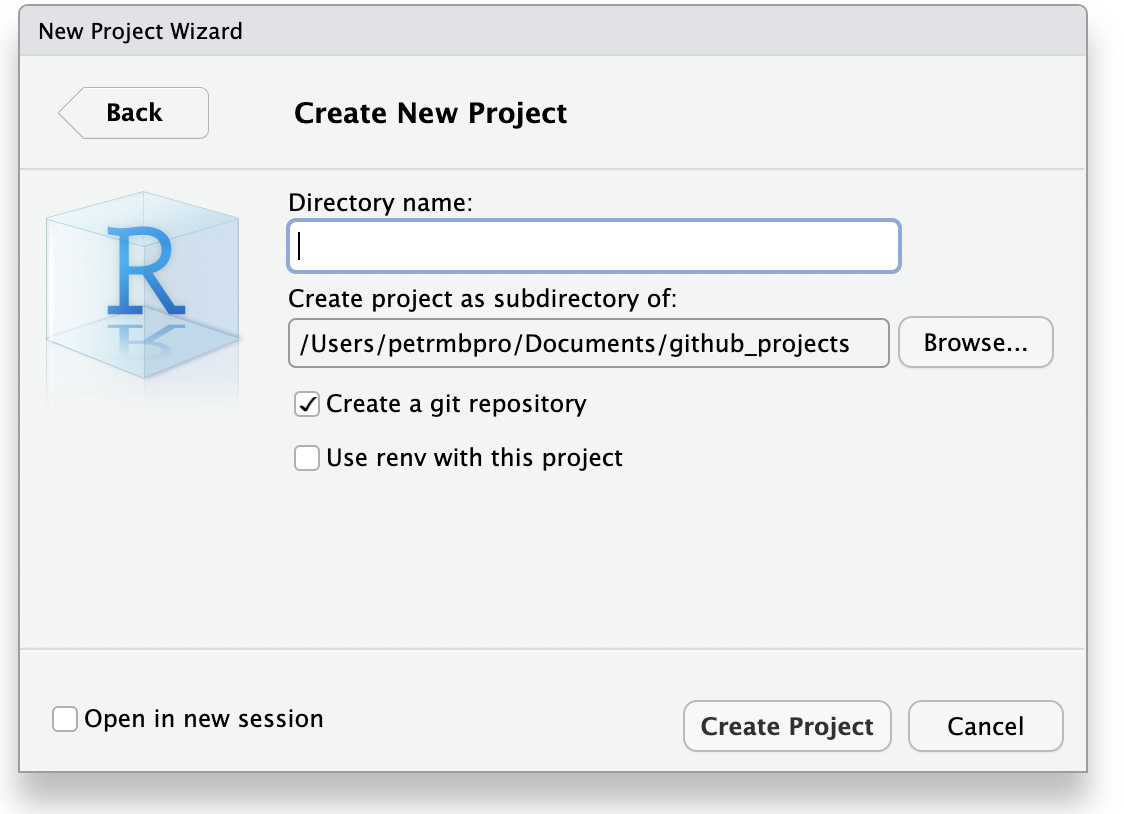
\includegraphics[width=4.76042in,height=\textheight]{images/new_project_name.png}
\item
  Po úspěšném založení projektu by se mělo zobrazit hlavní okno programu
  s přednastvenými panely. V nastavení učeben ČZU odpovídá rozvržení 1.
  obrázku.
\end{enumerate}

\hypertarget{hlavnuxed-okna-a-panely}{%
\section{Hlavní okna a panely}\label{hlavnuxed-okna-a-panely}}

\bookmarksetup{startatroot}

\hypertarget{opakovanuxed-r}{%
\chapter{Opakovaní R}\label{opakovanuxed-r}}

Kurz MVVD navazuje na kurz ``Výpočetní metody'', který je vyučován v
prvním semestru studia Vodního hospodářství. Opakování znalostí jazyka R
jsou věnovány dvě celá úvodní cvičení.

\hypertarget{nuxe1povux11bda}{%
\section{Nápověda}\label{nuxe1povux11bda}}

Zadává se do konzole ve tvaru
\texttt{help(\textless{}jméno\ funkce\textgreater{})}, nebo
\texttt{\textless{}jmeno\ funkce\textgreater{}}. Pokud bychom se chtěli
podívat přímo do kódu funkce, také je to možné, jméno funkce pouze
vepíšeme do konzole bez závorek, případně použijeme příkazu
\texttt{View(jmeno\ funkce)}. Kromě toho existuje v R také
\texttt{help.search(\textless{}jméno\ funkce\textgreater{})} funkce pod
zkratkou \texttt{??}, což vyvolá tématickou nápovědu k již
nainstalovaným funkcím. je ještě možné prohledat mailing list jazyka R
pomocí funkce \texttt{RSiteSearch()}, která otevře nové okno
předdefinovaného prohlížeče. Připravená témata nápovědy:
\texttt{?Logical}, \texttt{?Constants}, \texttt{?Control},
\texttt{?Arithmetic}, \texttt{?Syntax}.

\hypertarget{jmennuxe9-konvence}{%
\section{Jmenné konvence}\label{jmennuxe9-konvence}}

Objekty, které vznikají při práci s R musí splňovat následující jmenné
konvence.- na začátku názvu není číslovka, - název se neshoduje s, či
neobsahuje klíčové slovo.

\hypertarget{kluxedux10dovuxe1-slova}{%
\paragraph*{Klíčová slova}\label{kluxedux10dovuxe1-slova}}
\addcontentsline{toc}{paragraph}{Klíčová slova}

\texttt{if}, \texttt{else}, \texttt{repeat}, \texttt{while},
\texttt{function}, \texttt{for}, \texttt{in}, \texttt{next},
\texttt{repeat}, \texttt{break}, \texttt{TRUE}, \texttt{FALSE},
\texttt{NULL}, \texttt{Inf}, \texttt{NaN}, \texttt{NA},
\texttt{NA\_integer\_}, \texttt{NA\_real\_}, \texttt{NA\_complex\_},
\texttt{NA\_character\_}, a speciální znak: \texttt{\_}

Dále se nedoporučuje vkládat do názvu proměnné tečku ., např. ``.

\hypertarget{pux159uxedklady-nevhodnuxfdch-promux11bnnuxfdch}{%
\paragraph*{Příklady nevhodných
proměnných}\label{pux159uxedklady-nevhodnuxfdch-promux11bnnuxfdch}}
\addcontentsline{toc}{paragraph}{Příklady nevhodných proměnných}

\texttt{aaa}, \texttt{Morávka\ průtok\ {[}m/s{]}},
\texttt{moje.proměnná}

\hypertarget{uvozovky-a-zuxe1vorky}{%
\section{Uvozovky a závorky}\label{uvozovky-a-zuxe1vorky}}

Představují párové znaky jazyka R. Závorky se používají trojího typu:
kulaté, hranaté a složené a všechny mají jasně vymezné pole působnosti.

\begin{enumerate}
\def\labelenumi{\arabic{enumi}.}
\tightlist
\item
  \texttt{(} se používají vždy se jménem funkce a uvozují prostor ve
  kterém se parametrizují argumenty funkce.\\
\item
  \texttt{{[}} se pojí vždy se jménem objektu - vektoru, pole, listu,
  \ldots{} a vymezují výběr z daného objektu.\\
\item
  \texttt{\{} ohraničují blok kódu, který se má vykonat v celku.\\
\end{enumerate}

Není nutné rozlišovat mezi dvojitými '' a jednoduchými ' uvozovkami.
Obojí se dají využívat zástupně. Vždy je nicméně nutné uvozovky správně
spárovat, párované jsou .

\hypertarget{aritmetickuxe9-operace}{%
\section{Aritmetické operace}\label{aritmetickuxe9-operace}}

\hypertarget{annotated-cell-3}{%
\label{annotated-cell-3}}%
\begin{Shaded}
\begin{Highlighting}[]
\DecValTok{1} \SpecialCharTok{+} \DecValTok{1}          \hspace*{\fill}\NormalTok{\circled{1}}
\DecValTok{2} \SpecialCharTok{{-}} \DecValTok{1}          \hspace*{\fill}\NormalTok{\circled{2}}
\DecValTok{1} \SpecialCharTok{*} \FloatTok{3.}         \hspace*{\fill}\NormalTok{\circled{3}}
\DecValTok{1} \SpecialCharTok{*}\NormalTok{ (}\SpecialCharTok{{-}}\DecValTok{1}\NormalTok{)       }
\DecValTok{1} \SpecialCharTok{/} \DecValTok{6}         \hspace*{\fill}\NormalTok{\circled{4}}
\DecValTok{10} \SpecialCharTok{\%\%} \DecValTok{3}       \hspace*{\fill}\NormalTok{\circled{5}}
\DecValTok{7} \SpecialCharTok{\%/\%} \DecValTok{3}        \hspace*{\fill}\NormalTok{\circled{6}}
\DecValTok{10} \SpecialCharTok{**} \DecValTok{3}        \hspace*{\fill}\NormalTok{\circled{7}}
\DecValTok{10} \SpecialCharTok{\%*\%} \DecValTok{3}       \hspace*{\fill}\NormalTok{\circled{8}}
\FunctionTok{sum}\NormalTok{(}\DecValTok{1}\SpecialCharTok{:}\DecValTok{10}\NormalTok{)      }\hspace*{\fill}\NormalTok{\circled{9}}
\FunctionTok{prod}\NormalTok{(}\DecValTok{1}\SpecialCharTok{:}\DecValTok{10}\NormalTok{)     }\hspace*{\fill}\NormalTok{\circled{10}}
\FunctionTok{cumsum}\NormalTok{(}\DecValTok{1}\SpecialCharTok{:}\DecValTok{10}\NormalTok{)   }\hspace*{\fill}\NormalTok{\circled{11}}
\FunctionTok{cumprod}\NormalTok{(}\DecValTok{1}\SpecialCharTok{:}\DecValTok{10}\NormalTok{)  }\hspace*{\fill}\NormalTok{\circled{12}}
\end{Highlighting}
\end{Shaded}

\begin{description}
\tightlist
\item[\circled{1}]
Sčítání
\item[\circled{2}]
Odečítání
\item[\circled{3}]
Násobení
\item[\circled{4}]
Dělení
\item[\circled{5}]
Modulo
\item[\circled{6}]
Celočíselné dělení
\item[\circled{7}]
Mocninné operace
\item[\circled{8}]
Maticové násoobení
\item[\circled{9}]
\(\sum\) prvků z rozsahu
\item[\circled{1}0]
\(\Pi\) prvků z rozsahu
\item[\circled{1}1]
Kumulativní součet prvků z rozsahu
\item[\circled{1}2]
Kumulativní produkt prvků z rozsahu
\end{description}

\hypertarget{operuxe1tory}{%
\section{Operátory}\label{operuxe1tory}}

Kromě aritmetických operátorů, zmíněných
\textbf{?@sec-aritmeticke-operace}

\hypertarget{annotated-cell-4}{%
\label{annotated-cell-4}}%
\begin{Shaded}
\begin{Highlighting}[]
\SpecialCharTok{\textless{}}        \hspace*{\fill}\NormalTok{\circled{1}}
\ErrorTok{\textgreater{}}        \hspace*{\fill}\NormalTok{\circled{2}}
\ErrorTok{\textgreater{}=}       \hspace*{\fill}\NormalTok{\circled{3}}
\ErrorTok{\textless{}=}       \hspace*{\fill}\NormalTok{\circled{4}}
\ErrorTok{==}       \hspace*{\fill}\NormalTok{\circled{5}}
\ErrorTok{!=}       \hspace*{\fill}\NormalTok{\circled{6}}
\ErrorTok{\&}        \hspace*{\fill}\NormalTok{\circled{7}}
\ErrorTok{\&\&}       \hspace*{\fill}\NormalTok{\circled{8}}
\ErrorTok{|}        \hspace*{\fill}\NormalTok{\circled{9}}
\ErrorTok{||}       \hspace*{\fill}\NormalTok{\circled{10}}
\FunctionTok{xor}\NormalTok{(x)    }\hspace*{\fill}\NormalTok{\circled{11}}
\FunctionTok{isTRUE}\NormalTok{(x) }\hspace*{\fill}\NormalTok{\circled{12}}
\FunctionTok{any}\NormalTok{() }\hspace*{\fill}\NormalTok{\circled{13}}
\FunctionTok{all}\NormalTok{() }\hspace*{\fill}\NormalTok{\circled{14}}
\SpecialCharTok{\%in\%} \hspace*{\fill}\NormalTok{\circled{15}}
\FunctionTok{setdiff}\NormalTok{(x, y)  }\hspace*{\fill}\NormalTok{\circled{16}}
\end{Highlighting}
\end{Shaded}

\begin{description}
\tightlist
\item[\circled{1}]
Menší než
\item[\circled{2}]
Větší než
\item[\circled{3}]
Větší nebo rovno
\item[\circled{4}]
Menší nebo rovno
\item[\circled{5}]
Rovno
\item[\circled{6}]
Nerovno
\item[\circled{7}]
Logické ``a''
\item[\circled{8}]
Logické ``a'' přes vektor
\item[\circled{9}]
Logické ``nebo''\\
\item[\circled{1}0]
Logické ``nebo'' přes vektor
\item[\circled{1}1]
Negace
\item[\circled{1}2]
Je \(x\) ``pravda''?
\item[\circled{1}3]
Je něco z obsahu ``pravda''?
\item[\circled{1}4]
Je vše z obsahu ``pravda''?
\item[\circled{1}5]
Je něco obsaženo v?
\item[\circled{1}6]
Chybí něco něco z obsahu v?
\end{description}

\hypertarget{zuxe1kladnuxed-datovuxe9-struktury}{%
\section{Základní datové
struktury}\label{zuxe1kladnuxed-datovuxe9-struktury}}

Základní datové struktury rozlišujeme na atomické (homogenní) a
heterogenní datové struktury.

\hypertarget{homogennuxed-datovuxe9-struktury}{%
\subsection{Homogenní datové
struktury}\label{homogennuxed-datovuxe9-struktury}}

Homogenní datové struktury obsahují atomické vektory, faktory, matice a
pole. Název je odvozen od jejich omezení v podvýběru obsahovat pouze typ
sebe sama tzn. podvýběr matice může být opět pouze matice.

\hypertarget{vektor-vector}{%
\subsubsection{\texorpdfstring{Vektor
\texttt{vector}}{Vektor vector}}\label{vektor-vector}}

Vektor je v jazyce R základní stavební strukturou. Může nabývat
jakéhokoliv datového typu, nicméně všechny prvky v daném vektoru jsou
právě jednoho typu, čímž rozumíme, že je tato struktura tzv. homogenní.
Vektor je možné vytvořit mnoha způsoby, mezi nejčastější patří funkce
\texttt{vector(mode\ =\ "numeric",\ length\ =\ 10)} a funkce
\texttt{c()}, případně vzniká pomocí opetárorů \texttt{{[}} nebo
\texttt{{[}{[}}.

S vektory se pojí důležité pravidlo - \textbf{recyklace hodnot}.

\hypertarget{annotated-cell-5}{%
\label{annotated-cell-5}}%
\begin{Shaded}
\begin{Highlighting}[]
\NormalTok{v }\OtherTok{\textless{}{-}} \FunctionTok{c}\NormalTok{(}\FloatTok{1.4}\NormalTok{, }\FloatTok{2.0}\NormalTok{, }\FloatTok{6.1}\NormalTok{, }\FloatTok{2.7}\NormalTok{)}
\NormalTok{u }\OtherTok{\textless{}{-}} \FunctionTok{c}\NormalTok{(}\FloatTok{2.0}\NormalTok{, }\FloatTok{1.3}\NormalTok{)}
\NormalTok{u }\SpecialCharTok{+}\NormalTok{ v }\hspace*{\fill}\NormalTok{\circled{1}}
\NormalTok{u }\SpecialCharTok{*}\NormalTok{ v }\hspace*{\fill}\NormalTok{\circled{2}}
\end{Highlighting}
\end{Shaded}

\begin{description}
\tightlist
\item[\circled{1}]
Sčítám vektory přičemž délka jednoho je násobkem délky druhého.
\item[\circled{2}]
Násobím vektory přičemž délka jednoho je násobkem délky druhého.
\end{description}

\begin{verbatim}
[1] 3.4 3.3 8.1 4.0
[1]  2.80  2.60 12.20  3.51
\end{verbatim}

\hypertarget{pruxe1ce-s-vektory}{%
\paragraph*{Práce s vektory}\label{pruxe1ce-s-vektory}}
\addcontentsline{toc}{paragraph}{Práce s vektory}

\hypertarget{annotated-cell-6}{%
\label{annotated-cell-6}}%
\begin{Shaded}
\begin{Highlighting}[]
\NormalTok{x }\OtherTok{\textless{}{-}} \DecValTok{1}\SpecialCharTok{:}\DecValTok{10} \CommentTok{\#\textless{}1\textgreater{}}
\NormalTok{x }\OtherTok{\textless{}{-}} \FunctionTok{seq}\NormalTok{(}\DecValTok{10}\SpecialCharTok{:}\DecValTok{1}\NormalTok{) }\CommentTok{\#\textless{}1\textgreater{}}
\NormalTok{x }\OtherTok{\textless{}{-}} \FunctionTok{vector}\NormalTok{(}\AttributeTok{mode =} \StringTok{"numeric"}\NormalTok{, }\AttributeTok{length =} \DecValTok{10}\NormalTok{) }\CommentTok{\#\textless{}1\textgreater{}}
\NormalTok{x }\OtherTok{\textless{}{-}} \FunctionTok{replicate}\NormalTok{(}\AttributeTok{n =} \DecValTok{10}\NormalTok{, }\AttributeTok{expr =} \FunctionTok{eval}\NormalTok{(}\DecValTok{2}\NormalTok{)) }\CommentTok{\#\textless{}1\textgreater{}}
\NormalTok{x }\OtherTok{\textless{}{-}} \FunctionTok{sample}\NormalTok{(}\AttributeTok{x =} \DecValTok{10}\NormalTok{, }\AttributeTok{size =} \DecValTok{10}\NormalTok{, }\AttributeTok{replace =} \ConstantTok{TRUE}\NormalTok{) }\CommentTok{\#\textless{}1\textgreater{}}
\NormalTok{x }\OtherTok{\textless{}{-}} \FunctionTok{rep}\NormalTok{(}\AttributeTok{x =} \DecValTok{15}\NormalTok{, }\AttributeTok{times =} \DecValTok{2}\NormalTok{) }\CommentTok{\#\textless{}1\textgreater{}}
\end{Highlighting}
\end{Shaded}

\begin{description}
\tightlist
\item[\circled{1}]
Tvorba vektoru \(\boldsymbol{\mathrm{x}}\) různými úkony. Použití
sekvence, repetice, opakování a vzorkování.
\end{description}

\hypertarget{matice-matrix}{%
\subsubsection{\texorpdfstring{Matice
\texttt{matrix}}{Matice matrix}}\label{matice-matrix}}

Rozšířením dimenze vektoru vznikne matice nebo obecně pole.

\begin{Shaded}
\begin{Highlighting}[]
\NormalTok{x }\OtherTok{\textless{}{-}} \FunctionTok{c}\NormalTok{(}\DecValTok{1}\SpecialCharTok{:}\DecValTok{10}\NormalTok{)}
\FunctionTok{dim}\NormalTok{(x) }\OtherTok{\textless{}{-}} \FunctionTok{c}\NormalTok{(}\DecValTok{2}\NormalTok{, }\DecValTok{5}\NormalTok{)}
\NormalTok{x}
\end{Highlighting}
\end{Shaded}

\begin{verbatim}
     [,1] [,2] [,3] [,4] [,5]
[1,]    1    3    5    7    9
[2,]    2    4    6    8   10
\end{verbatim}

\begin{longtable}[]{@{}ll@{}}
\toprule\noalign{}
Funkce & Úkon \\
\midrule\noalign{}
\endhead
\bottomrule\noalign{}
\endlastfoot
\texttt{nrow()}, \texttt{nco()} & počet řádků, sloupců matice \\
\texttt{dim()} & řádky \(\times\) sloupce matice \\
\texttt{det()} & deteminant matice \\
\texttt{eigen()} & vlastní čísla a vlastní vektory matice \\
\end{longtable}

\[
A = 
\begin{bmatrix}
1\\
1\\
1\\
1\\
\end{bmatrix}
\]

\hypertarget{annotated-cell-8}{%
\label{annotated-cell-8}}%
\begin{Shaded}
\begin{Highlighting}[]
\NormalTok{A }\OtherTok{\textless{}{-}} \FunctionTok{matrix}\NormalTok{(}\AttributeTok{data =} \FunctionTok{seq}\NormalTok{(}\AttributeTok{from =} \DecValTok{1}\NormalTok{, }\AttributeTok{to =} \DecValTok{16}\NormalTok{, }\AttributeTok{by =} \DecValTok{2}\NormalTok{), }\AttributeTok{nrow =} \DecValTok{4}\NormalTok{)}
\FunctionTok{str}\NormalTok{(A) }\hspace*{\fill}\NormalTok{\circled{1}}
\FunctionTok{dim}\NormalTok{(A) }\hspace*{\fill}\NormalTok{\circled{2}}
\FunctionTok{svd}\NormalTok{(A) }\hspace*{\fill}\NormalTok{\circled{3}}
\FunctionTok{diag}\NormalTok{(A) }\hspace*{\fill}\NormalTok{\circled{4}}
\CommentTok{\# sweep(x = A, MARGIN = 1, STATS = mean)}
\DocumentationTok{\#\#  num [1:4, 1:2] 1 3 5 7 9 11 13 15}
\DocumentationTok{\#\# [1] 4 2}
\DocumentationTok{\#\# $d}
\DocumentationTok{\#\# [1] 25.930394  2.759471}
\DocumentationTok{\#\# }
\DocumentationTok{\#\# $u}
\DocumentationTok{\#\#            [,1]       [,2]}
\DocumentationTok{\#\# [1,] {-}0.3396065 {-}0.7646355}
\DocumentationTok{\#\# [2,] {-}0.4383147 {-}0.3284512}
\DocumentationTok{\#\# [3,] {-}0.5370229  0.1077330}
\DocumentationTok{\#\# [4,] {-}0.6357311  0.5439173}
\DocumentationTok{\#\# }
\DocumentationTok{\#\# $v}
\DocumentationTok{\#\#            [,1]       [,2]}
\DocumentationTok{\#\# [1,] {-}0.3389761  0.9407950}
\DocumentationTok{\#\# [2,] {-}0.9407950 {-}0.3389761}
\DocumentationTok{\#\# }
\DocumentationTok{\#\# [1]  1 11}
\end{Highlighting}
\end{Shaded}

\begin{description}
\tightlist
\item[\circled{1}]
Struktura objektu
\item[\circled{2}]
Dimenze matice
\item[\circled{3}]
Singulární rozklad
\item[\circled{4}]
Prvky na diagonále matice
\end{description}

\hypertarget{heterogennuxed-datovuxe9-struktury}{%
\subsection{Heterogenní datové
struktury}\label{heterogennuxed-datovuxe9-struktury}}

Za \textbf{heterogenní} struktury se označují ty, které mohou uchovávat
dva a více prvků rozdílného typu současně. Z těch základních to jsou
\texttt{data.frame} a \texttt{list}, dále pak \texttt{S4}, nebo
\texttt{R6} třídy, případně další uživatelem vytvořené struktury.

\hypertarget{datovuxe1-tabulka-data.frame}{%
\subsubsection{\texorpdfstring{Datová tabulka
\texttt{data.frame}}{Datová tabulka data.frame}}\label{datovuxe1-tabulka-data.frame}}

\texttt{data.frame} je de facto vektor stejně dlouhých vektorů, které
kromě toho, že musí být shodné délky, mohou být rozdílného typu.

\begin{Shaded}
\begin{Highlighting}[]
\NormalTok{DF }\OtherTok{\textless{}{-}} \FunctionTok{data.frame}\NormalTok{(}\AttributeTok{name =}\NormalTok{ letters[}\DecValTok{1}\SpecialCharTok{:}\DecValTok{5}\NormalTok{], }
                 \AttributeTok{value =} \FunctionTok{rnorm}\NormalTok{(}\DecValTok{5}\NormalTok{))}
\NormalTok{DF}
\DocumentationTok{\#\#   name       value}
\DocumentationTok{\#\# 1    a  0.23634617}
\DocumentationTok{\#\# 2    b {-}1.87150582}
\DocumentationTok{\#\# 3    c  0.04602008}
\DocumentationTok{\#\# 4    d  0.16369628}
\DocumentationTok{\#\# 5    e {-}0.33861297}
\NormalTok{DF[}\StringTok{"name"}\NormalTok{]        }\CommentTok{\# podvýběr do data.frame}
\DocumentationTok{\#\#   name}
\DocumentationTok{\#\# 1    a}
\DocumentationTok{\#\# 2    b}
\DocumentationTok{\#\# 3    c}
\DocumentationTok{\#\# 4    d}
\DocumentationTok{\#\# 5    e}
\NormalTok{DF[[}\StringTok{"name"}\NormalTok{]]      }\CommentTok{\# podvýběr do vektoru}
\DocumentationTok{\#\# [1] "a" "b" "c" "d" "e"}
\NormalTok{DF[, }\StringTok{"name"}\NormalTok{]      }\CommentTok{\# podvýběr do vektoru}
\DocumentationTok{\#\# [1] "a" "b" "c" "d" "e"}
\end{Highlighting}
\end{Shaded}

Práce uvnitř data.frame

\begin{Shaded}
\begin{Highlighting}[]
\NormalTok{DF }\OtherTok{\textless{}{-}} \FunctionTok{data.frame}\NormalTok{(}
  \AttributeTok{mon =} \FunctionTok{rep}\NormalTok{(month.abb, }
            \AttributeTok{times =} \FunctionTok{c}\NormalTok{(}\DecValTok{31}\NormalTok{, }\DecValTok{28}\NormalTok{, }\DecValTok{31}\NormalTok{, }\DecValTok{30}\NormalTok{, }\DecValTok{31}\NormalTok{, }\DecValTok{30}\NormalTok{, }\DecValTok{31}\NormalTok{, }\DecValTok{31}\NormalTok{, }\DecValTok{30}\NormalTok{, }\DecValTok{31}\NormalTok{, }\DecValTok{30}\NormalTok{, }\DecValTok{31}\NormalTok{)), }
  \AttributeTok{value =} \FunctionTok{rnorm}\NormalTok{(}\DecValTok{365}\NormalTok{), }
  \AttributeTok{yr =} \DecValTok{2001}\NormalTok{)}
\FunctionTok{str}\NormalTok{(DF)}
\DocumentationTok{\#\# \textquotesingle{}data.frame\textquotesingle{}:    365 obs. of  3 variables:}
\DocumentationTok{\#\#  $ mon  : chr  "Jan" "Jan" "Jan" "Jan" ...}
\DocumentationTok{\#\#  $ value: num  1.0542 {-}0.5434 {-}0.0107 1.5965 {-}1.8708 ...}
\DocumentationTok{\#\#  $ yr   : num  2001 2001 2001 2001 2001 ...}
\FunctionTok{names}\NormalTok{(DF)}
\DocumentationTok{\#\# [1] "mon"   "value" "yr"}
\FunctionTok{nrow}\NormalTok{(DF)}
\DocumentationTok{\#\# [1] 365}
\FunctionTok{ncol}\NormalTok{(DF)}
\DocumentationTok{\#\# [1] 3}
\end{Highlighting}
\end{Shaded}

\hypertarget{podmuxednky}{%
\section{Podmínky}\label{podmuxednky}}

\begin{Shaded}
\begin{Highlighting}[]
\NormalTok{A }\OtherTok{\textless{}{-}} \DecValTok{1}
\ControlFlowTok{if}\NormalTok{(A }\SpecialCharTok{\textgreater{}=} \DecValTok{1}\NormalTok{) \{}
  \FunctionTok{cat}\NormalTok{(}\StringTok{"A je větší nebo shodné s 1."}\NormalTok{)}
\NormalTok{\}}
\end{Highlighting}
\end{Shaded}

\begin{verbatim}
A je větší nebo shodné s 1.
\end{verbatim}

\hypertarget{annotated-cell-12}{%
\label{annotated-cell-12}}%
\begin{Shaded}
\begin{Highlighting}[]
\NormalTok{A }\OtherTok{\textless{}{-}} \DecValTok{5}
\ControlFlowTok{if}\NormalTok{(A }\SpecialCharTok{\textgreater{}=} \DecValTok{2}\NormalTok{) \{ }\CommentTok{\#\textless{}1\textgreater{}}
  \FunctionTok{cat}\NormalTok{(}\StringTok{"A je větší nebo shodné s 2."}\NormalTok{) }\CommentTok{\#\textless{}1\textgreater{}}
\NormalTok{\} }\ControlFlowTok{else} \ControlFlowTok{if}\NormalTok{(A }\SpecialCharTok{\textgreater{}} \DecValTok{2}\NormalTok{) \{ }\CommentTok{\#\textless{}1\textgreater{}}
  \FunctionTok{cat}\NormalTok{(}\StringTok{"A je větší než 2."}\NormalTok{) }\CommentTok{\#\textless{}1\textgreater{}}
\NormalTok{\} }\CommentTok{\#\textless{}1\textgreater{}}
\end{Highlighting}
\end{Shaded}

\begin{description}
\tightlist
\item[\circled{1}]
Řetěz podmínek se uzavře \textbf{v momentě, kdy je výraz v závorce
poprvé vyhodnocen jako pravdivý}.
\end{description}

\begin{verbatim}
A je větší nebo shodné s 2.
\end{verbatim}

\hypertarget{cyklus}{%
\section{Cyklus}\label{cyklus}}

\hypertarget{for-z-definovanuxe9ho-rozsahu}{%
\subsection{\texorpdfstring{\texttt{for} z definovaného
rozsahu}{for z definovaného rozsahu}}\label{for-z-definovanuxe9ho-rozsahu}}

\begin{Shaded}
\begin{Highlighting}[]
\ControlFlowTok{for}\NormalTok{(i }\ControlFlowTok{in} \DecValTok{1}\SpecialCharTok{:}\DecValTok{4}\NormalTok{) \{}
  \FunctionTok{cat}\NormalTok{(i, }\StringTok{"}\SpecialCharTok{\textbackslash{}n}\StringTok{"}\NormalTok{)}
\NormalTok{\}}
\end{Highlighting}
\end{Shaded}

\begin{verbatim}
1 
2 
3 
4 
\end{verbatim}

\hypertarget{while-s-pomocuxed-podmuxednky}{%
\subsection{\texorpdfstring{\texttt{while} s pomocí
podmínky}{while s pomocí podmínky}}\label{while-s-pomocuxed-podmuxednky}}

\begin{Shaded}
\begin{Highlighting}[]
\NormalTok{i }\OtherTok{\textless{}{-}} \DecValTok{1}
\ControlFlowTok{while}\NormalTok{(i }\SpecialCharTok{\textless{}} \DecValTok{4}\NormalTok{) \{}
  \FunctionTok{cat}\NormalTok{(i, }\StringTok{"}\SpecialCharTok{\textbackslash{}n}\StringTok{"}\NormalTok{)}
\NormalTok{  i }\OtherTok{\textless{}{-}}\NormalTok{ i }\SpecialCharTok{+} \DecValTok{1}
\NormalTok{\}}
\end{Highlighting}
\end{Shaded}

\begin{verbatim}
1 
2 
3 
\end{verbatim}

\hypertarget{repeat-s-uxfanikovou-sekvencuxed}{%
\subsection{\texorpdfstring{\texttt{repeat} s únikovou
sekvencí}{repeat s únikovou sekvencí}}\label{repeat-s-uxfanikovou-sekvencuxed}}

\begin{Shaded}
\begin{Highlighting}[]
\NormalTok{i }\OtherTok{\textless{}{-}} \DecValTok{1}
\ControlFlowTok{repeat}\NormalTok{(\{}
  \FunctionTok{cat}\NormalTok{(i, }\StringTok{"}\SpecialCharTok{\textbackslash{}n}\StringTok{"}\NormalTok{)}
\NormalTok{  i }\OtherTok{\textless{}{-}}\NormalTok{ i }\SpecialCharTok{+} \DecValTok{1}
  \ControlFlowTok{if}\NormalTok{(i }\SpecialCharTok{\textgreater{}=} \DecValTok{4}\NormalTok{) }\ControlFlowTok{break}
\NormalTok{\})}
\end{Highlighting}
\end{Shaded}

\begin{verbatim}
1 
2 
3 
\end{verbatim}

\begin{tcolorbox}[enhanced jigsaw, toprule=.15mm, breakable, title=\textcolor{quarto-callout-tip-color}{\faLightbulb}\hspace{0.5em}{Cvičení}, colframe=quarto-callout-tip-color-frame, bottomrule=.15mm, left=2mm, leftrule=.75mm, colbacktitle=quarto-callout-tip-color!10!white, colback=white, bottomtitle=1mm, toptitle=1mm, opacityback=0, opacitybacktitle=0.6, arc=.35mm, coltitle=black, rightrule=.15mm, titlerule=0mm]

\begin{enumerate}
\def\labelenumi{\arabic{enumi}.}
\item
  Vyhodnoťte s pomocí R následující výrazy:\\
  a) \(1 + 3 \cdot (2 / 3)\:\mathrm{mod}\:3\)\\
  b) \(\left(\dfrac{2}{35}\right)^{0.5} \cdot 3 \cdot (2 / 3)\)\\
  c) \(\sum\limits_{i = 1}^{53}x_i\)\\
  d) \(\dfrac{-\infty}{0}\), \(\dfrac{-\infty}{\infty}\),
  \(\dfrac{0}{0}\)\\
  e) \(\dfrac{\sin(2.3)}{\cos(\pi)}\)\\
  f) \(20!\)\\
  g) \(\int_{0}^{3\pi} \sin(x) dx\)
\item
  Proveďte:\\
  a) Vytvořte vektor hodnot od \(100\) do \(1\) sestupně, využijte
  nápovědu k funkci \texttt{seq()}.\\
  b) Spočtěte rozdíl, matic \(\boldsymbol{\mathrm{A}}\),
  \(\boldsymbol{\mathrm{B}}\). \[\boldsymbol{\mathrm{A}} = \left(
    \begin{matrix}
    2 & 2 & 5\\
    9 & 2 & 7\\
    1 & 3 & 18\\
    \end{matrix}
    \right),\qquad 
    \boldsymbol{\mathrm{B}} = \left(
    \begin{matrix}
    5 & 4 & 5\\
    -7 & 2 & 4\\
    10 & 1 & 5\\
    \end{matrix}
    \right)
    \]\\
  c) Spočítejte inverzní matici k matici \(\boldsymbol{\mathrm{A}}\).
  Najděte vhodnou funkci s pomocí nápovědy.\\
  d) S pomocí hodnot \texttt{TRUE}/\texttt{FALSE} vytvořte matici
  \(\boldsymbol{\mathrm{M}}(3,3)\), změňte typ prvku na pozici
  \(\boldsymbol{\mathrm{M}}[1, 1]\) na textový řetězec. Ovlivní tato
  změna ostatní prvky v matici?
\end{enumerate}

\end{tcolorbox}

\hypertarget{pruxe1ce-s-daty}{%
\section{Práce s daty}\label{pruxe1ce-s-daty}}

Chybějící záznamy a speciální numerické případy \texttt{NA},
\texttt{NaN}, \texttt{NULL}, \texttt{Inf}, \texttt{-Inf} jsou hodnoty,
které mohou vzniknout například jako výsledek početního úkonu, nebo
špatného importu dat. Výraz \texttt{NA} je tvořen v datovém typu
\texttt{logical}, nejméně náročném na paměť. Jinak je možné specifikovat
chybějící hodnotu ve všech ostatních datových typech \texttt{NA\_real\_}
(odpovídá double), \texttt{NA\_integer\_}, \texttt{NA\_complex\_} a
\texttt{NA\_character\_}, které je vhodné využít zejména při vytváření
datového rámce s přesně zadaným typem sloupců. \texttt{NULL} je
návratová hodnota mnoha funkcí a výrazů, reprezentuje prázdný objekt.
Výsledky \texttt{NaN} a \texttt{±Inf} pochází z aritmetických operací
\(\dfrac{1}{0}\) resp. \(\dfrac{\pm0}{1}\) . \texttt{na.omit()},
\texttt{is.na()}, \texttt{complete.cases()}.

\begin{Shaded}
\begin{Highlighting}[]
\NormalTok{global\_temperatures }\OtherTok{\textless{}{-}} \FunctionTok{read.csv}\NormalTok{(}\AttributeTok{file =} \StringTok{"./data/JonesGlobalT.csv"}\NormalTok{, }\AttributeTok{row.names =} \DecValTok{1}\NormalTok{)}
\FunctionTok{head}\NormalTok{(}\AttributeTok{x =}\NormalTok{ global\_temperatures, }\AttributeTok{n =} \DecValTok{5}\NormalTok{)}
\end{Highlighting}
\end{Shaded}

\begin{verbatim}
  YEAR    JAN    FEB    MAR    APR    MAY    JUN    JUL    AUG    SEP    OCT
1 1850 -0.702 -0.284 -0.732 -0.570 -0.325 -0.213 -0.128 -0.233 -0.444 -0.452
2 1851 -0.303 -0.362 -0.485 -0.445 -0.302 -0.189 -0.215 -0.153 -0.108 -0.063
3 1852 -0.308 -0.477 -0.505 -0.559 -0.209 -0.038 -0.016 -0.195 -0.125 -0.216
4 1853 -0.177 -0.330 -0.318 -0.352 -0.268 -0.179 -0.059 -0.148 -0.409 -0.359
5 1854 -0.360 -0.280 -0.284 -0.349 -0.230 -0.215 -0.228 -0.163 -0.115 -0.188
     NOV    DEC ANNUAL
1 -0.190 -0.268 -0.375
2 -0.030 -0.067 -0.223
3 -0.187  0.083 -0.224
4 -0.256 -0.444 -0.271
5 -0.369 -0.232 -0.246
\end{verbatim}

\hypertarget{annotated-cell-17}{%
\label{annotated-cell-17}}%
\begin{Shaded}
\begin{Highlighting}[]
\NormalTok{global\_temperature\_yr }\OtherTok{\textless{}{-}} \FunctionTok{aggregate}\NormalTok{(}\AttributeTok{x =}\NormalTok{ . }\SpecialCharTok{\textasciitilde{}}\NormalTok{ YEAR, }\hspace*{\fill}\NormalTok{\circled{1}}
                                   \AttributeTok{FUN =}\NormalTok{ mean,  }
                                   \AttributeTok{data =}\NormalTok{ global\_temperatures) }
\FunctionTok{head}\NormalTok{(}\AttributeTok{x =}\NormalTok{ global\_temperature\_yr, }\AttributeTok{n =} \DecValTok{5}\NormalTok{)}
\end{Highlighting}
\end{Shaded}

\begin{description}
\tightlist
\item[\circled{1}]
Agregace dat do průměrů za roční období.
\end{description}

\begin{verbatim}
  YEAR    JAN    FEB    MAR    APR    MAY    JUN    JUL    AUG    SEP    OCT
1 1850 -0.702 -0.284 -0.732 -0.570 -0.325 -0.213 -0.128 -0.233 -0.444 -0.452
2 1851 -0.303 -0.362 -0.485 -0.445 -0.302 -0.189 -0.215 -0.153 -0.108 -0.063
3 1852 -0.308 -0.477 -0.505 -0.559 -0.209 -0.038 -0.016 -0.195 -0.125 -0.216
4 1853 -0.177 -0.330 -0.318 -0.352 -0.268 -0.179 -0.059 -0.148 -0.409 -0.359
5 1854 -0.360 -0.280 -0.284 -0.349 -0.230 -0.215 -0.228 -0.163 -0.115 -0.188
     NOV    DEC ANNUAL
1 -0.190 -0.268 -0.375
2 -0.030 -0.067 -0.223
3 -0.187  0.083 -0.224
4 -0.256 -0.444 -0.271
5 -0.369 -0.232 -0.246
\end{verbatim}

\begin{Shaded}
\begin{Highlighting}[]
\FunctionTok{par}\NormalTok{(}\AttributeTok{mfrow =} \FunctionTok{c}\NormalTok{(}\DecValTok{1}\NormalTok{, }\DecValTok{2}\NormalTok{))}
\FunctionTok{with}\NormalTok{(}\AttributeTok{data =}\NormalTok{ global\_temperature\_yr, }\AttributeTok{expr =} \FunctionTok{plot}\NormalTok{(YEAR, JAN, }\AttributeTok{type =} \StringTok{"l"}\NormalTok{))}
\FunctionTok{with}\NormalTok{(}\AttributeTok{data =}\NormalTok{ global\_temperature\_yr, }
     \AttributeTok{expr =} \FunctionTok{boxplot}\NormalTok{(ANNUAL, }\AttributeTok{horizontal =} \ConstantTok{TRUE}\NormalTok{))}
\end{Highlighting}
\end{Shaded}

\begin{figure}[H]

{\centering 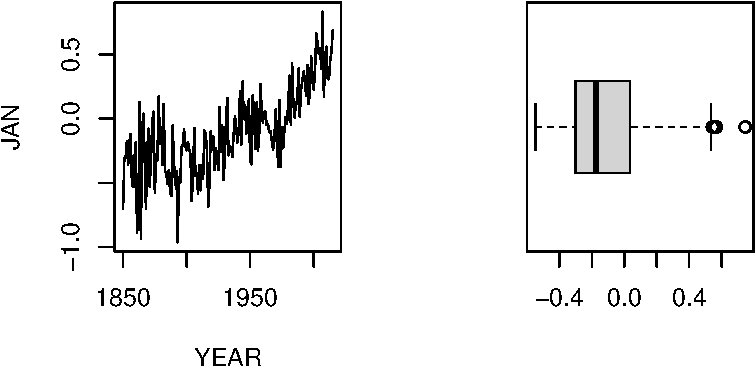
\includegraphics{02_uvod_do_R_2_files/figure-pdf/unnamed-chunk-15-1.pdf}

}

\end{figure}

\begin{tcolorbox}[enhanced jigsaw, toprule=.15mm, breakable, title=\textcolor{quarto-callout-tip-color}{\faLightbulb}\hspace{0.5em}{Cvičení}, colframe=quarto-callout-tip-color-frame, bottomrule=.15mm, left=2mm, leftrule=.75mm, colbacktitle=quarto-callout-tip-color!10!white, colback=white, bottomtitle=1mm, toptitle=1mm, opacityback=0, opacitybacktitle=0.6, arc=.35mm, coltitle=black, rightrule=.15mm, titlerule=0mm]

\begin{enumerate}
\def\labelenumi{\arabic{enumi}.}
\tightlist
\item
  Nahrajte data do prostředí s pomocí vhodně parametrizované
  \texttt{read.\_\_\_()} funkce.\\
\item
  Doplňte hydrologický rok.\\
\item
  Proveďte agregaci dat průměrem pro jednotlivé měsíce.\\
\item
  Vyneste do grafu pomocí funkce \texttt{plot()}.
\end{enumerate}

\end{tcolorbox}

\bookmarksetup{startatroot}

\hypertarget{grafickuxfd-vuxfdstup}{%
\chapter{Grafický výstup}\label{grafickuxfd-vuxfdstup}}

\begin{tcolorbox}[enhanced jigsaw, toprule=.15mm, breakable, title=\textcolor{quarto-callout-warning-color}{\faExclamationTriangle}\hspace{0.5em}{Cíle cvičení}, colframe=quarto-callout-warning-color-frame, bottomrule=.15mm, left=2mm, leftrule=.75mm, colbacktitle=quarto-callout-warning-color!10!white, colback=white, bottomtitle=1mm, toptitle=1mm, opacityback=0, opacitybacktitle=0.6, arc=.35mm, coltitle=black, rightrule=.15mm, titlerule=0mm]

\begin{itemize}
\tightlist
\item
  Naučit se tvorbu základních typů grafů
\item
  Rozdělení sazby výstupu do polí
\end{itemize}

\end{tcolorbox}

Opět připravím datovou sadu, tentokrát umístíme do \texttt{data.frame}
jménem \texttt{dfr}.

\hypertarget{annotated-cell-19}{%
\label{annotated-cell-19}}%
\begin{Shaded}
\begin{Highlighting}[]
\NormalTok{dfr }\OtherTok{\textless{}{-}} \FunctionTok{data.frame}\NormalTok{(}
  \AttributeTok{X =} \DecValTok{1}\SpecialCharTok{:}\DecValTok{100}\NormalTok{,}
  \AttributeTok{Y =} \FunctionTok{rnorm}\NormalTok{(}\DecValTok{100}\NormalTok{) }\hspace*{\fill}\NormalTok{\circled{1}}
\NormalTok{)}
\end{Highlighting}
\end{Shaded}

\begin{description}
\tightlist
\item[\circled{1}]
K vytvoření proměnné \(Y\) použijeme generování čísel z náhodného
rozdělení s parametry \(\mu = 0\) a \(\sigma = 1\); více v kapitole
Kapitola~\ref{sec-rozdeleni}
\end{description}

\hypertarget{funkce-curve}{%
\section{\texorpdfstring{Funkce
\texttt{curve()}}{Funkce curve()}}\label{funkce-curve}}

Curve je funkce, která se uplatní při tvorbě symbolických grafů
matematických funkcí, kdy není třeba parametrizovat argument \texttt{x}.

\begin{Shaded}
\begin{Highlighting}[]
\FunctionTok{curve}\NormalTok{(}\AttributeTok{expr =} \FunctionTok{tanh}\NormalTok{(x),}
      \AttributeTok{from =} \SpecialCharTok{{-}}\NormalTok{pi, }
      \AttributeTok{to =}\NormalTok{ pi)}
\end{Highlighting}
\end{Shaded}

\begin{figure}[H]

{\centering 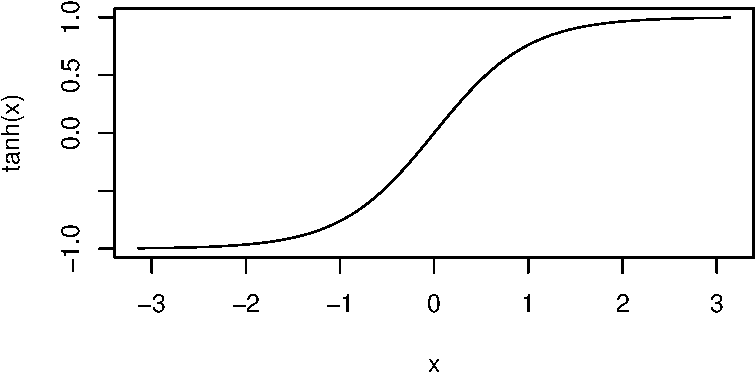
\includegraphics{03_grafy_files/figure-pdf/unnamed-chunk-2-1.pdf}

}

\end{figure}

\hypertarget{funkce-plot}{%
\section{\texorpdfstring{Funkce
\texttt{plot()}}{Funkce plot()}}\label{funkce-plot}}

\texttt{plot(x,\ y,\ ...)} je základní \textbf{S3 generická} funkce,
jejíž metody umožňují použití na široké množství objektů. Začneme s
použitím na vektor z datasetu \texttt{dfr}.

\hypertarget{annotated-cell-21}{%
\label{annotated-cell-21}}%
\begin{Shaded}
\begin{Highlighting}[]
\FunctionTok{plot}\NormalTok{(dfr}\SpecialCharTok{$}\NormalTok{Y) }\hspace*{\fill}\NormalTok{\circled{1}}
\end{Highlighting}
\end{Shaded}

\begin{description}
\tightlist
\item[\circled{1}]
Funkce má věšinu svých argumentů parametrizovaných v přednastavenými
hodnotami, nebo hodnotami novodvozenými od parametru. Vidíme tak, že osa
\(y\) je pojmenována po vstupním parametru. V celém znění funkce vypadá
následovně:\textasciitilde\textasciitilde\textasciitilde{} plot(x, y =
NULL, type = ``p'', xlim = NULL, ylim = NULL, log = ````, main = NULL,
sub = NULL, xlab = NULL, ylab = NULL, ann = par(''ann''), axes = TRUE,
frame.plot = axes, panel.first = NULL, panel.last = NULL, asp = NA,
xgap.axis = NA, ygap.axis = NA, \ldots)
\textasciitilde\textasciitilde\textasciitilde{}
\end{description}

\begin{figure}[H]

{\centering 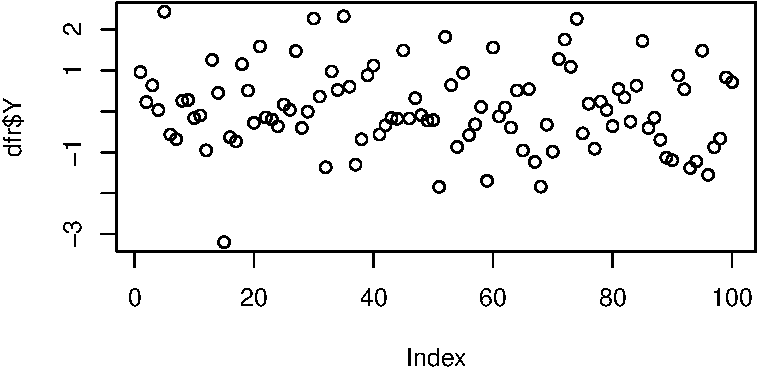
\includegraphics{03_grafy_files/figure-pdf/unnamed-chunk-3-1.pdf}

}

\end{figure}

\hypertarget{annotated-cell-22}{%
\label{annotated-cell-22}}%
\begin{Shaded}
\begin{Highlighting}[]
\FunctionTok{plot}\NormalTok{(}\AttributeTok{x =}\NormalTok{ dfr}\SpecialCharTok{$}\NormalTok{X, }\hspace*{\fill}\NormalTok{\circled{1}}
     \AttributeTok{y =}\NormalTok{ dfr}\SpecialCharTok{$}\NormalTok{Y, }
     \AttributeTok{type =} \StringTok{"b"}\NormalTok{, }\hspace*{\fill}\NormalTok{\circled{2}}
     \AttributeTok{col =} \StringTok{"gray10"}\NormalTok{, }\hspace*{\fill}\NormalTok{\circled{3}}
     \AttributeTok{pch =} \DecValTok{21}\NormalTok{, }\hspace*{\fill}\NormalTok{\circled{4}}
     \AttributeTok{bg =} \StringTok{"\#4a6777"}\NormalTok{, }\hspace*{\fill}\NormalTok{\circled{5}}
     \AttributeTok{ylim =} \FunctionTok{c}\NormalTok{(}\SpecialCharTok{{-}}\FunctionTok{abs}\NormalTok{(}\FloatTok{1.25} \SpecialCharTok{*} \FunctionTok{min}\NormalTok{(dfr}\SpecialCharTok{$}\NormalTok{Y)), }\hspace*{\fill}\NormalTok{\circled{6}}
              \FloatTok{1.25} \SpecialCharTok{*} \FunctionTok{max}\NormalTok{(dfr}\SpecialCharTok{$}\NormalTok{Y)), }
     \AttributeTok{xlab =} \StringTok{""}\NormalTok{, }\hspace*{\fill}\NormalTok{\circled{7}}
     \AttributeTok{ylab =} \StringTok{"Value"}\NormalTok{, }
     \AttributeTok{main =} \StringTok{"Y\textasciitilde{}X vztah"}\NormalTok{,  }\hspace*{\fill}\NormalTok{\circled{8}}
     \AttributeTok{sub =} \FunctionTok{Sys.Date}\NormalTok{()) }\hspace*{\fill}\NormalTok{\circled{9}}
\FunctionTok{legend}\NormalTok{(}\AttributeTok{x =} \StringTok{"topright"}\NormalTok{, }\hspace*{\fill}\NormalTok{\circled{10}}
       \AttributeTok{fill =} \StringTok{"\#4a6777"}\NormalTok{, }\hspace*{\fill}\NormalTok{\circled{11}}
       \AttributeTok{pch =} \DecValTok{21}\NormalTok{, }\hspace*{\fill}\NormalTok{\circled{12}}
       \AttributeTok{legend =} \FunctionTok{c}\NormalTok{(}\StringTok{"Y"}\NormalTok{), }\hspace*{\fill}\NormalTok{\circled{13}}
       \AttributeTok{box.col =} \ConstantTok{NA}\NormalTok{, }\hspace*{\fill}\NormalTok{\circled{14}}
       \AttributeTok{lty =} \DecValTok{1}\NormalTok{, }\hspace*{\fill}\NormalTok{\circled{15}}
       \AttributeTok{col =} \StringTok{"gray10"}\NormalTok{) }\hspace*{\fill}\NormalTok{\circled{16}}
\end{Highlighting}
\end{Shaded}

\begin{description}
\tightlist
\item[\circled{1}]
Základní proměnné \(X\) a \(Y\) pro typ grafu.
\item[\circled{2}]
Volba typu grafu \texttt{"b"} označuje body protnuté spojnicí.
\item[\circled{3}]
Volba barvy popředí znaku bod/přímka.
\item[\circled{4}]
Volba charakteru bodového znaku.
\item[\circled{5}]
Volba barvy pozadí znaku umožňujícího výplň - bod.
\item[\circled{6}]
Změna rozsahu osy \(y\).
\item[\circled{7}]
Změna názvu os.
\item[\circled{8}]
Znění hlavního nadpisu.
\item[\circled{9}]
Podnadpis \emph{dtto}.
\item[\circled{1}0]
Pokračujeme nastavením umístění legendy.
\item[\circled{1}1]
Výplň prvku v legendě.
\item[\circled{1}2]
Typ prvku v legendě.
\item[\circled{1}3]
Název prvku v legendě.
\item[\circled{1}4]
Volba barvy ohraničení legendy
\item[\circled{1}5]
Volba typu spojnice (1 = plná čára)
\item[\circled{1}6]
Volba barvy popředí prvku legendy
\end{description}

\begin{figure}[H]

{\centering 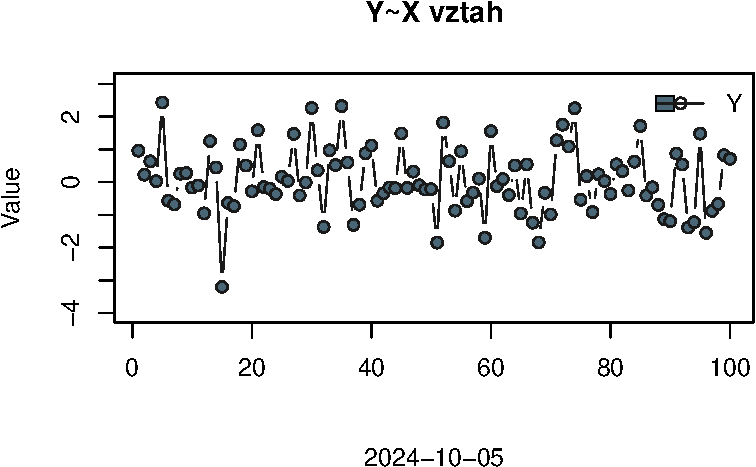
\includegraphics{03_grafy_files/figure-pdf/unnamed-chunk-4-1.pdf}

}

\end{figure}

\hypertarget{annotated-cell-23}{%
\label{annotated-cell-23}}%
\begin{Shaded}
\begin{Highlighting}[]
\FunctionTok{with}\NormalTok{(}\AttributeTok{data =}\NormalTok{ dfr, }\hspace*{\fill}\NormalTok{\circled{1}}
     \AttributeTok{expr =}\NormalTok{ \{ }\hspace*{\fill}\NormalTok{\circled{2}}
       \FunctionTok{plot}\NormalTok{(}\AttributeTok{x =}\NormalTok{ X, }\AttributeTok{y =}\NormalTok{ Y)  }
       \FunctionTok{lines}\NormalTok{(}\AttributeTok{x =}\NormalTok{ X, }\AttributeTok{y =}\NormalTok{ Y) }
\NormalTok{       \}}
\NormalTok{     ) }
\end{Highlighting}
\end{Shaded}

\begin{description}
\tightlist
\item[\circled{1}]
Funkce \texttt{with()} umožňuje zavolání funkce uvedené v arugmentu
\texttt{expr} na proměnných v \texttt{data.frame}. Odpadá opakované
psaní prefixu datové sady (zde \texttt{dfr\$\_\_\_})
\item[\circled{2}]
Argument \texttt{expr} může obsahovat i blok kódu \texttt{\{...\}}
\end{description}

\begin{figure}[H]

{\centering 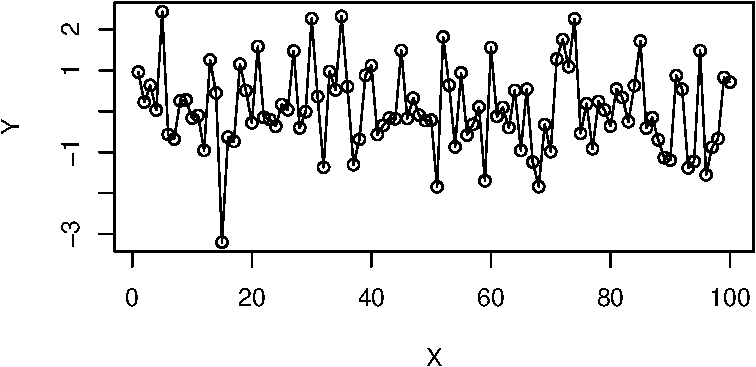
\includegraphics{03_grafy_files/figure-pdf/unnamed-chunk-5-1.pdf}

}

\end{figure}

\hypertarget{volba-barev}{%
\section{Volba barev}\label{volba-barev}}

Výpis všech předdefinovaných barev\footnote{Předdefinovaných barev je
  celkem 657.} lze získat příkazem \texttt{colors()}.

\begin{Shaded}
\begin{Highlighting}[]
\FunctionTok{colors}\NormalTok{()[}\DecValTok{1}\SpecialCharTok{:}\DecValTok{10}\NormalTok{]}
\end{Highlighting}
\end{Shaded}

\begin{verbatim}
 [1] "white"         "aliceblue"     "antiquewhite"  "antiquewhite1"
 [5] "antiquewhite2" "antiquewhite3" "antiquewhite4" "aquamarine"   
 [9] "aquamarine1"   "aquamarine2"  
\end{verbatim}

\hypertarget{vytvuxe1ux159uxedme-layout}{%
\section{Vytváříme layout}\label{vytvuxe1ux159uxedme-layout}}

Jednoduchý pravidelný layout můžeme vytvořit změnou parametrů okna
grafického výstupu pomocí funkce \texttt{par()}

\hypertarget{sazba-pomocuxed-par}{%
\subsection{\texorpdfstring{Sazba pomocí
\texttt{par()}}{Sazba pomocí par()}}\label{sazba-pomocuxed-par}}

\hypertarget{annotated-cell-25}{%
\label{annotated-cell-25}}%
\begin{Shaded}
\begin{Highlighting}[]
\FunctionTok{par}\NormalTok{(}\AttributeTok{mfrow =} \FunctionTok{c}\NormalTok{(}\DecValTok{1}\NormalTok{, }\DecValTok{2}\NormalTok{)) }\CommentTok{\#\textless{}1\textgreater{}}
\FunctionTok{hist}\NormalTok{(dfr}\SpecialCharTok{$}\NormalTok{X, }\AttributeTok{main =} \StringTok{"X"}\NormalTok{, }\AttributeTok{xlab =} \StringTok{""}\NormalTok{) }\hspace*{\fill}\NormalTok{\circled{2}}
\FunctionTok{hist}\NormalTok{(dfr}\SpecialCharTok{$}\NormalTok{Y, }\AttributeTok{main =} \StringTok{"Y"}\NormalTok{, }\AttributeTok{xlab =} \StringTok{""}\NormalTok{) }
\end{Highlighting}
\end{Shaded}

\begin{description}
\tightlist
\item[\circled{1}]
Okno výstupu rozdělíme do dvou sloupců na jednom řádku.
\item[\circled{2}]
Posléze voláme dva grafy, které postupně vyplní pole v daném okně.
\end{description}

\begin{figure}[H]

{\centering 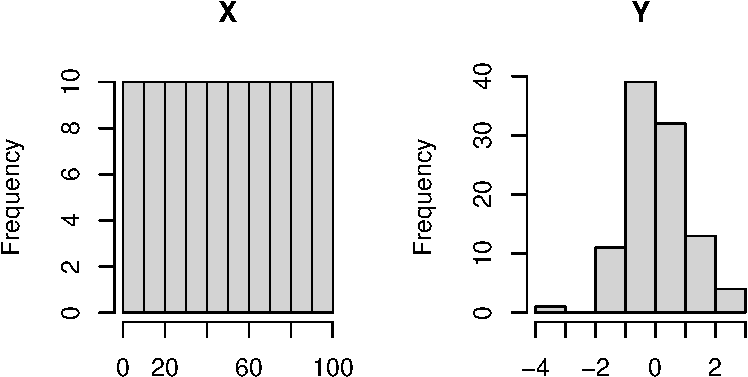
\includegraphics{03_grafy_files/figure-pdf/unnamed-chunk-7-1.pdf}

}

\end{figure}

\hypertarget{sazba-s-funkcuxed-layout-a-matice}{%
\subsection{\texorpdfstring{Sazba s funkcí \texttt{layout()} a
matice}{Sazba s funkcí layout() a matice}}\label{sazba-s-funkcuxed-layout-a-matice}}

\begin{Shaded}
\begin{Highlighting}[]
\FunctionTok{layout.show}\NormalTok{(}
  \FunctionTok{layout}\NormalTok{(}
    \AttributeTok{mat =} \FunctionTok{matrix}\NormalTok{(}
      \AttributeTok{data =} \FunctionTok{c}\NormalTok{(}\DecValTok{2}\NormalTok{, }\DecValTok{2}\NormalTok{, }\DecValTok{0}\NormalTok{,}
               \DecValTok{1}\NormalTok{, }\DecValTok{1}\NormalTok{, }\DecValTok{3}\NormalTok{,}
               \DecValTok{1}\NormalTok{, }\DecValTok{1}\NormalTok{, }\DecValTok{3}\NormalTok{), }
      \AttributeTok{nrow =} \DecValTok{3}\NormalTok{, }
      \AttributeTok{ncol =} \DecValTok{3}\NormalTok{, }
      \AttributeTok{byrow =} \ConstantTok{TRUE}\NormalTok{)))}
\end{Highlighting}
\end{Shaded}

\begin{figure}[H]

{\centering 
\includegraphics{03_grafy_files/figure-pdf/unnamed-chunk-8-1.pdf}

}

\end{figure}

\bookmarksetup{startatroot}

\hypertarget{popisnuxe1-statistika}{%
\chapter{Popisná statistika}\label{popisnuxe1-statistika}}

Funkce pro statistické zpracování datového souboru nalezneme v balíčku
\texttt{stats}, jehož jmenný prostor je připojen po otevření R.\\

Popisná statistika má za cíle \textbf{souhrnně popsat soubor} (spíše než
použít data k získání informací o populaci, o které se předpokládá, že
vzorek dat reprezentuje).

\begin{tcolorbox}[enhanced jigsaw, toprule=.15mm, breakable, title=\textcolor{quarto-callout-warning-color}{\faExclamationTriangle}\hspace{0.5em}{Cíle cvičení}, colframe=quarto-callout-warning-color-frame, bottomrule=.15mm, left=2mm, leftrule=.75mm, colbacktitle=quarto-callout-warning-color!10!white, colback=white, bottomtitle=1mm, toptitle=1mm, opacityback=0, opacitybacktitle=0.6, arc=.35mm, coltitle=black, rightrule=.15mm, titlerule=0mm]

\begin{itemize}
\tightlist
\item
  Být schopen popsat číselné proměnné v datech popsat s pomocí uvedených
  statistik\\
\end{itemize}

\end{tcolorbox}

Níže uvedené funkce jsou počítané s pomocí následujícího vektoru

\begin{Shaded}
\begin{Highlighting}[]
\FunctionTok{set.seed}\NormalTok{(}\DecValTok{1}\NormalTok{)}
\NormalTok{x }\OtherTok{\textless{}{-}} \FunctionTok{round}\NormalTok{(}\FunctionTok{rnorm}\NormalTok{(}\DecValTok{30}\NormalTok{), }\DecValTok{2}\NormalTok{)}
\NormalTok{x}
\DocumentationTok{\#\#  [1] {-}0.63  0.18 {-}0.84  1.60  0.33 {-}0.82  0.49  0.74  0.58 {-}0.31  1.51  0.39}
\DocumentationTok{\#\# [13] {-}0.62 {-}2.21  1.12 {-}0.04 {-}0.02  0.94  0.82  0.59  0.92  0.78  0.07 {-}1.99}
\DocumentationTok{\#\# [25]  0.62 {-}0.06 {-}0.16 {-}1.47 {-}0.48  0.42}
\end{Highlighting}
\end{Shaded}

\hypertarget{muxedry-polohy}{%
\section{Míry polohy}\label{muxedry-polohy}}

\hypertarget{minimum-maximum}{%
\subsection{Minimum, maximum}\label{minimum-maximum}}

Pro oba extrémy jsou v R stejnojmenné funkce.

\[
 \max(x)\\
 \min(x)\\
 \min(x) - \max(x)
\]\\

\hypertarget{vuxfdbux11brovuxfd-kvantil}{%
\subsection{Výběrový kvantil}\label{vuxfdbux11brovuxfd-kvantil}}

\hypertarget{annotated-cell-28}{%
\label{annotated-cell-28}}%
\begin{Shaded}
\begin{Highlighting}[]
\FunctionTok{t}\NormalTok{(}\FunctionTok{sapply}\NormalTok{(}\AttributeTok{X =} \DecValTok{1}\SpecialCharTok{:}\DecValTok{7}\NormalTok{, }\AttributeTok{FUN =} \ControlFlowTok{function}\NormalTok{(i) }\FunctionTok{quantile}\NormalTok{(x))) }\CommentTok{\#\textless{}1\textgreater{}}
\end{Highlighting}
\end{Shaded}

\begin{description}
\tightlist
\item[\circled{1}]
Využití anonymní funkce \texttt{function(i)} vektorizované pro rozsah
hodnot 1:7 na pozici type ve funkci \texttt{quantile()}
\end{description}

\begin{verbatim}
        0%     25%   50%  75% 100%
[1,] -2.21 -0.4375 0.255 0.71  1.6
[2,] -2.21 -0.4375 0.255 0.71  1.6
[3,] -2.21 -0.4375 0.255 0.71  1.6
[4,] -2.21 -0.4375 0.255 0.71  1.6
[5,] -2.21 -0.4375 0.255 0.71  1.6
[6,] -2.21 -0.4375 0.255 0.71  1.6
[7,] -2.21 -0.4375 0.255 0.71  1.6
\end{verbatim}

\hypertarget{aritmetickuxfd-prux16fmux11br}{%
\subsection*{Aritmetický průměr}\label{aritmetickuxfd-prux16fmux11br}}
\addcontentsline{toc}{subsection}{Aritmetický průměr}

Aritmetický průměr hodnot výběrového souboru.

\[
  \bar{x} = \frac{1}{n}(x_1 + x_2 + \ldots + x_n) = \dfrac{1}{n}\sum\limits_{i=1}^{n}x_i
\]

\hypertarget{mediuxe1n}{%
\subsubsection{Medián}\label{mediuxe1n}}

Artitmetický průměr hodnot na pozicích \(\frac{n}{2}\) a
\(\frac{n}{2+1}\) v seřazeném souboru.

\begin{Shaded}
\begin{Highlighting}[]
\FunctionTok{median}\NormalTok{(x)}
\end{Highlighting}
\end{Shaded}

\begin{verbatim}
[1] 0.255
\end{verbatim}

\hypertarget{modus}{%
\subsection{Modus}\label{modus}}

Za modus se označuje nejčastěji se vyskytující hodnota v souboru.
Cětnost výskytu u hodnot na reálné ose se nahrazuje buďto hustotou nebo

\hypertarget{annotated-cell-30}{%
\label{annotated-cell-30}}%
\begin{Shaded}
\begin{Highlighting}[]
\FunctionTok{table}\NormalTok{(}\FunctionTok{round}\NormalTok{(}\AttributeTok{x =}\NormalTok{ x, }\AttributeTok{digits =} \DecValTok{0}\NormalTok{)) }\CommentTok{\#\textless{}1\textgreater{}}
\FunctionTok{table}\NormalTok{(}\FunctionTok{cut}\NormalTok{(x, }\AttributeTok{breaks =} \DecValTok{10}\NormalTok{)) }\CommentTok{\#\textless{}2\textgreater{}}
\FunctionTok{plot}\NormalTok{(}\FunctionTok{density}\NormalTok{(}\AttributeTok{x =}\NormalTok{ x)) }\CommentTok{\#\textless{}3\textgreater{}}
\end{Highlighting}
\end{Shaded}

\begin{description}
\tightlist
\item[\circled{1}]
Četnosti po zaokrouhlení na celá čísla
\item[\circled{2}]
Četnosti po rozdělení do 10 intervalů
\item[\circled{3}]
Hustota
\end{description}

\begin{figure}[H]

{\centering 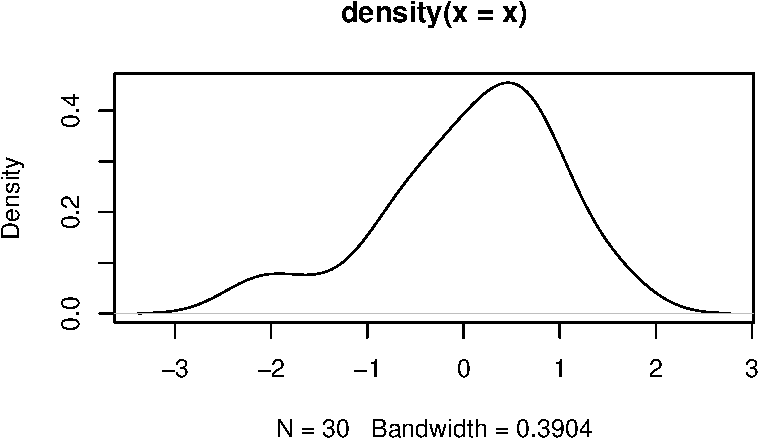
\includegraphics{04_popisna_files/figure-pdf/unnamed-chunk-4-1.pdf}

}

\end{figure}

\begin{verbatim}

-2 -1  0  1  2 
 2  5 12  9  2 

  (-2.21,-1.83]   (-1.83,-1.45]   (-1.45,-1.07]  (-1.07,-0.686] (-0.686,-0.305] 
              2               1               0               2               4 
 (-0.305,0.076]   (0.076,0.457]   (0.457,0.838]    (0.838,1.22]      (1.22,1.6] 
              5               4               7               3               2 
\end{verbatim}

\hypertarget{harmonickuxfd-prux16fmux11br}{%
\subsection{Harmonický průměr}\label{harmonickuxfd-prux16fmux11br}}

Aritmetický průměr převrácených hodnot.

\[
\bar{x_h} = \dfrac{n}{\sum\limits_{i=1}^{n}\frac{1}{x_i}}
\]

\hypertarget{prux16fmux11br-stupnux11b}{%
\subsection{\texorpdfstring{Průměr stupně
\alpha}{Průměr stupně }}\label{prux16fmux11br-stupnux11b}}

\hypertarget{annotated-cell-31}{%
\label{annotated-cell-31}}%
\begin{Shaded}
\begin{Highlighting}[]
\FunctionTok{min}\NormalTok{(x) }\CommentTok{\#\textless{}1\textgreater{}}
\FunctionTok{max}\NormalTok{(x) }\CommentTok{\#\textless{}1\textgreater{}}
\FunctionTok{max}\NormalTok{(x) }\SpecialCharTok{{-}} \FunctionTok{min}\NormalTok{(x) }\CommentTok{\#\textless{}2\textgreater{}}
\FunctionTok{range}\NormalTok{(x) }\CommentTok{\#\textless{}2\textgreater{}}
\DocumentationTok{\#\# [1] {-}2.21}
\DocumentationTok{\#\# [1] 1.6}
\DocumentationTok{\#\# [1] 3.81}
\DocumentationTok{\#\# [1] {-}2.21  1.60}
\end{Highlighting}
\end{Shaded}

\begin{description}
\tightlist
\item[\circled{1}]
Statistiky minimum \& maximum
\item[\circled{2}]
Rozpětí
\end{description}

\hypertarget{muxedry-variability}{%
\section{Míry variability}\label{muxedry-variability}}

\hypertarget{varianux10dnuxed-rozpux11btuxed}{%
\subsection{Varianční rozpětí}\label{varianux10dnuxed-rozpux11btuxed}}

Je definováno jako rozdíl \textbf{maxima} a \textbf{minima} v souboru.

\begin{Shaded}
\begin{Highlighting}[]
\FunctionTok{range}\NormalTok{(x)}
\end{Highlighting}
\end{Shaded}

\begin{verbatim}
[1] -2.21  1.60
\end{verbatim}

\hypertarget{mezikvartilovuxe9-rozpux11btuxed}{%
\subsection{Mezikvartilové
rozpětí}\label{mezikvartilovuxe9-rozpux11btuxed}}

Zatímco variační rozpětí popisuje rozpětí celého souboru, mezikvartilové
rozpětí se omezuje na rozpětí poloviny hodnot, omezené \(Q3\) a \(Q1\)
neboli \(q_{75}\) a \(q_{25}\).

\[
\mathrm{IQR} = Q3 - Q1
\]

\begin{Shaded}
\begin{Highlighting}[]
\FunctionTok{IQR}\NormalTok{(x)}
\end{Highlighting}
\end{Shaded}

\begin{verbatim}
[1] 1.1475
\end{verbatim}

\hypertarget{rozptyl}{%
\subsection{Rozptyl}\label{rozptyl}}

\[
     \sigma^2 =\sum\limits_{1}^{n}\sqrt{\dfrac{1}{n}(x_i - \bar{x})^2}
\]

\hypertarget{smux11brodatnuxe1-odchylka}{%
\subsection{Směrodatná odchylka}\label{smux11brodatnuxe1-odchylka}}

\[
   \dfrac{1}{n}\sqrt{\sum\limits_{i=1}^{n}(x_i - \bar{x})^2}
\]

Rozptyl i směrodatnou odchylku spočteme v R pomocí funkcí \texttt{var()}
(\emph{variance}) a \texttt{sd()} \emph{standard deviation}.

\begin{Shaded}
\begin{Highlighting}[]
\FunctionTok{var}\NormalTok{(x)}
\DocumentationTok{\#\# [1] 0.8537454}
\FunctionTok{sd}\NormalTok{(x)}
\DocumentationTok{\#\# [1] 0.9239834}
\end{Highlighting}
\end{Shaded}

\hypertarget{variaux10dnuxed-koeficient}{%
\subsection{Variační koeficient}\label{variaux10dnuxed-koeficient}}

\[
V = 100 \frac{s}{x}
\]

\hypertarget{stux159ednuxed-chyba-aritmetickuxe9ho-prux16fmux11bru}{%
\subsection{Střední chyba aritmetického
průměru}\label{stux159ednuxed-chyba-aritmetickuxe9ho-prux16fmux11bru}}

\[
s_x = \dfrac{s}{\sqrt{n}}
\]

\begin{tcolorbox}[enhanced jigsaw, toprule=.15mm, breakable, title=\textcolor{quarto-callout-tip-color}{\faLightbulb}\hspace{0.5em}{Cvičení}, colframe=quarto-callout-tip-color-frame, bottomrule=.15mm, left=2mm, leftrule=.75mm, colbacktitle=quarto-callout-tip-color!10!white, colback=white, bottomtitle=1mm, toptitle=1mm, opacityback=0, opacitybacktitle=0.6, arc=.35mm, coltitle=black, rightrule=.15mm, titlerule=0mm]

\begin{enumerate}
\def\labelenumi{\arabic{enumi}.}
\tightlist
\item
  Nalezněte 10\% kvantil a medián, z následujících hodnot\\
  \(0.64\), \(0.98\), \(-0.49\), \(0.75\), \(-1.35\), \(1.65\),
  \(1.12\), \(-1.04\), \(1.05\), \(0.29\), \(-0.6\), \(-0.08\),
  \(1.45\), \(-1.87\), \(-0.07\), \(-0.02\), \(0.62\), \(0.01\),
  \(-0.26\)\\
\item
  Co\\
\end{enumerate}

\end{tcolorbox}

\bookmarksetup{startatroot}

\hypertarget{sec-rozdeleni}{%
\chapter{Rozdělení pravděpodobnosti}\label{sec-rozdeleni}}

V software R jsou všechna základní rozdělení součástí balíku
\texttt{stats}. A jejich výčet získáme vyvoláním nápovědy
\texttt{?distributions}. Pracovat s rozděleními budeme čtyřmi způsoby: -
budeme generovat náhodná čísla z rozdělení - budeme pracovat s
kvantilovou funkcí daného rozdělení - počítat s hustotou a
pravděpododobnostní funkcí

Balík \texttt{stats} obsahuje mnoho rozdělení. Alternativní, Binomické,
Multinomické, Poissonov, Normální, Fischerovo, \(\chi^2\), Studentovo
\(t\) a mnohá další.

\begin{Shaded}
\begin{Highlighting}[]
\FunctionTok{r\_\_\_}\NormalTok{() }\CommentTok{\# generování náhodných čísel z rozdělení}
\FunctionTok{d\_\_\_}\NormalTok{() }\CommentTok{\# funkce hustoty rozdělení}
\FunctionTok{p\_\_\_}\NormalTok{() }\CommentTok{\# Pravděpodobnostní funkce }
\FunctionTok{q\_\_\_}\NormalTok{() }\CommentTok{\# Kvantilová funkce rozdělení}
\end{Highlighting}
\end{Shaded}

\hypertarget{distribuux10dnuxed-funkce-rozdux11blenuxed}{%
\section{Distribuční funkce
rozdělení}\label{distribuux10dnuxed-funkce-rozdux11blenuxed}}

Rozdělení pravděpodobnosti náhodné veličiny lze jednoznačně popsat tzv.
distribuční funkcí \{Rovnice~\ref{eq-distribucni-funkce}\}.

\begin{equation}\protect\hypertarget{eq-distribucni-funkce}{}{
F(x) = P(X\leq x) = P(\omega_i\in\Omega : X(\omega_i)\leq x)
}\label{eq-distribucni-funkce}\end{equation}

\hypertarget{pravdux11bpodobnostnuxed-funkce-rozdux11blenuxed}{%
\section{Pravděpodobnostní funkce
rozdělení}\label{pravdux11bpodobnostnuxed-funkce-rozdux11blenuxed}}

\hypertarget{kvantilovuxe1-funkce}{%
\section{Kvantilová funkce}\label{kvantilovuxe1-funkce}}

Kvantilová funkce je inverzní funkcí k distribuční.

\hypertarget{nuxe1hodnuxe1-ux10duxedsla}{%
\section{Náhodná čísla}\label{nuxe1hodnuxe1-ux10duxedsla}}

Pro generování náhodných čísel lze použít rozdělení.

\hypertarget{annotated-cell-36}{%
\label{annotated-cell-36}}%
\begin{Shaded}
\begin{Highlighting}[]
\FunctionTok{runif}\NormalTok{(}\AttributeTok{n =} \DecValTok{10}\NormalTok{, }\AttributeTok{min =} \DecValTok{0}\NormalTok{, }\AttributeTok{max =} \DecValTok{1}\NormalTok{) }\hspace*{\fill}\NormalTok{\circled{1}}
\FunctionTok{rpois}\NormalTok{(}\AttributeTok{n =} \DecValTok{15}\NormalTok{, }\AttributeTok{lambda =} \FloatTok{2.4}\NormalTok{) }\hspace*{\fill}\NormalTok{\circled{2}}
\end{Highlighting}
\end{Shaded}

\begin{description}
\tightlist
\item[\circled{1}]
Generování 10 čísel z rovnoměrného rozdělení z intervalu \((0;1)\)
\item[\circled{2}]
Generování 15 čísel z Poisonova rozdělení z intervalu \((0;1)\)
\end{description}

Generovaná čísla nejsou náhodná v pravém slova smyslu, ale označují se
jako \emph{pseudonáhodná}, neboť při jejich tvorbě se vychází z jiste
sekvence čísel. Tuto sekvenci je možné přímo zvolit, čímž je zajištěna

\begin{Shaded}
\begin{Highlighting}[]
\NormalTok{seed }\OtherTok{\textless{}{-}}\NormalTok{ .Random.seed}
\FunctionTok{head}\NormalTok{(seed, }\DecValTok{10}\NormalTok{)}
\end{Highlighting}
\end{Shaded}

\begin{verbatim}
 [1]       10403           2   670927727  -485657994 -1599216224   934949475
 [7] -1895927039  -951227792  -535984626  1446301305
\end{verbatim}

\begin{Shaded}
\begin{Highlighting}[]
\FunctionTok{plot}\NormalTok{(.Random.seed)}
\end{Highlighting}
\end{Shaded}

\begin{figure}[H]

{\centering 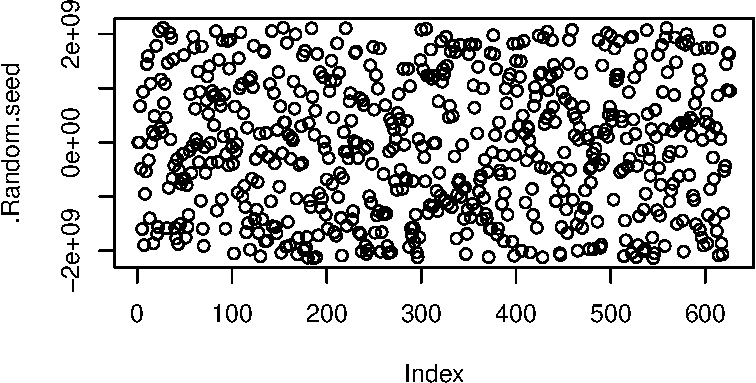
\includegraphics{05_rozdeleni_files/figure-pdf/unnamed-chunk-5-1.pdf}

}

\end{figure}

\hypertarget{annotated-cell-37}{%
\label{annotated-cell-37}}%
\begin{Shaded}
\begin{Highlighting}[]
\NormalTok{x }\OtherTok{\textless{}{-}} \FunctionTok{sample}\NormalTok{(}\AttributeTok{x =} \DecValTok{1}\SpecialCharTok{:}\FloatTok{1e3}\NormalTok{, }\AttributeTok{size =} \DecValTok{1}\NormalTok{) }\hspace*{\fill}\NormalTok{\circled{1}}
\FunctionTok{set.seed}\NormalTok{(x)  }
\FunctionTok{runif}\NormalTok{(}\DecValTok{1}\NormalTok{)}

\FunctionTok{set.seed}\NormalTok{(x)  }\hspace*{\fill}\NormalTok{\circled{2}}
\FunctionTok{runif}\NormalTok{(}\DecValTok{2}\NormalTok{)}
\end{Highlighting}
\end{Shaded}

\begin{verbatim}
[1] 0.1976203
[1] 0.1976203 0.7533784
\end{verbatim}

\hypertarget{empirickuxe9-vs.-teoretickuxe9-rozdux11blenuxed}{%
\section{Empirické vs.~teoretické
rozdělení}\label{empirickuxe9-vs.-teoretickuxe9-rozdux11blenuxed}}

\hypertarget{diskruxe9tnuxed-rozdux11blenuxed}{%
\section{Diskrétní rozdělení}\label{diskruxe9tnuxed-rozdux11blenuxed}}

\begin{Shaded}
\begin{Highlighting}[]
\NormalTok{x }\OtherTok{\textless{}{-}} \FunctionTok{rnorm}\NormalTok{(}\AttributeTok{n =} \DecValTok{10}\NormalTok{, }\AttributeTok{mean =} \FloatTok{1.25}\NormalTok{, }\AttributeTok{sd =} \FloatTok{5.36}\NormalTok{)}
\FunctionTok{mean}\NormalTok{(x)}
\end{Highlighting}
\end{Shaded}

\begin{verbatim}
[1] 0.3164631
\end{verbatim}

\begin{Shaded}
\begin{Highlighting}[]
\FunctionTok{sum}\NormalTok{(x)}
\end{Highlighting}
\end{Shaded}

\begin{verbatim}
[1] 3.164631
\end{verbatim}

\begin{Shaded}
\begin{Highlighting}[]
\FunctionTok{median}\NormalTok{(x)}
\end{Highlighting}
\end{Shaded}

\begin{verbatim}
[1] 1.086921
\end{verbatim}

\begin{Shaded}
\begin{Highlighting}[]
\FunctionTok{IQR}\NormalTok{(x)}
\end{Highlighting}
\end{Shaded}

\begin{verbatim}
[1] 5.704522
\end{verbatim}

\begin{Shaded}
\begin{Highlighting}[]
\FunctionTok{fivenum}\NormalTok{(x)}
\end{Highlighting}
\end{Shaded}

\begin{verbatim}
[1] -13.313497  -1.648298   1.086921   4.612213   9.013060
\end{verbatim}

\hypertarget{spojituxe1-rozdux11blenuxed}{%
\section{Spojitá rozdělení}\label{spojituxe1-rozdux11blenuxed}}

\begin{Shaded}
\begin{Highlighting}[]
\FunctionTok{curve}\NormalTok{(}\FunctionTok{sin}\NormalTok{(x))}
\end{Highlighting}
\end{Shaded}

\begin{figure}[H]

{\centering 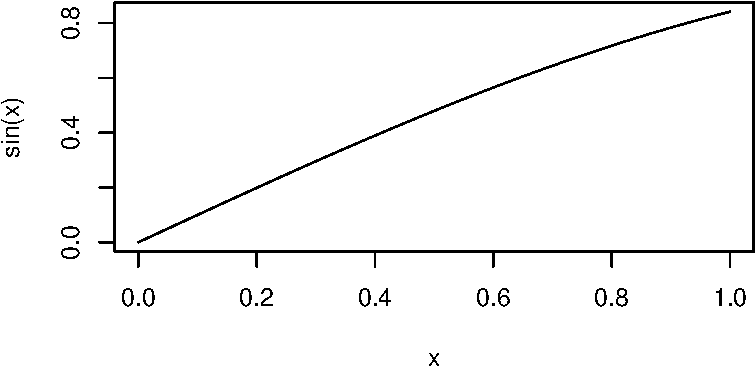
\includegraphics{05_rozdeleni_files/figure-pdf/unnamed-chunk-7-1.pdf}

}

\end{figure}

\begin{tcolorbox}[enhanced jigsaw, toprule=.15mm, breakable, title=\textcolor{quarto-callout-tip-color}{\faLightbulb}\hspace{0.5em}{Cvičení}, colframe=quarto-callout-tip-color-frame, bottomrule=.15mm, left=2mm, leftrule=.75mm, colbacktitle=quarto-callout-tip-color!10!white, colback=white, bottomtitle=1mm, toptitle=1mm, opacityback=0, opacitybacktitle=0.6, arc=.35mm, coltitle=black, rightrule=.15mm, titlerule=0mm]

\begin{enumerate}
\def\labelenumi{\arabic{enumi}.}
\tightlist
\item
  Generujte 10 čísel s pomocí normálního rozdělení s parametry
  \(\mu = 2.3\) a \(\sigma = 4.23\).
\item
  Generujte 50 čísel \(X\sim\mathsf{Po}(\lambda = 2.3)\).\\
\item
  Jaká je pravděpodobnost, že veličina \(X\sim\mathsf{N}(1.3, 4)\), bude
  nabývat hodnot menších než 6?\\
\end{enumerate}

\end{tcolorbox}

\bookmarksetup{startatroot}

\hypertarget{odhad}{%
\chapter{Bodový a intervalový odhad}\label{odhad}}

\begin{tcolorbox}[enhanced jigsaw, toprule=.15mm, breakable, title=\textcolor{quarto-callout-warning-color}{\faExclamationTriangle}\hspace{0.5em}{Cíle cvičení}, colframe=quarto-callout-warning-color-frame, bottomrule=.15mm, left=2mm, leftrule=.75mm, colbacktitle=quarto-callout-warning-color!10!white, colback=white, bottomtitle=1mm, toptitle=1mm, opacityback=0, opacitybacktitle=0.6, arc=.35mm, coltitle=black, rightrule=.15mm, titlerule=0mm]

\begin{itemize}
\tightlist
\item
  Nestrannost odhadu
\item
  Zákon velkých čísel
\item
  Bodový a intervalový odhad
\item
  \(t\)-test
\end{itemize}

\end{tcolorbox}

Obecně je odhadem v matematické statistice nazýváno určení parametru
rozdělení hodnoty určitého znaku \textbf{základního souboru} s pomocí
\textbf{výběrového souboru}.

Obecné charakteristiky základního souboru značíme písmeny řecké abecedy
(např. \(\mu\), \(\sigma\), \(\ldots\)), pro výběrové charakteristiky
volíme analogická písmena z latinky (\(\bar{x}, s_x, \ldots\)).

\hypertarget{nestrannost-odhadu}{%
\section{Nestrannost odhadu}\label{nestrannost-odhadu}}

V mnoha situacích potřebujeme odhadnout určitý parametr (střední
hodnotu, \(90\%\) kvantil atp.) neznámé náhodné veličiny. Tento parametr
odhadujeme pomocí nějaké statistiky výběru z této veličiny. Například
odhadujeme střední hodnotu veličiny pomocí průměru. Abychom mohli určit
hodnotu parametru (např. střední hodnotu) přesně, musel by být výběr
nekonečně velký. Jelikož toto v praxi nenastane, náš odhad je vždy více
či méně odlišný od skutečné hodnoty parametru (např. střední hodnoty)
neznámé veličiny. Důležitou vlastností odhadu je nestrannost - o
nestranném odhadu mluvíme pokud střední hodnota odhadu je rovna
neznámému parametru.

V přednáškách o charakteristikách náhodné veličiny a jejich odhadech je
zmíněna rovnice

\[
\dfrac{\sum\limits_{i=1}^{n}(x_i - \bar{x})^2}{n-1}
\]

jako nestranný odhad veličiny \(X\). Z definice rozptylu
\(\mathbb{E}[(X - \mathbb{E}(X^2))]\) však vyplývá odhad

\[
\dfrac{\sum\limits_{i=1}^{n}(x_i - \bar{x})^2}{n}.
\]

\begin{tcolorbox}[enhanced jigsaw, toprule=.15mm, breakable, title=\textcolor{quarto-callout-tip-color}{\faLightbulb}\hspace{0.5em}{Cvičení}, colframe=quarto-callout-tip-color-frame, bottomrule=.15mm, left=2mm, leftrule=.75mm, colbacktitle=quarto-callout-tip-color!10!white, colback=white, bottomtitle=1mm, toptitle=1mm, opacityback=0, opacitybacktitle=0.6, arc=.35mm, coltitle=black, rightrule=.15mm, titlerule=0mm]

\begin{enumerate}
\def\labelenumi{\arabic{enumi}.}
\tightlist
\item
  Doplňte následující kód.\\
\end{enumerate}

\begin{Shaded}
\begin{Highlighting}[]
\NormalTok{X }\OtherTok{\textless{}{-}} \FunctionTok{data.frame}\NormalTok{()}
\ControlFlowTok{for}\NormalTok{ (i }\ControlFlowTok{in} \DecValTok{1}\SpecialCharTok{:}\NormalTok{nsim) \{}
\NormalTok{  x }\OtherTok{\textless{}{-}} \FunctionTok{rnorm}\NormalTok{(n)}
\NormalTok{  s\_unb }\OtherTok{\textless{}{-}} \DecValTok{1}\SpecialCharTok{/}\NormalTok{(n}\DecValTok{{-}1}\NormalTok{)}
\NormalTok{  s\_bia }\OtherTok{\textless{}{-}} \DecValTok{1}\SpecialCharTok{/}\NormalTok{n}
\NormalTok{  s\_unb2 }\OtherTok{\textless{}{-}} \DecValTok{1}\SpecialCharTok{/}\NormalTok{(n}\DecValTok{{-}1}\NormalTok{)}
\NormalTok{  s\_bia2 }\OtherTok{\textless{}{-}} \DecValTok{1}\SpecialCharTok{/}\NormalTok{n}
\NormalTok{  X }\OtherTok{\textless{}{-}} \FunctionTok{rbind}\NormalTok{(X, }\FunctionTok{c}\NormalTok{(s\_unb, s\_bia, s\_unb2, s\_bia2))}
\NormalTok{\}}
\FunctionTok{names}\NormalTok{(X) }\OtherTok{=} \FunctionTok{c}\NormalTok{(}\StringTok{\textquotesingle{}UNB\textquotesingle{}}\NormalTok{, }\StringTok{\textquotesingle{}BIA\textquotesingle{}}\NormalTok{ , }\StringTok{\textquotesingle{}UNB2\textquotesingle{}}\NormalTok{ ,}\StringTok{\textquotesingle{}BIA2\textquotesingle{}}\NormalTok{)}
\end{Highlighting}
\end{Shaded}

\begin{enumerate}
\def\labelenumi{\alph{enumi})}
\tightlist
\item
  Napište funkce pro odhad ropztylu.\\
\item
  Zamyslete se, které proměnné nejsou určeny a doplňte je.\\
\item
  Spočtěte pro každou metodu průměrný odhad a systematickou chybu tohoto
  odhadu.\\
\item
  Který odhad je nejméně vychýlený a v jaké situaci?\\
\end{enumerate}

\end{tcolorbox}

\hypertarget{bodovuxfd-odhad}{%
\section{Bodový odhad}\label{bodovuxfd-odhad}}

Bodovým odhadem se se rozumí jednočíselná hodnota, která reprezentuje
vybraný moment statistického souboru jako celek. Bodovým odhadem je
například výběrový průměr nebo výběrový rozptyl.

\begin{Shaded}
\begin{Highlighting}[]
\FunctionTok{set.seed}\NormalTok{(}\DecValTok{100}\NormalTok{)}
\NormalTok{x }\OtherTok{\textless{}{-}} \FunctionTok{rnorm}\NormalTok{(}\DecValTok{10}\NormalTok{, }\DecValTok{10}\NormalTok{, }\DecValTok{10}\NormalTok{)}
\FunctionTok{mean}\NormalTok{(x)}
\DocumentationTok{\#\# [1] 9.820428}
\FunctionTok{var}\NormalTok{(x)}
\DocumentationTok{\#\# [1] 31.48541}
\end{Highlighting}
\end{Shaded}

\hypertarget{zuxe1kon-velkuxfdch-ux10duxedsel}{%
\subsection{Zákon velkých
čísel}\label{zuxe1kon-velkuxfdch-ux10duxedsel}}

Zákon velkých čísel popisuje skutečnost, že s rostoucím počtem opakování
nezávislých náhodných pokusů se empirické charakteristiky (realizované
výběrové odhady), které popisují výsledky těchto pokusů blíží k
teoretickým charakteristikám.

\begin{tcolorbox}[enhanced jigsaw, toprule=.15mm, breakable, title=\textcolor{quarto-callout-tip-color}{\faLightbulb}\hspace{0.5em}{Cvičení}, colframe=quarto-callout-tip-color-frame, bottomrule=.15mm, left=2mm, leftrule=.75mm, colbacktitle=quarto-callout-tip-color!10!white, colback=white, bottomtitle=1mm, toptitle=1mm, opacityback=0, opacitybacktitle=0.6, arc=.35mm, coltitle=black, rightrule=.15mm, titlerule=0mm]

\begin{enumerate}
\def\labelenumi{\arabic{enumi}.}
\tightlist
\item
  Generujte s pomocí funkce \texttt{rnorm} postupně \(10\), \(10^2\),
  \(10^3\), \(10^4\) čísel se shodnou střední hodnotou a shodným
  rozptylem. Spočítejte \(\bar{x}\) a \({s^2}\), použijte nápovědu.
  Okomentujte výsledky.
\end{enumerate}

\end{tcolorbox}

\hypertarget{odhad-parametru-mu-neboli-stux159ednuxed-hodnoty-normuxe1lnuxedho-rozdux11blenuxed-s-neznuxe1muxfdm-rozptylem}{%
\subsection{\texorpdfstring{Odhad parametru \(\mu\), neboli střední
hodnoty normálního rozdělení s neznámým
rozptylem}{Odhad parametru \textbackslash mu, neboli střední hodnoty normálního rozdělení s neznámým rozptylem}}\label{odhad-parametru-mu-neboli-stux159ednuxed-hodnoty-normuxe1lnuxedho-rozdux11blenuxed-s-neznuxe1muxfdm-rozptylem}}

Takto formulovaný bodový a intervalový je jednou z nejčastěji
prováděných úloh. Nejprve bodovým odhadem zjistíme \textbf{výběrový
průměr} souboru.

\begin{Shaded}
\begin{Highlighting}[]
\FunctionTok{mean}\NormalTok{(x)}
\end{Highlighting}
\end{Shaded}

\begin{verbatim}
[1] 9.820428
\end{verbatim}

Vidíme, že \(x =\) 4.9780765, 11.3153117, 9.2108291, 18.8678481,
11.1697127, 13.1863009, 4.1820932, 17.1453271, 1.7474057, 6.4013787. Pro
tento průmer následně spočítáme interval spolehlivosti.

\hypertarget{intervalovuxfd-odhad}{%
\section{Intervalový odhad}\label{intervalovuxfd-odhad}}

V případech, kdy chceme znát polohu bodového odhadu s nějakou danou
pravděpodobností, můžeme se pokusit zkonstruovat tzv.
\textbf{intervalový odhad}.

\[
\bar{X} \pm \dfrac{s}{\sqrt{n}}t_{1-\alpha/2}(n-1)
\]

\(100(1-\alpha)\%\) interval spolehlivosti je rozmezí, ve kterém se
usuzovaná hodnota základního souboru bude nacházet s určitou
pravěděpodobností.

\begin{Shaded}
\begin{Highlighting}[]
\NormalTok{alpha }\OtherTok{\textless{}{-}} \FloatTok{0.05}
\FunctionTok{cbind}\NormalTok{(}
  \FunctionTok{mean}\NormalTok{(x) }\SpecialCharTok{{-}} \FunctionTok{sd}\NormalTok{(x)}\SpecialCharTok{/}\FunctionTok{length}\NormalTok{(x)}\SpecialCharTok{*}\FunctionTok{qt}\NormalTok{(}\AttributeTok{p =} \DecValTok{1} \SpecialCharTok{{-}}\NormalTok{ alpha}\SpecialCharTok{/}\DecValTok{2}\NormalTok{, }\AttributeTok{df =} \FunctionTok{length}\NormalTok{(x) }\SpecialCharTok{{-}} \DecValTok{1}\NormalTok{),}
  \FunctionTok{mean}\NormalTok{(x) }\SpecialCharTok{+} \FunctionTok{sd}\NormalTok{(x)}\SpecialCharTok{/}\FunctionTok{length}\NormalTok{(x)}\SpecialCharTok{*}\FunctionTok{qt}\NormalTok{(}\AttributeTok{p =} \DecValTok{1} \SpecialCharTok{{-}}\NormalTok{ alpha}\SpecialCharTok{/}\DecValTok{2}\NormalTok{, }\AttributeTok{df =} \FunctionTok{length}\NormalTok{(x) }\SpecialCharTok{{-}} \DecValTok{1}\NormalTok{)}
\NormalTok{)}
\end{Highlighting}
\end{Shaded}

\begin{verbatim}
        [,1]     [,2]
[1,] 8.55109 11.08977
\end{verbatim}

\hypertarget{maximuxe1lnux11b-vux11brohodnuxfd-odhad}{%
\section{Maximálně věrohodný
odhad}\label{maximuxe1lnux11b-vux11brohodnuxfd-odhad}}

Maximálně věrohodný odhad je takový, který maximalizuje věrohodnostní
funkci \(L\) pro výběr \((x_1, x_2, \ldots, x_n)\)

\[
L(\theta, x_1, x_2, \ldots, x_n) = p(x_1, \theta) \cdot p(x_2, \theta) \cdot \ldots p(x_n, \theta) = \prod\limits_{i=1}^{n}p(x_i, \theta)
\] Konstrukce věrohodnostní funkce

\begin{Shaded}
\begin{Highlighting}[]
\CommentTok{\# Set the parameters}
\NormalTok{mean\_true }\OtherTok{\textless{}{-}} \DecValTok{5}
\NormalTok{sd\_true }\OtherTok{\textless{}{-}} \DecValTok{1}

\CommentTok{\# Generate random data from a normal distribution}
\FunctionTok{set.seed}\NormalTok{(}\DecValTok{123}\NormalTok{)}
\NormalTok{n }\OtherTok{\textless{}{-}} \DecValTok{10000}
\NormalTok{x }\OtherTok{\textless{}{-}} \FunctionTok{rnorm}\NormalTok{(n, mean\_true, sd\_true)}

\CommentTok{\# Define the likelihood function}
\NormalTok{likelihood }\OtherTok{\textless{}{-}} \ControlFlowTok{function}\NormalTok{(params) \{}
\NormalTok{  mean\_param }\OtherTok{\textless{}{-}}\NormalTok{ params[}\DecValTok{1}\NormalTok{]}
\NormalTok{  sd\_param }\OtherTok{\textless{}{-}}\NormalTok{ params[}\DecValTok{2}\NormalTok{]}
  \FunctionTok{return}\NormalTok{(}\FunctionTok{prod}\NormalTok{(}\FunctionTok{dnorm}\NormalTok{(x, }\AttributeTok{mean =}\NormalTok{ mean\_param, }\AttributeTok{sd =}\NormalTok{ sd\_param)))}
\NormalTok{\}}

\CommentTok{\# Use optim() to find the maximum likelihood estimates}
\NormalTok{result }\OtherTok{\textless{}{-}} \FunctionTok{optim}\NormalTok{(}\AttributeTok{par =} \FunctionTok{c}\NormalTok{(}\DecValTok{0}\NormalTok{, }\DecValTok{1}\NormalTok{), }\AttributeTok{fn =} \ControlFlowTok{function}\NormalTok{(params) }\SpecialCharTok{{-}}\FunctionTok{likelihood}\NormalTok{(params), }\AttributeTok{hessian =} \ConstantTok{TRUE}\NormalTok{)}

\CommentTok{\# Maximum Likelihood Estimates}
\NormalTok{mle\_mean }\OtherTok{\textless{}{-}}\NormalTok{ result}\SpecialCharTok{$}\NormalTok{par[}\DecValTok{1}\NormalTok{]}
\NormalTok{mle\_sd }\OtherTok{\textless{}{-}}\NormalTok{ result}\SpecialCharTok{$}\NormalTok{par[}\DecValTok{2}\NormalTok{]}

\FunctionTok{cat}\NormalTok{(}\StringTok{"MLE for mean:"}\NormalTok{, mle\_mean, }\StringTok{"}\SpecialCharTok{\textbackslash{}n}\StringTok{"}\NormalTok{)}
\end{Highlighting}
\end{Shaded}

\begin{verbatim}
MLE for mean: 0 
\end{verbatim}

\begin{Shaded}
\begin{Highlighting}[]
\FunctionTok{cat}\NormalTok{(}\StringTok{"MLE for standard deviation:"}\NormalTok{, mle\_sd, }\StringTok{"}\SpecialCharTok{\textbackslash{}n}\StringTok{"}\NormalTok{)}
\end{Highlighting}
\end{Shaded}

\begin{verbatim}
MLE for standard deviation: 1 
\end{verbatim}

Spočítejte hodnotu věrohodnostní funkce pro \(X = 4\)

\begin{Shaded}
\begin{Highlighting}[]
\NormalTok{n }\OtherTok{\textless{}{-}} \DecValTok{10000}
\NormalTok{x }\OtherTok{\textless{}{-}} \FunctionTok{rnorm}\NormalTok{(n, }\DecValTok{5}\NormalTok{, }\DecValTok{1}\NormalTok{)}
\NormalTok{L }\OtherTok{\textless{}{-}}\NormalTok{ x}\SpecialCharTok{*}\FunctionTok{pnorm}\NormalTok{(x, }\AttributeTok{mean =} \DecValTok{5}\NormalTok{, }\AttributeTok{sd =} \DecValTok{1}\NormalTok{)}
\FunctionTok{max}\NormalTok{(L)}
\end{Highlighting}
\end{Shaded}

\begin{verbatim}
[1] 8.757954
\end{verbatim}

\begin{Shaded}
\begin{Highlighting}[]
\FunctionTok{boxplot}\NormalTok{(x)}
\end{Highlighting}
\end{Shaded}

\begin{figure}[H]

{\centering 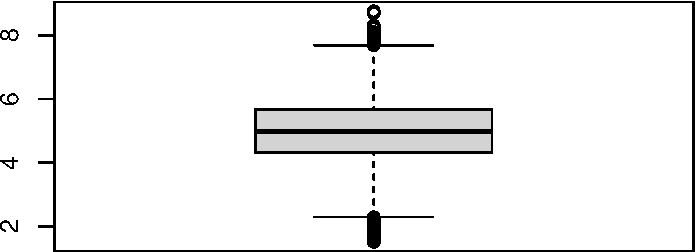
\includegraphics{06_odhad_files/figure-pdf/unnamed-chunk-6-1.pdf}

}

\end{figure}

\begin{Shaded}
\begin{Highlighting}[]
\FunctionTok{curve}\NormalTok{(}\FunctionTok{dnorm}\NormalTok{(x, }\DecValTok{4}\NormalTok{, }\DecValTok{1}\NormalTok{), }\AttributeTok{xlim =} \FunctionTok{c}\NormalTok{(}\DecValTok{0}\NormalTok{,}\DecValTok{8}\NormalTok{))}
\FunctionTok{curve}\NormalTok{(}\FunctionTok{dlnorm}\NormalTok{(x, }\DecValTok{1}\NormalTok{, }\FloatTok{0.5}\NormalTok{), }\AttributeTok{add =} \ConstantTok{TRUE}\NormalTok{)}
\end{Highlighting}
\end{Shaded}

\begin{figure}[H]

{\centering 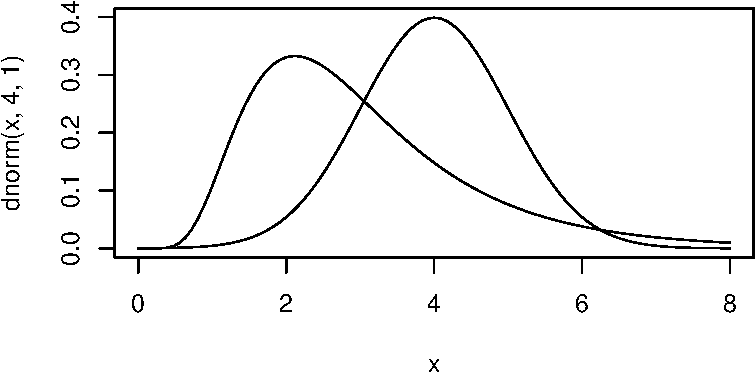
\includegraphics{06_odhad_files/figure-pdf/unnamed-chunk-6-2.pdf}

}

\end{figure}

\hypertarget{ttest}{%
\section{\texorpdfstring{\(t\)-test}{t-test}}\label{ttest}}

Nejjednodušší aplikací \(t\)-testu je Testovací statistika pro
oboustrannou alternativu má hodnotu

\[
\dfrac{|\bar{x} - \mu_0|}{s}\sqrt{n} > t_{\alpha/2}(n-1)
\] a pro jednostrannou alternativu \(\mu > \mu_0\)

\[
\dfrac{\bar{x} - \mu_0}{s}\sqrt{n} > t_{\alpha}(n-1)
\] respektive

\[
\dfrac{\bar{x} - \mu_0}{s}\sqrt{n} < t_{\alpha}(n-1)
\] pro \(\mu < \mu_0\). \(n-1\) je počet stupňů volnosti.

\begin{tcolorbox}[enhanced jigsaw, toprule=.15mm, breakable, title=\textcolor{quarto-callout-tip-color}{\faLightbulb}\hspace{0.5em}{Cvičení}, colframe=quarto-callout-tip-color-frame, bottomrule=.15mm, left=2mm, leftrule=.75mm, colbacktitle=quarto-callout-tip-color!10!white, colback=white, bottomtitle=1mm, toptitle=1mm, opacityback=0, opacitybacktitle=0.6, arc=.35mm, coltitle=black, rightrule=.15mm, titlerule=0mm]

\begin{enumerate}
\def\labelenumi{\arabic{enumi}.}
\tightlist
\item
  Spočítejte pomocí funkce \texttt{t.test} intervalový odhad pro
  \texttt{x\ =\ rnorm(100)} a \texttt{set.seed(100)}.\\
\item
  Spočítejte, zda můžeme s pravděpodobností \(90\:\%\) zamítnout
  hypotézu, že střední hodnota veličiny generující výběr
  \texttt{x\ \textless{}-\ c(0.77,\ 1.11,\ 1.14,\ 0.92,\ 0.49,\ 5.03,\ 1.35,\ 0.94,\ 0.33,\ 2.49)}
  je menší než 1.\\
\item
  Pro stejný výběr spočítejte, zda je možné na hladině významnosti
  \(0.05\) zamítnout hypotézu, že střední hodnota veličiny generující
  výběr je rovna \(1\).
\end{enumerate}

\end{tcolorbox}

\bookmarksetup{startatroot}

\hypertarget{testovuxe1nuxed-hypotuxe9z}{%
\chapter{Testování hypotéz}\label{testovuxe1nuxed-hypotuxe9z}}

\hypertarget{postup-testovuxe1nuxed-statistickuxe9-hypotuxe9zy}{%
\section{Postup testování statistické
hypotézy:}\label{postup-testovuxe1nuxed-statistickuxe9-hypotuxe9zy}}

\begin{enumerate}
\def\labelenumi{\arabic{enumi}.}
\tightlist
\item
  Formulace nulové \(H_0\) a alternativní \(H_a\) hypotézy.\\
\item
  Volba hladiny významnosti \(\alpha\).\\
\item
  Volba testovací statistiky.\\
\item
  Určení kritického oboru testové statistiky
\item
\end{enumerate}

Výsledkem testování je buď a) zamítnutní nulové hypotézy\footnote{Zamítnutí
  nulové hypotézy \textbf{neznamená, že nulová hypotéza neplatí}, ale
  znamená to, že data nevykazují objektivní důvody k jejímu přijetí} b)
nezamítnutní nulové hypotézy.

\hypertarget{p-hodnota}{%
\section{P-hodnota}\label{p-hodnota}}

Místo porovnání hodnoty testovacího kritéria s kritickými hodnotami lze
pro rozhodování o platnosti či neplatnosti nulové hypotézy použít i tzv.
\emph{p-hodnotu} (anglicky p-value). Definice p-hodnoty je poněkud
obšírná - \emph{jedná se o odhad pravděpodobnosti, že daný výsledek nebo
výsledek, který je ještě extrémnější než ten pozorovaný, mohl nastat
náhodou, za předpokladu, že nulová hypotéza je pravdivá}.

\hypertarget{alpha-interval-spolehlivosti}{%
\section{\texorpdfstring{\(100(1-\alpha)\%\) interval
spolehlivosti}{100(1-\textbackslash alpha)\textbackslash\% interval spolehlivosti}}\label{alpha-interval-spolehlivosti}}

\[
\bar{x} - 1.96\dfrac{\sigma}{\sqrt{n}}\leq\mu\leq \bar{x} + 1.96\dfrac{\sigma}{\sqrt{n}}
\]

\[
\bar{x} - t_{1-\alpha/2(\nu)}\dfrac{\sigma}{\sqrt{n}}\leq\mu\leq \bar{x} + t_{1-\alpha/2(\nu)}\dfrac{\sigma}{\sqrt{n}}
\]

kde \(\nu=n-1\) je počet stupňů volnosti.

Pravděpodobnost platnosti hypotézy

\bookmarksetup{startatroot}

\hypertarget{ux10dasovuxe9-ux159ady}{%
\chapter{Časové řady}\label{ux10dasovuxe9-ux159ady}}

Funkce pro základní statistické zpracování časových řad opět nalezneme v
balíčku \texttt{stats}, jehož jmenný prostor je připojen po otevření R.

Budeme pracovat se dvěma datovými sadami:

\begin{enumerate}
\def\labelenumi{\arabic{enumi}.}
\tightlist
\item
  Naše již připravená data z MOPEX
\item
  Vnitřní datová sada R \texttt{co2}, kterou nahrajete pomocí funkce
  \texttt{data()}
\end{enumerate}

\begin{Shaded}
\begin{Highlighting}[]
\NormalTok{dataset }\OtherTok{\textless{}{-}} \FunctionTok{readRDS}\NormalTok{(}\StringTok{"data/data.rds"}\NormalTok{)[}\DecValTok{1}\SpecialCharTok{:}\DecValTok{15000}\NormalTok{,]}
\FunctionTok{data}\NormalTok{(}\StringTok{"co2"}\NormalTok{)}
\end{Highlighting}
\end{Shaded}

\hypertarget{autokorelaux10dnuxed-funkce}{%
\section{Autokorelační funkce}\label{autokorelaux10dnuxed-funkce}}

ACF slouží k posouzení, zda časová řada obsahuje cyklickou či
periodickou složku a také, zda je či není řadou náhodnýhc čísel.
Graficky je vyjádřena pomocí korelogramu.

\begin{Shaded}
\begin{Highlighting}[]
\FunctionTok{par}\NormalTok{(}\AttributeTok{mfrow =} \FunctionTok{c}\NormalTok{(}\DecValTok{1}\NormalTok{, }\DecValTok{2}\NormalTok{))}
\FunctionTok{acf}\NormalTok{(dataset}\SpecialCharTok{$}\NormalTok{R)}
\FunctionTok{acf}\NormalTok{(co2)}
\end{Highlighting}
\end{Shaded}

\begin{figure}[H]

{\centering 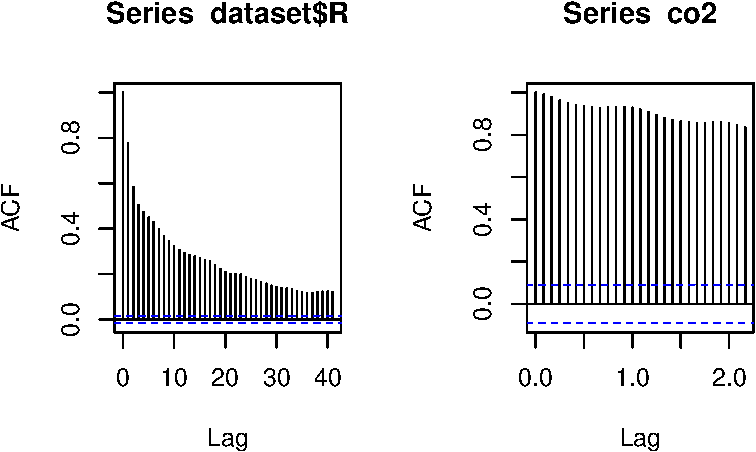
\includegraphics{09_casove_rady_files/figure-pdf/unnamed-chunk-2-1.pdf}

}

\caption{Vlevo řada se silnou autokorelací složek bez znatelené
periodicity, vpravo dtto s periodickou složkou}

\end{figure}

\hypertarget{dekompozice-ux10dasovuxe9-ux159ady}{%
\section{Dekompozice časové
řady}\label{dekompozice-ux10dasovuxe9-ux159ady}}

Dekompozicí časové řady rozumíme rozklad na složky:

\begin{enumerate}
\def\labelenumi{\arabic{enumi}.}
\tightlist
\item
  Trendovou \(T_t\)
\item
  Sezónní \(S_t\)
\item
  Cyklickou \(C_t\)
\item
  Náhodnou \(\epsilon_t\)
\end{enumerate}

\hypertarget{aditivnuxed-dekompozice}{%
\subsection{Aditivní dekompozice}\label{aditivnuxed-dekompozice}}

Předpokládáme, že řadu lze rozložit na součet složek

\[
Y_t =T_t +S_t +C_t +\epsilon_t,
\]

\begin{Shaded}
\begin{Highlighting}[]
\NormalTok{dec\_co2 }\OtherTok{\textless{}{-}} \FunctionTok{decompose}\NormalTok{(co2)}
\FunctionTok{plot}\NormalTok{(dec\_co2)}
\end{Highlighting}
\end{Shaded}

\begin{figure}[H]

{\centering 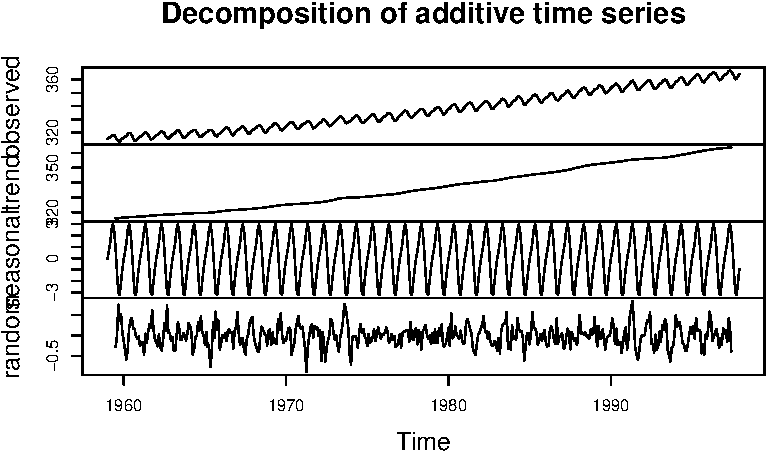
\includegraphics{09_casove_rady_files/figure-pdf/unnamed-chunk-3-1.pdf}

}

\end{figure}

\begin{Shaded}
\begin{Highlighting}[]
\FunctionTok{plot}\NormalTok{(dec\_co2}\SpecialCharTok{$}\NormalTok{trend)}
\end{Highlighting}
\end{Shaded}

\begin{figure}[H]

{\centering 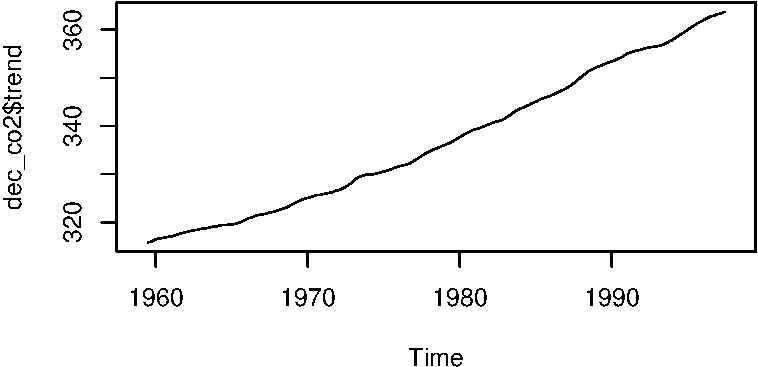
\includegraphics{09_casove_rady_files/figure-pdf/unnamed-chunk-3-2.pdf}

}

\end{figure}

\hypertarget{residua}{%
\subsection{Residua}\label{residua}}

Ověřte, zda po dekompozici \texttt{co2} residua \(\epsilon_t\) splňují
definici \emph{bílého šumu} tzn. mají nulovou střední hodnotu a konečný
rozptyl a jsou nekorelované.

\begin{Shaded}
\begin{Highlighting}[]
\FunctionTok{shapiro.test}\NormalTok{(dec\_co2}\SpecialCharTok{$}\NormalTok{random)}
\end{Highlighting}
\end{Shaded}

\begin{verbatim}

    Shapiro-Wilk normality test

data:  dec_co2$random
W = 0.99506, p-value = 0.1549
\end{verbatim}

\begin{Shaded}
\begin{Highlighting}[]
\FunctionTok{mean}\NormalTok{(dec\_co2}\SpecialCharTok{$}\NormalTok{random, }\AttributeTok{na.rm =} \ConstantTok{TRUE}\NormalTok{)}
\end{Highlighting}
\end{Shaded}

\begin{verbatim}
[1] 0.001743421
\end{verbatim}

\begin{Shaded}
\begin{Highlighting}[]
\FunctionTok{var}\NormalTok{(dec\_co2}\SpecialCharTok{$}\NormalTok{random, }\AttributeTok{na.rm =} \ConstantTok{TRUE}\NormalTok{)}
\end{Highlighting}
\end{Shaded}

\begin{verbatim}
[1] 0.07028142
\end{verbatim}

\begin{Shaded}
\begin{Highlighting}[]
\CommentTok{\# ...}
\end{Highlighting}
\end{Shaded}

\hypertarget{zhlazovacuxed-funkce}{%
\section{Zhlazovací funkce}\label{zhlazovacuxed-funkce}}

\begin{Shaded}
\begin{Highlighting}[]
\FunctionTok{par}\NormalTok{(}\AttributeTok{mfrow =} \FunctionTok{c}\NormalTok{(}\DecValTok{1}\NormalTok{, }\DecValTok{2}\NormalTok{))}
\FunctionTok{plot}\NormalTok{(dataset}\SpecialCharTok{$}\NormalTok{Tmin, }\AttributeTok{type =} \StringTok{"l"}\NormalTok{, }
     \AttributeTok{col =} \StringTok{"slategray"}\NormalTok{, }
     \AttributeTok{lwd =} \FloatTok{0.5}\NormalTok{)}
\NormalTok{md1 }\OtherTok{\textless{}{-}} \FunctionTok{loess}\NormalTok{(Tmin }\SpecialCharTok{\textasciitilde{}} \FunctionTok{na.omit}\NormalTok{(}\DecValTok{1}\SpecialCharTok{:}\FunctionTok{length}\NormalTok{(dataset}\SpecialCharTok{$}\NormalTok{Tmin)), }
             \AttributeTok{data =}\NormalTok{ dataset, }
             \AttributeTok{degree =} \DecValTok{1}\NormalTok{)}
\FunctionTok{lines}\NormalTok{(md1}\SpecialCharTok{$}\NormalTok{fitted, }\AttributeTok{col =} \StringTok{"orangered"}\NormalTok{)}

\FunctionTok{plot}\NormalTok{(}\FunctionTok{filter}\NormalTok{(}\AttributeTok{x =}\NormalTok{ dataset}\SpecialCharTok{$}\NormalTok{R, }
             \AttributeTok{method =} \StringTok{"convolution"}\NormalTok{, }
             \AttributeTok{filter =} \FunctionTok{c}\NormalTok{(}\FunctionTok{rep}\NormalTok{(}\DecValTok{1}\SpecialCharTok{/}\FloatTok{365.25}\NormalTok{, }\FloatTok{365.25}\NormalTok{)), }
             \AttributeTok{sides =} \DecValTok{1}\NormalTok{), }
      \AttributeTok{col =} \StringTok{"dodgerblue3"}\NormalTok{, }
     \AttributeTok{type =} \StringTok{"l"}\NormalTok{)}
\end{Highlighting}
\end{Shaded}

\begin{figure}[H]

{\centering 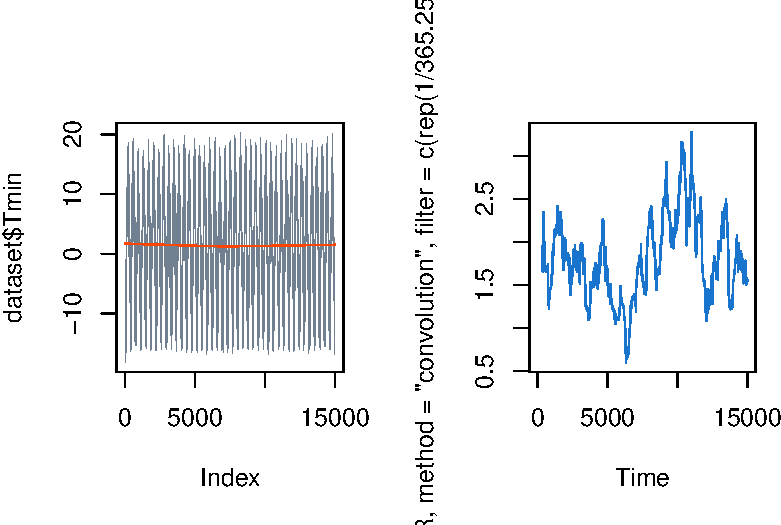
\includegraphics{09_casove_rady_files/figure-pdf/unnamed-chunk-5-1.pdf}

}

\end{figure}

\begin{Shaded}
\begin{Highlighting}[]
\NormalTok{md2 }\OtherTok{\textless{}{-}} \FunctionTok{lm}\NormalTok{(Tmin }\SpecialCharTok{\textasciitilde{}}\NormalTok{ DTM, }\AttributeTok{data =}\NormalTok{ dataset)}
\FunctionTok{plot}\NormalTok{(dataset}\SpecialCharTok{$}\NormalTok{Tmin, }\AttributeTok{type =} \StringTok{"l"}\NormalTok{, }
     \AttributeTok{col =} \StringTok{"slategray"}\NormalTok{, }
     \AttributeTok{lwd =} \FloatTok{0.5}\NormalTok{)}
\FunctionTok{lines}\NormalTok{(md1}\SpecialCharTok{$}\NormalTok{fitted, }\AttributeTok{col =} \StringTok{"darkred"}\NormalTok{)}
\FunctionTok{abline}\NormalTok{(}\FunctionTok{coef}\NormalTok{(md2), }\AttributeTok{col =} \StringTok{"orangered"}\NormalTok{)}
\end{Highlighting}
\end{Shaded}

\begin{figure}[H]

{\centering 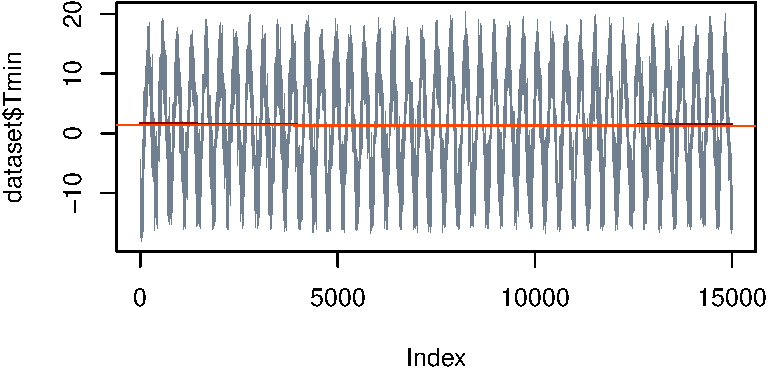
\includegraphics{09_casove_rady_files/figure-pdf/unnamed-chunk-6-1.pdf}

}

\end{figure}

\bookmarksetup{startatroot}

\hypertarget{hydroklimatickuxe9-indexy}{%
\chapter{Hydroklimatické indexy}\label{hydroklimatickuxe9-indexy}}

V software R jsou všechna základní rozdělení součástí balíku
\texttt{stats}. A jejich výčet získáme vyvoláním nápovědy
\texttt{?distributions}. Pracovat s rozděleními budeme čtyřmi způsoby: -
budeme generovat náhodná čísla z rozdělení - budeme pracovat s
kvantilovou funkcí daného rozdělení

\begin{Shaded}
\begin{Highlighting}[]
\FunctionTok{rxxx}\NormalTok{() }\CommentTok{\# náhodná čísla}
\FunctionTok{dxxx}\NormalTok{() }\CommentTok{\# }
\FunctionTok{pxxx}\NormalTok{()}
\FunctionTok{qxxx}\NormalTok{()}
\end{Highlighting}
\end{Shaded}

\hypertarget{uxfakol}{%
\subsubsection{Úkol}\label{uxfakol}}

Generujte 10 čísel s pomocí normálního rozdělení s parametry
\(\mu = 2.3\) a \(\sigma = 4.23\).

\hypertarget{diskruxe9tnuxed-rozdux11blenuxed-1}{%
\section{Diskrétní rozdělení}\label{diskruxe9tnuxed-rozdux11blenuxed-1}}

\begin{Shaded}
\begin{Highlighting}[]
\NormalTok{x }\OtherTok{\textless{}{-}} \FunctionTok{rnorm}\NormalTok{(}\AttributeTok{n =} \DecValTok{10}\NormalTok{, }\AttributeTok{mean =} \FloatTok{1.25}\NormalTok{, }\AttributeTok{sd =} \FloatTok{5.36}\NormalTok{)}
\FunctionTok{mean}\NormalTok{(x)}
\end{Highlighting}
\end{Shaded}

\begin{verbatim}
[1] 1.420126
\end{verbatim}

\begin{Shaded}
\begin{Highlighting}[]
\FunctionTok{sum}\NormalTok{(x)}
\end{Highlighting}
\end{Shaded}

\begin{verbatim}
[1] 14.20126
\end{verbatim}

\begin{Shaded}
\begin{Highlighting}[]
\FunctionTok{median}\NormalTok{(x)}
\end{Highlighting}
\end{Shaded}

\begin{verbatim}
[1] 1.13559
\end{verbatim}

\begin{Shaded}
\begin{Highlighting}[]
\FunctionTok{IQR}\NormalTok{(x)}
\end{Highlighting}
\end{Shaded}

\begin{verbatim}
[1] 6.796219
\end{verbatim}

\begin{Shaded}
\begin{Highlighting}[]
\FunctionTok{fivenum}\NormalTok{(x)}
\end{Highlighting}
\end{Shaded}

\begin{verbatim}
[1] -4.770726 -1.758516  1.135590  6.028678  8.327783
\end{verbatim}

\hypertarget{spojituxe1-rozdux11blenuxed-1}{%
\section{Spojitá rozdělení}\label{spojituxe1-rozdux11blenuxed-1}}

\begin{Shaded}
\begin{Highlighting}[]
\FunctionTok{curve}\NormalTok{(}\FunctionTok{sin}\NormalTok{(x))}
\end{Highlighting}
\end{Shaded}

\begin{figure}[H]

{\centering 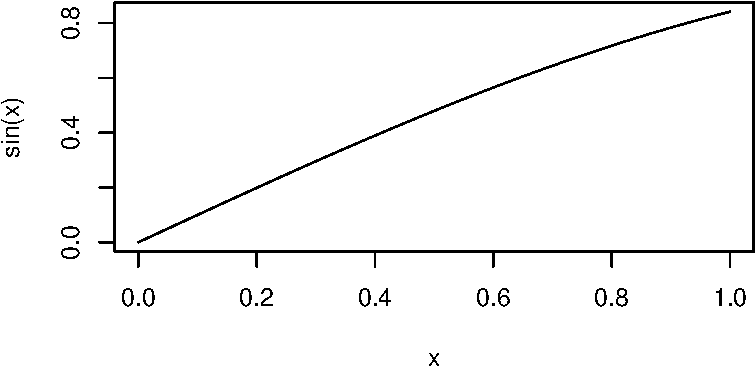
\includegraphics{10_hydro_index_files/figure-pdf/unnamed-chunk-3-1.pdf}

}

\end{figure}

\bookmarksetup{startatroot}

\hypertarget{seq-zavislost}{%
\chapter{Závislost dvou veličin}\label{seq-zavislost}}

\hypertarget{sec-korelace}{%
\section{Korelace}\label{sec-korelace}}

Korelace je vztah mezi dvěma náhodnými veličinami. Zkoumá, zda se jedna
ze zkoumaných veličin mění, pokud se zároveň mění i druhá.Korelace
nezkoumá příčinnost, nelze tedy jednoznačně určit závislou a nezávislou
proměnnou.

Míru korelace dvou veličin posuzujeme korelačním koeficientem. V případe
normality u obou veličin lze použít \textbf{Paersonův} korelační
koeficient,

\begin{equation}\protect\hypertarget{eq-pearson}{}{
r_{xy} = \dfrac{\sum(x_i - \bar{x})(y_i - \bar{y})}{\sqrt{\sum(x_i - \bar{x})^2}\sqrt{\sum(y_i - \bar{y})^2}}
}\label{eq-pearson}\end{equation}

přičemž platí \(r_{xy}\in\langle-1;1\rangle\). Alternativně můžeme
použít neparametrický výpočet \textbf{Spearmana}, založený na
diferencích pořadí pozorovaných hodnot, které definujeme jako
\(d_i = x_{ri} - y_{ri}\)

\begin{equation}\protect\hypertarget{eq-spearman}{}{
\rho = r_s = 1 - \dfrac{6\sum_{i=1}^{n}d_i^2}{n(n^2-1)} 
}\label{eq-spearman}\end{equation}

\begin{tcolorbox}[enhanced jigsaw, toprule=.15mm, breakable, title=\textcolor{quarto-callout-tip-color}{\faLightbulb}\hspace{0.5em}{Cvičení}, colframe=quarto-callout-tip-color-frame, bottomrule=.15mm, left=2mm, leftrule=.75mm, colbacktitle=quarto-callout-tip-color!10!white, colback=white, bottomtitle=1mm, toptitle=1mm, opacityback=0, opacitybacktitle=0.6, arc=.35mm, coltitle=black, rightrule=.15mm, titlerule=0mm]

\begin{enumerate}
\def\labelenumi{\arabic{enumi}.}
\tightlist
\item
  Napište vlastní funkci, které pro dané vektory \texttt{x} a \texttt{y}
  spočítá korelační Spearmanův koeficient.\\
\end{enumerate}

\begin{enumerate}
\def\labelenumi{\alph{enumi})}
\tightlist
\item
  Nejprve je nutné identifikovat pořadí,\\
\item
  dále spočítat kvadrát vzdáleností,\\
\item
  a po dosazení počtu měření \(n\) dosadit do rovnice.\\
\end{enumerate}

\begin{enumerate}
\def\labelenumi{\arabic{enumi}.}
\setcounter{enumi}{1}
\tightlist
\item
  Vyzkoušejte obě funkce na datech
\end{enumerate}

Řešení:\\

\begin{Shaded}
\begin{Highlighting}[]
\NormalTok{sp\_k }\OtherTok{\textless{}{-}} \ControlFlowTok{function}\NormalTok{(x, y) \{}
\NormalTok{  rank\_x }\OtherTok{\textless{}{-}} \FunctionTok{rank}\NormalTok{(x) }
\NormalTok{  rank\_y }\OtherTok{\textless{}{-}} \FunctionTok{rank}\NormalTok{(y) }
\NormalTok{  d }\OtherTok{\textless{}{-}}\NormalTok{ rank\_x }\SpecialCharTok{{-}}\NormalTok{ rank\_y }
\NormalTok{  d\_sq }\OtherTok{\textless{}{-}} \FunctionTok{sum}\NormalTok{(d}\SpecialCharTok{\^{}}\DecValTok{2}\NormalTok{) }
\NormalTok{  n }\OtherTok{\textless{}{-}} \FunctionTok{length}\NormalTok{(x) }
  \DecValTok{1} \SpecialCharTok{{-}}\NormalTok{ ((}\DecValTok{6} \SpecialCharTok{*}\NormalTok{ d\_sq) }\SpecialCharTok{/}\NormalTok{ (n}\SpecialCharTok{*}\NormalTok{(n}\SpecialCharTok{\^{}}\DecValTok{2} \SpecialCharTok{{-}} \DecValTok{1}\NormalTok{))) }
\NormalTok{\}}
\end{Highlighting}
\end{Shaded}

\begin{Shaded}
\begin{Highlighting}[]
\FunctionTok{sp\_k}\NormalTok{(\_, \_)}
\FunctionTok{cor}\NormalTok{(\_, \_, }\AttributeTok{method =} \StringTok{"Spearman"}\NormalTok{)}
\end{Highlighting}
\end{Shaded}

\begin{enumerate}
\def\labelenumi{\arabic{enumi}.}
\setcounter{enumi}{2}
\tightlist
\item
  Pokuste se odhadnout korelační koeficient následujících veličin
\end{enumerate}

\begin{figure}[H]

{\centering 
\includegraphics{11_korelace_regrese_files/figure-pdf/unnamed-chunk-3-1.pdf}

}

\end{figure}

\end{tcolorbox}

\hypertarget{regrese}{%
\section{Regrese}\label{regrese}}

Narozdíl od korelace, v regresní analýze sledujeme příčinnou závislost.
Identifikujeme \textbf{nezávislou proměnnou} a \textbf{závislou
proměnnou}. Míru závislosti posuzujeme pomocí lineárního regresního
modelu. Cílem regrese je proložit naměřenými body přímku, která nejlépe
vystihuje vztah mezi proměnnými.

\[
y = \beta_0 + \beta_1x
\] kde \(y\) je závislá proměnná, \(x\) je nezávislá proměnná,
\(\beta_0\) je počátek (intercept) a \(\beta_1\) je sklon přímky.

Lineární model regresního typu definujeme v R pomocí funkce
\texttt{lm()}, které na první pozici dosazujeme výraz ve formátu rovnice
\texttt{formula}, např. \texttt{lm(y\ \textasciitilde{}\ x)}. Model
vyhodnocujeme funkcí \texttt{summary} a mezi sebou porovnáváme pomocí
kritérií zohledňující vysvětlenou variabilitu/věrohodnost modelu a jeho
komplexnost, např. \textbf{Akaikeho informační kritérium}.

\[
\text{AIC} = 2k - 2\ln(\hat{L})
\] kde \(k\) je počet volných parametrů modelu a \(\hat{L}\) je
věrohodnostní funkce modelu.

\hypertarget{cviux10denuxed-8}{%
\paragraph*{Cvičení}\label{cviux10denuxed-8}}
\addcontentsline{toc}{paragraph}{Cvičení}

\begin{enumerate}
\def\labelenumi{\arabic{enumi}.}
\tightlist
\item
  Uvažujme následující data, kde předpokládáme příčinnou závislost \(y\)
  na \(x\).
\end{enumerate}

\begin{Shaded}
\begin{Highlighting}[]
\NormalTok{dfr }\OtherTok{\textless{}{-}} \FunctionTok{data.frame}\NormalTok{(}
\NormalTok{  x }\OtherTok{\textless{}{-}} \FunctionTok{c}\NormalTok{( }\FloatTok{3.93}\NormalTok{,  }\FloatTok{3.83}\NormalTok{,  }\FloatTok{7.11}\NormalTok{,  }\FloatTok{6.98}\NormalTok{,  }\FloatTok{7.87}\NormalTok{,  }\FloatTok{9.11}\NormalTok{, }\FloatTok{10.04}\NormalTok{,  }\FloatTok{9.99}\NormalTok{, }\FloatTok{10.11}\NormalTok{, }\FloatTok{10.93}\NormalTok{, }
         \FloatTok{11.01}\NormalTok{, }\FloatTok{11.93}\NormalTok{, }\FloatTok{11.94}\NormalTok{, }\FloatTok{11.88}\NormalTok{, }\FloatTok{11.82}\NormalTok{, }\FloatTok{12.98}\NormalTok{, }\FloatTok{13.04}\NormalTok{, }\FloatTok{13.04}\NormalTok{, }\FloatTok{13.11}\NormalTok{, }\FloatTok{13.99}\NormalTok{, }
         \FloatTok{13.97}\NormalTok{, }\FloatTok{13.99}\NormalTok{, }\FloatTok{13.97}\NormalTok{, }\FloatTok{15.08}\NormalTok{, }\FloatTok{14.93}\NormalTok{, }\FloatTok{14.86}\NormalTok{, }\FloatTok{15.89}\NormalTok{, }\FloatTok{16.15}\NormalTok{, }\FloatTok{17.08}\NormalTok{, }\FloatTok{17.18}\NormalTok{, }
         \FloatTok{16.96}\NormalTok{, }\FloatTok{17.95}\NormalTok{, }\FloatTok{18.14}\NormalTok{, }\FloatTok{18.09}\NormalTok{, }\FloatTok{18.05}\NormalTok{, }\FloatTok{19.04}\NormalTok{, }\FloatTok{19.08}\NormalTok{, }\FloatTok{19.07}\NormalTok{, }\FloatTok{20.11}\NormalTok{, }\DecValTok{20}\NormalTok{, }
         \DecValTok{20}\NormalTok{,    }\FloatTok{20.14}\NormalTok{, }\FloatTok{19.92}\NormalTok{, }\FloatTok{22.13}\NormalTok{, }\FloatTok{23.09}\NormalTok{, }\FloatTok{23.9}\NormalTok{ , }\FloatTok{23.95}\NormalTok{, }\FloatTok{24.06}\NormalTok{, }\FloatTok{23.95}\NormalTok{, }\FloatTok{24.94}
\NormalTok{  ),}
\NormalTok{  y }\OtherTok{\textless{}{-}} \FunctionTok{c}\NormalTok{( }\FloatTok{1.93}\NormalTok{, }\FloatTok{10.01}\NormalTok{,  }\FloatTok{3.73}\NormalTok{, }\FloatTok{22.09}\NormalTok{, }\FloatTok{15.86}\NormalTok{, }\FloatTok{10.09}\NormalTok{, }\FloatTok{18.09}\NormalTok{, }\FloatTok{25.91}\NormalTok{, }\FloatTok{34.09}\NormalTok{, }\FloatTok{16.89}\NormalTok{, }
         \FloatTok{28.04}\NormalTok{, }\FloatTok{13.95}\NormalTok{, }\FloatTok{19.98}\NormalTok{, }\FloatTok{23.98}\NormalTok{, }\FloatTok{27.78}\NormalTok{, }\FloatTok{26.19}\NormalTok{, }\FloatTok{33.85}\NormalTok{, }\FloatTok{33.96}\NormalTok{, }\FloatTok{45.88}\NormalTok{, }\FloatTok{25.96}\NormalTok{, }
         \FloatTok{35.89}\NormalTok{, }\FloatTok{60.}\NormalTok{  , }\FloatTok{80.03}\NormalTok{, }\FloatTok{20.06}\NormalTok{, }\FloatTok{25.92}\NormalTok{, }\FloatTok{54.03}\NormalTok{, }\FloatTok{31.96}\NormalTok{, }\FloatTok{40.12}\NormalTok{, }\FloatTok{32.03}\NormalTok{, }\FloatTok{39.95}\NormalTok{, }
         \FloatTok{50.2}\NormalTok{ , }\FloatTok{41.91}\NormalTok{, }\FloatTok{55.92}\NormalTok{, }\FloatTok{75.92}\NormalTok{, }\FloatTok{83.89}\NormalTok{, }\FloatTok{35.94}\NormalTok{, }\FloatTok{45.94}\NormalTok{, }\FloatTok{67.85}\NormalTok{, }\FloatTok{32.05}\NormalTok{, }\FloatTok{48.11}\NormalTok{, }
         \FloatTok{52.11}\NormalTok{, }\FloatTok{55.95}\NormalTok{, }\FloatTok{64.02}\NormalTok{, }\FloatTok{65.9}\NormalTok{ , }\FloatTok{53.94}\NormalTok{, }\FloatTok{69.92}\NormalTok{, }\FloatTok{92.1}\NormalTok{ , }\FloatTok{92.78}\NormalTok{, }\FloatTok{99.03}\NormalTok{, }\FloatTok{85.09}\NormalTok{)}
\NormalTok{)}
\end{Highlighting}
\end{Shaded}

\begin{enumerate}
\def\labelenumi{\arabic{enumi}.}
\setcounter{enumi}{1}
\tightlist
\item
  Sestrojme lineární model \texttt{md1}
\end{enumerate}

\begin{Shaded}
\begin{Highlighting}[]
\NormalTok{md1 }\OtherTok{\textless{}{-}} \FunctionTok{lm}\NormalTok{(}\AttributeTok{formula =}\NormalTok{ y }\SpecialCharTok{\textasciitilde{}}\NormalTok{ x, }\AttributeTok{data =}\NormalTok{ dfr)}
\end{Highlighting}
\end{Shaded}

\begin{enumerate}
\def\labelenumi{\arabic{enumi}.}
\setcounter{enumi}{2}
\tightlist
\item
  Struktura objektu \texttt{md1} je komplexní, můžeme vybírat jednotlivé
  proměnné k dalším účelům, například pro tvorbu grafů.
\end{enumerate}

\begin{Shaded}
\begin{Highlighting}[]
\FunctionTok{str}\NormalTok{(md1, }\DecValTok{1}\NormalTok{)}
\end{Highlighting}
\end{Shaded}

\begin{verbatim}
List of 12
 $ coefficients : Named num [1:2] -15.72 3.78
  ..- attr(*, "names")= chr [1:2] "(Intercept)" "x"
 $ residuals    : Named num [1:50] 2.79 11.25 -7.43 11.42 1.82 ...
  ..- attr(*, "names")= chr [1:50] "1" "2" "3" "4" ...
 $ effects      : Named num [1:50] -300.7778 140.5186 -9.3636 9.458 0.0675 ...
  ..- attr(*, "names")= chr [1:50] "(Intercept)" "x" "" "" ...
 $ rank         : int 2
 $ fitted.values: Named num [1:50] -0.862 -1.24 11.163 10.672 14.037 ...
  ..- attr(*, "names")= chr [1:50] "1" "2" "3" "4" ...
 $ assign       : int [1:2] 0 1
 $ qr           :List of 5
  ..- attr(*, "class")= chr "qr"
 $ df.residual  : int 48
 $ xlevels      : Named list()
 $ call         : language lm(formula = y ~ x, data = dfr)
 $ terms        :Classes 'terms', 'formula'  language y ~ x
  .. ..- attr(*, "variables")= language list(y, x)
  .. ..- attr(*, "factors")= int [1:2, 1] 0 1
  .. .. ..- attr(*, "dimnames")=List of 2
  .. ..- attr(*, "term.labels")= chr "x"
  .. ..- attr(*, "order")= int 1
  .. ..- attr(*, "intercept")= int 1
  .. ..- attr(*, "response")= int 1
  .. ..- attr(*, ".Environment")=<environment: R_GlobalEnv> 
  .. ..- attr(*, "predvars")= language list(y, x)
  .. ..- attr(*, "dataClasses")= Named chr [1:2] "numeric" "numeric"
  .. .. ..- attr(*, "names")= chr [1:2] "y" "x"
 $ model        :'data.frame':  50 obs. of  2 variables:
  ..- attr(*, "terms")=Classes 'terms', 'formula'  language y ~ x
  .. .. ..- attr(*, "variables")= language list(y, x)
  .. .. ..- attr(*, "factors")= int [1:2, 1] 0 1
  .. .. .. ..- attr(*, "dimnames")=List of 2
  .. .. ..- attr(*, "term.labels")= chr "x"
  .. .. ..- attr(*, "order")= int 1
  .. .. ..- attr(*, "intercept")= int 1
  .. .. ..- attr(*, "response")= int 1
  .. .. ..- attr(*, ".Environment")=<environment: R_GlobalEnv> 
  .. .. ..- attr(*, "predvars")= language list(y, x)
  .. .. ..- attr(*, "dataClasses")= Named chr [1:2] "numeric" "numeric"
  .. .. .. ..- attr(*, "names")= chr [1:2] "y" "x"
 - attr(*, "class")= chr "lm"
\end{verbatim}

\begin{Shaded}
\begin{Highlighting}[]
\FunctionTok{with}\NormalTok{(}\AttributeTok{data =}\NormalTok{ dfr, }
     \AttributeTok{expr =} \FunctionTok{plot}\NormalTok{(x, }
\NormalTok{                 y, }
                 \AttributeTok{xlim =} \FunctionTok{c}\NormalTok{(}\DecValTok{0}\NormalTok{, }\DecValTok{30}\NormalTok{), }
                 \AttributeTok{ylim =} \FunctionTok{c}\NormalTok{(md1}\SpecialCharTok{$}\NormalTok{coefficients[}\DecValTok{1}\NormalTok{], }
                          \FunctionTok{max}\NormalTok{(md1}\SpecialCharTok{$}\NormalTok{fitted.values) }\SpecialCharTok{+} \DecValTok{2}\NormalTok{)))}
\FunctionTok{abline}\NormalTok{(md1}\SpecialCharTok{$}\NormalTok{coefficients, }\AttributeTok{col =} \StringTok{"orangered"}\NormalTok{)}
\FunctionTok{abline}\NormalTok{(}\AttributeTok{v =} \DecValTok{0}\NormalTok{, }\AttributeTok{lty =} \StringTok{"dashed"}\NormalTok{)}
\FunctionTok{abline}\NormalTok{(}\AttributeTok{h =}\NormalTok{ md1}\SpecialCharTok{$}\NormalTok{coefficients[}\DecValTok{1}\NormalTok{], }\AttributeTok{lty =} \StringTok{"dashed"}\NormalTok{)}
\end{Highlighting}
\end{Shaded}

\begin{figure}[H]

{\centering \includegraphics{11_korelace_regrese_files/figure-pdf/unnamed-chunk-7-1.pdf}

}

\end{figure}

\begin{enumerate}
\def\labelenumi{\arabic{enumi}.}
\setcounter{enumi}{3}
\tightlist
\item
  Model vyhodnotíme pomocí \texttt{summary}
\end{enumerate}

\begin{Shaded}
\begin{Highlighting}[]
\FunctionTok{summary}\NormalTok{(md1)}
\end{Highlighting}
\end{Shaded}

\begin{verbatim}

Call:
lm(formula = y ~ x, data = dfr)

Residuals:
    Min      1Q  Median      3Q     Max 
-28.274  -9.410  -1.639  10.063  42.925 

Coefficients:
            Estimate Std. Error t value Pr(>|t|)    
(Intercept) -15.7241     6.3224  -2.487   0.0164 *  
x             3.7816     0.3884   9.736 6.03e-13 ***
---
Signif. codes:  0 '***' 0.001 '**' 0.01 '*' 0.05 '.' 0.1 ' ' 1

Residual standard error: 14.43 on 48 degrees of freedom
Multiple R-squared:  0.6639,    Adjusted R-squared:  0.6568 
F-statistic: 94.79 on 1 and 48 DF,  p-value: 6.032e-13
\end{verbatim}

Souhrn obsahuje původní zadání v podobě rovnice, dále identifikované
koeficienty modelu, významnost závislosti indikuje přítomnost jedné nebo
více \texttt{*} u vysvětlující proměnné; dále lze vyčíst podíl
vysvětlené variabiltiy \texttt{Adjusted\ R-squared:\ \ 0.6417}.\\

\begin{Shaded}
\begin{Highlighting}[]
\FunctionTok{par}\NormalTok{(}\AttributeTok{mfrow =} \FunctionTok{c}\NormalTok{(}\DecValTok{2}\NormalTok{, }\DecValTok{2}\NormalTok{))}
\FunctionTok{plot}\NormalTok{(md1, }\DecValTok{1}\SpecialCharTok{:}\DecValTok{4}\NormalTok{)}
\end{Highlighting}
\end{Shaded}

\begin{figure}[H]

{\centering \includegraphics{11_korelace_regrese_files/figure-pdf/unnamed-chunk-9-1.pdf}

}

\end{figure}

R dále poskytuje grafické nástroje k posouzení vhodnosti zvoleného
modelu. Zde nás budou zajímat zejména \textbf{residua} modelu. Dle
prvního grafu by mohl model se závislostí na polynomu být lepší
volbou.\\

Pokusme se sestavit alternativní model s kvadratickou vysvětlující
proměnnou.

\begin{Shaded}
\begin{Highlighting}[]
\NormalTok{md2 }\OtherTok{\textless{}{-}} \FunctionTok{lm}\NormalTok{(y }\SpecialCharTok{\textasciitilde{}} \FunctionTok{poly}\NormalTok{(x, }\DecValTok{2}\NormalTok{))}
\FunctionTok{summary}\NormalTok{(md2)}
\end{Highlighting}
\end{Shaded}

\begin{verbatim}

Call:
lm(formula = y ~ poly(x, 2))

Residuals:
    Min      1Q  Median      3Q     Max 
-28.086  -9.010  -3.459   4.693  45.048 

Coefficients:
            Estimate Std. Error t value Pr(>|t|)    
(Intercept)   42.536      2.027  20.985  < 2e-16 ***
poly(x, 2)1  140.519     14.333   9.804 6.05e-13 ***
poly(x, 2)2   18.519     14.333   1.292    0.203    
---
Signif. codes:  0 '***' 0.001 '**' 0.01 '*' 0.05 '.' 0.1 ' ' 1

Residual standard error: 14.33 on 47 degrees of freedom
Multiple R-squared:  0.6754,    Adjusted R-squared:  0.6616 
F-statistic: 48.89 on 2 and 47 DF,  p-value: 3.29e-12
\end{verbatim}

\begin{Shaded}
\begin{Highlighting}[]
\FunctionTok{par}\NormalTok{(}\AttributeTok{mfrow =} \FunctionTok{c}\NormalTok{(}\DecValTok{2}\NormalTok{, }\DecValTok{2}\NormalTok{))}
\FunctionTok{plot}\NormalTok{(md2, }\DecValTok{1}\SpecialCharTok{:}\DecValTok{4}\NormalTok{)}
\end{Highlighting}
\end{Shaded}

\begin{figure}[H]

{\centering \includegraphics{11_korelace_regrese_files/figure-pdf/unnamed-chunk-11-1.pdf}

}

\end{figure}

\begin{Shaded}
\begin{Highlighting}[]
\FunctionTok{with}\NormalTok{(}\AttributeTok{data =}\NormalTok{ dfr, }
     \AttributeTok{expr =} \FunctionTok{plot}\NormalTok{(x, y, }\AttributeTok{xlim =} \FunctionTok{c}\NormalTok{(}\DecValTok{0}\NormalTok{, }\DecValTok{30}\NormalTok{)))}
\NormalTok{pred }\OtherTok{\textless{}{-}} \FunctionTok{predict}\NormalTok{(md2)}
\NormalTok{ix }\OtherTok{\textless{}{-}} \FunctionTok{sort}\NormalTok{(dfr}\SpecialCharTok{$}\NormalTok{x, }\AttributeTok{index.return=}\NormalTok{T)}\SpecialCharTok{$}\NormalTok{ix}
\FunctionTok{lines}\NormalTok{(x[ix], pred[ix], }\AttributeTok{col =} \StringTok{\textquotesingle{}orangered\textquotesingle{}}\NormalTok{)}
\end{Highlighting}
\end{Shaded}

\begin{figure}[H]

{\centering \includegraphics{11_korelace_regrese_files/figure-pdf/unnamed-chunk-12-1.pdf}

}

\end{figure}

Srovnejme modely vzájemně

\begin{Shaded}
\begin{Highlighting}[]
\FunctionTok{AIC}\NormalTok{(md1, md2)}
\end{Highlighting}
\end{Shaded}

\begin{verbatim}
    df      AIC
md1  3 412.8013
md2  4 413.0561
\end{verbatim}

\begin{tcolorbox}[enhanced jigsaw, toprule=.15mm, breakable, title=\textcolor{quarto-callout-tip-color}{\faLightbulb}\hspace{0.5em}{Cvičení}, colframe=quarto-callout-tip-color-frame, bottomrule=.15mm, left=2mm, leftrule=.75mm, colbacktitle=quarto-callout-tip-color!10!white, colback=white, bottomtitle=1mm, toptitle=1mm, opacityback=0, opacitybacktitle=0.6, arc=.35mm, coltitle=black, rightrule=.15mm, titlerule=0mm]

\begin{enumerate}
\def\labelenumi{\arabic{enumi}.}
\tightlist
\item
  Prozkoumejte závislost odtoku na velikosti povodí~
\end{enumerate}

\begin{longtable}[]{@{}
  >{\raggedright\arraybackslash}p{(\columnwidth - 12\tabcolsep) * \real{0.1053}}
  >{\raggedright\arraybackslash}p{(\columnwidth - 12\tabcolsep) * \real{0.2105}}
  >{\raggedright\arraybackslash}p{(\columnwidth - 12\tabcolsep) * \real{0.1053}}
  >{\raggedright\arraybackslash}p{(\columnwidth - 12\tabcolsep) * \real{0.1711}}
  >{\raggedright\arraybackslash}p{(\columnwidth - 12\tabcolsep) * \real{0.1053}}
  >{\raggedright\arraybackslash}p{(\columnwidth - 12\tabcolsep) * \real{0.1842}}
  >{\raggedright\arraybackslash}p{(\columnwidth - 12\tabcolsep) * \real{0.1184}}@{}}
\toprule\noalign{}
\begin{minipage}[b]{\linewidth}\raggedright
Povodí
\end{minipage} & \begin{minipage}[b]{\linewidth}\raggedright
velikost \(x_i\)
\end{minipage} & \begin{minipage}[b]{\linewidth}\raggedright
pořadí
\end{minipage} & \begin{minipage}[b]{\linewidth}\raggedright
odtok \(y_i\)
\end{minipage} & \begin{minipage}[b]{\linewidth}\raggedright
pořadí
\end{minipage} & \begin{minipage}[b]{\linewidth}\raggedright
rozdíl \(d_i\)
\end{minipage} & \begin{minipage}[b]{\linewidth}\raggedright
\(d_i^2\)
\end{minipage} \\
\midrule\noalign{}
\endhead
\bottomrule\noalign{}
\endlastfoot
1 & & & & & & \\
2 & & & & & & \\
3 & & & & & & \\
4 & & & & & & \\
5 & & & & & & \\
6 & & & & & & \\
7 & & & & & & \\
8 & & & & & & \\
9 & & & & & & \\
10 & & & & & & \\
\end{longtable}

\end{tcolorbox}

\bookmarksetup{startatroot}

\hypertarget{extremuxe1lnuxed-rozdux11blenuxed}{%
\chapter{Extremální rozdělení}\label{extremuxe1lnuxed-rozdux11blenuxed}}

\hypertarget{weibullovo-rozdux11blenuxed}{%
\section{Weibullovo rozdělení}\label{weibullovo-rozdux11blenuxed}}

Korelace je vztah mezi dvěma náhodnými veličinami. Zkoumá, zda se jedna
ze zkoumaných veličin mění, pokud se zároveň mění i druhá.Korelace
nezkoumá příčinnost, nelze tedy jednoznačně určit závislou a nezávislou
proměnnou.

Míru korelace dvou veličin posuzujeme korelačním koeficientem. V případe
normality u obou veličin lze použít \textbf{Paersonův} korelační
koeficient,

\[
r_{xy} = \dfrac{\sum(x_i - \bar{x})(y_i - \bar{y})}{\sqrt{\sum(x_i - \bar{x})^2}\sqrt{\sum(y_i - \bar{y})^2}}
\] přičemž platí \(r_{xy}\in\langle-1;1\rangle\). Alternativně můžeme
použít neparametrický výpočet \textbf{Spearmana}, založený na
diferencích pořadí pozorovaných hodnot, které definujeme jako
\(d_i = x_{ri} - y_{ri}\)

\begin{equation}\protect\hypertarget{eq-spearman}{}{
\rho = r_s = 1 - \dfrac{6\sum_{i=1}^{n}d_i^2}{n(n^2-1)} 
}\label{eq-spearman}\end{equation}

\hypertarget{cviux10denuxed-10}{%
\subsubsection*{Cvičení}\label{cviux10denuxed-10}}
\addcontentsline{toc}{subsubsection}{Cvičení}

\begin{itemize}
\tightlist
\item
  Napište vlastní funkci, které pro dané vektory \texttt{x} a \texttt{y}
  spočítá korelační Spearmanův koeficient.\\
  Řešení:
\end{itemize}

\hypertarget{annotated-cell-81}{%
\label{annotated-cell-81}}%
\begin{Shaded}
\begin{Highlighting}[]
\NormalTok{sp\_k }\OtherTok{\textless{}{-}} \ControlFlowTok{function}\NormalTok{(x, y) \{}
\NormalTok{  rank\_x }\OtherTok{\textless{}{-}} \FunctionTok{rank}\NormalTok{(x) }\hspace*{\fill}\NormalTok{\circled{1}}
\NormalTok{  rank\_y }\OtherTok{\textless{}{-}} \FunctionTok{rank}\NormalTok{(y) }
\NormalTok{  d }\OtherTok{\textless{}{-}}\NormalTok{ rank\_x }\SpecialCharTok{{-}}\NormalTok{ rank\_y }\hspace*{\fill}\NormalTok{\circled{2}}
\NormalTok{  d\_sq }\OtherTok{\textless{}{-}} \FunctionTok{sum}\NormalTok{(d}\SpecialCharTok{\^{}}\DecValTok{2}\NormalTok{) }
\NormalTok{  n }\OtherTok{\textless{}{-}} \FunctionTok{length}\NormalTok{(x) }\hspace*{\fill}\NormalTok{\circled{3}}
  
  \DecValTok{1} \SpecialCharTok{{-}}\NormalTok{ ((}\DecValTok{6} \SpecialCharTok{*}\NormalTok{ d\_sq) }\SpecialCharTok{/}\NormalTok{ (n}\SpecialCharTok{*}\NormalTok{(n}\SpecialCharTok{\^{}}\DecValTok{2} \SpecialCharTok{{-}} \DecValTok{1}\NormalTok{))) }
  
\NormalTok{\}}
\end{Highlighting}
\end{Shaded}

\begin{description}
\tightlist
\item[\circled{1}]
Nejprve je nutné identifikovat pořadí,
\item[\circled{2}]
dále spočítat kvadrát vzdáleností,
\item[\circled{3}]
a po dosazení počtu měření \(n\) dosadit do rovnice.
\end{description}

\begin{itemize}
\tightlist
\item
  Porovnejte obě funkce na datech
\end{itemize}

\begin{Shaded}
\begin{Highlighting}[]
\FunctionTok{sp\_k}\NormalTok{(\_, \_)}
\FunctionTok{cor}\NormalTok{(\_, \_, }\AttributeTok{method =} \StringTok{"Spearman"}\NormalTok{)}
\end{Highlighting}
\end{Shaded}

\begin{itemize}
\tightlist
\item
  Pokuste se odhadnout korelační koeficient následujících veličin
\end{itemize}


\includegraphics{12_extremalni_rozdeleni_files/figure-pdf/unnamed-chunk-3-1.pdf}

\begin{longtable}[]{@{}
  >{\raggedright\arraybackslash}p{(\columnwidth - 12\tabcolsep) * \real{0.1053}}
  >{\raggedright\arraybackslash}p{(\columnwidth - 12\tabcolsep) * \real{0.2105}}
  >{\raggedright\arraybackslash}p{(\columnwidth - 12\tabcolsep) * \real{0.1053}}
  >{\raggedright\arraybackslash}p{(\columnwidth - 12\tabcolsep) * \real{0.1711}}
  >{\raggedright\arraybackslash}p{(\columnwidth - 12\tabcolsep) * \real{0.1053}}
  >{\raggedright\arraybackslash}p{(\columnwidth - 12\tabcolsep) * \real{0.1842}}
  >{\raggedright\arraybackslash}p{(\columnwidth - 12\tabcolsep) * \real{0.1184}}@{}}
\toprule\noalign{}
\begin{minipage}[b]{\linewidth}\raggedright
Povodí
\end{minipage} & \begin{minipage}[b]{\linewidth}\raggedright
velikost \(x_i\)
\end{minipage} & \begin{minipage}[b]{\linewidth}\raggedright
pořadí
\end{minipage} & \begin{minipage}[b]{\linewidth}\raggedright
odtok \(y_i\)
\end{minipage} & \begin{minipage}[b]{\linewidth}\raggedright
pořadí
\end{minipage} & \begin{minipage}[b]{\linewidth}\raggedright
rozdíl \(d_i\)
\end{minipage} & \begin{minipage}[b]{\linewidth}\raggedright
\(d_i^2\)
\end{minipage} \\
\midrule\noalign{}
\endhead
\bottomrule\noalign{}
\endlastfoot
1 & & & & & & \\
2 & & & & & & \\
3 & & & & & & \\
4 & & & & & & \\
5 & & & & & & \\
6 & & & & & & \\
7 & & & & & & \\
8 & & & & & & \\
9 & & & & & & \\
10 & & & & & & \\
\end{longtable}

\hypertarget{regrese-1}{%
\section{Regrese}\label{regrese-1}}

Narozdíl od korelace, v regresní analýze sledujeme příčinnou závislost.
Identifikujeme \textbf{nezávislou proměnnou} a \textbf{závislou
proměnnou}. Míru závislosti posuzujeme pomocí lineárního regresního
modelu. Cílem regrese je proložit naměřenými body přímku, která nejlépe
vystihuje vztah mezi proměnnými.

\[
y = \beta_0 + \beta_1x
\] kde \(y\) je závislá proměnná, \(x\) je nezávislá proměnná,
\(\beta_0\) je počátek (intercept) a \(\beta_1\) je sklon přímky.

Lineární model regresního typu definujeme v R pomocí funkce
\texttt{lm()}, které na první pozici dosazujeme výraz ve formátu rovnice
\texttt{formula}, např. \texttt{lm(y\ \textasciitilde{}\ x)}. Model
vyhodnocujeme funkcí \texttt{summary} a mezi sebou porovnáváme pomocí
kritérií zohledňující vysvětlenou variabilitu/věrohodnost modelu a jeho
komplexnost, např. \textbf{Akaikeho informační kritérium}.

\[
\text{AIC} = 2k - 2\ln(\hat{L})
\] kde \(k\) je počet volných parametrů modelu a \(\hat{L}\) je
věrohodnostní funkce modelu.

\hypertarget{cviux10denuxed-11}{%
\paragraph*{Cvičení}\label{cviux10denuxed-11}}
\addcontentsline{toc}{paragraph}{Cvičení}

\begin{enumerate}
\def\labelenumi{\arabic{enumi}.}
\tightlist
\item
  Uvažujme následující data, kde předpokládáme příčinnou závislost \(y\)
  na \(x\).
\end{enumerate}

\begin{Shaded}
\begin{Highlighting}[]
\NormalTok{dfr }\OtherTok{\textless{}{-}} \FunctionTok{data.frame}\NormalTok{(}
\NormalTok{  x }\OtherTok{\textless{}{-}} \FunctionTok{c}\NormalTok{( }\FloatTok{3.93}\NormalTok{,  }\FloatTok{3.83}\NormalTok{,  }\FloatTok{7.11}\NormalTok{,  }\FloatTok{6.98}\NormalTok{,  }\FloatTok{7.87}\NormalTok{,  }\FloatTok{9.11}\NormalTok{, }\FloatTok{10.04}\NormalTok{,  }\FloatTok{9.99}\NormalTok{, }\FloatTok{10.11}\NormalTok{, }\FloatTok{10.93}\NormalTok{, }
         \FloatTok{11.01}\NormalTok{, }\FloatTok{11.93}\NormalTok{, }\FloatTok{11.94}\NormalTok{, }\FloatTok{11.88}\NormalTok{, }\FloatTok{11.82}\NormalTok{, }\FloatTok{12.98}\NormalTok{, }\FloatTok{13.04}\NormalTok{, }\FloatTok{13.04}\NormalTok{, }\FloatTok{13.11}\NormalTok{, }\FloatTok{13.99}\NormalTok{, }
         \FloatTok{13.97}\NormalTok{, }\FloatTok{13.99}\NormalTok{, }\FloatTok{13.97}\NormalTok{, }\FloatTok{15.08}\NormalTok{, }\FloatTok{14.93}\NormalTok{, }\FloatTok{14.86}\NormalTok{, }\FloatTok{15.89}\NormalTok{, }\FloatTok{16.15}\NormalTok{, }\FloatTok{17.08}\NormalTok{, }\FloatTok{17.18}\NormalTok{, }
         \FloatTok{16.96}\NormalTok{, }\FloatTok{17.95}\NormalTok{, }\FloatTok{18.14}\NormalTok{, }\FloatTok{18.09}\NormalTok{, }\FloatTok{18.05}\NormalTok{, }\FloatTok{19.04}\NormalTok{, }\FloatTok{19.08}\NormalTok{, }\FloatTok{19.07}\NormalTok{, }\FloatTok{20.11}\NormalTok{, }\DecValTok{20}\NormalTok{, }
         \DecValTok{20}\NormalTok{,    }\FloatTok{20.14}\NormalTok{, }\FloatTok{19.92}\NormalTok{, }\FloatTok{22.13}\NormalTok{, }\FloatTok{23.09}\NormalTok{, }\FloatTok{23.9}\NormalTok{ , }\FloatTok{23.95}\NormalTok{, }\FloatTok{24.06}\NormalTok{, }\FloatTok{23.95}\NormalTok{, }\FloatTok{24.94}
\NormalTok{  ),}
\NormalTok{  y }\OtherTok{\textless{}{-}} \FunctionTok{c}\NormalTok{( }\FloatTok{1.93}\NormalTok{, }\FloatTok{10.01}\NormalTok{,  }\FloatTok{3.73}\NormalTok{, }\FloatTok{22.09}\NormalTok{, }\FloatTok{15.86}\NormalTok{, }\FloatTok{10.09}\NormalTok{, }\FloatTok{18.09}\NormalTok{, }\FloatTok{25.91}\NormalTok{, }\FloatTok{34.09}\NormalTok{, }\FloatTok{16.89}\NormalTok{, }
         \FloatTok{28.04}\NormalTok{, }\FloatTok{13.95}\NormalTok{, }\FloatTok{19.98}\NormalTok{, }\FloatTok{23.98}\NormalTok{, }\FloatTok{27.78}\NormalTok{, }\FloatTok{26.19}\NormalTok{, }\FloatTok{33.85}\NormalTok{, }\FloatTok{33.96}\NormalTok{, }\FloatTok{45.88}\NormalTok{, }\FloatTok{25.96}\NormalTok{, }
         \FloatTok{35.89}\NormalTok{, }\FloatTok{60.}\NormalTok{  , }\FloatTok{80.03}\NormalTok{, }\FloatTok{20.06}\NormalTok{, }\FloatTok{25.92}\NormalTok{, }\FloatTok{54.03}\NormalTok{, }\FloatTok{31.96}\NormalTok{, }\FloatTok{40.12}\NormalTok{, }\FloatTok{32.03}\NormalTok{, }\FloatTok{39.95}\NormalTok{, }
         \FloatTok{50.2}\NormalTok{ , }\FloatTok{41.91}\NormalTok{, }\FloatTok{55.92}\NormalTok{, }\FloatTok{75.92}\NormalTok{, }\FloatTok{83.89}\NormalTok{, }\FloatTok{35.94}\NormalTok{, }\FloatTok{45.94}\NormalTok{, }\FloatTok{67.85}\NormalTok{, }\FloatTok{32.05}\NormalTok{, }\FloatTok{48.11}\NormalTok{, }
         \FloatTok{52.11}\NormalTok{, }\FloatTok{55.95}\NormalTok{, }\FloatTok{64.02}\NormalTok{, }\FloatTok{65.9}\NormalTok{ , }\FloatTok{53.94}\NormalTok{, }\FloatTok{69.92}\NormalTok{, }\FloatTok{92.1}\NormalTok{ , }\FloatTok{92.78}\NormalTok{, }\FloatTok{99.03}\NormalTok{, }\FloatTok{85.09}\NormalTok{)}
\NormalTok{)}
\end{Highlighting}
\end{Shaded}

\begin{enumerate}
\def\labelenumi{\arabic{enumi}.}
\setcounter{enumi}{1}
\tightlist
\item
  Sestrojme lineární model \texttt{md1}
\end{enumerate}

\begin{Shaded}
\begin{Highlighting}[]
\NormalTok{md1 }\OtherTok{\textless{}{-}} \FunctionTok{lm}\NormalTok{(}\AttributeTok{formula =}\NormalTok{ y }\SpecialCharTok{\textasciitilde{}}\NormalTok{ x, }\AttributeTok{data =}\NormalTok{ dfr)}
\end{Highlighting}
\end{Shaded}

\begin{enumerate}
\def\labelenumi{\arabic{enumi}.}
\setcounter{enumi}{2}
\tightlist
\item
  Struktura objektu \texttt{md1} je komplexní, můžeme vybírat jednotlivé
  proměnné k dalším účelům, například pro tvorbu grafů.
\end{enumerate}

\begin{Shaded}
\begin{Highlighting}[]
\FunctionTok{str}\NormalTok{(md1, }\DecValTok{1}\NormalTok{)}
\end{Highlighting}
\end{Shaded}

\begin{verbatim}
List of 12
 $ coefficients : Named num [1:2] -15.72 3.78
  ..- attr(*, "names")= chr [1:2] "(Intercept)" "x"
 $ residuals    : Named num [1:50] 2.79 11.25 -7.43 11.42 1.82 ...
  ..- attr(*, "names")= chr [1:50] "1" "2" "3" "4" ...
 $ effects      : Named num [1:50] -300.7778 140.5186 -9.3636 9.458 0.0675 ...
  ..- attr(*, "names")= chr [1:50] "(Intercept)" "x" "" "" ...
 $ rank         : int 2
 $ fitted.values: Named num [1:50] -0.862 -1.24 11.163 10.672 14.037 ...
  ..- attr(*, "names")= chr [1:50] "1" "2" "3" "4" ...
 $ assign       : int [1:2] 0 1
 $ qr           :List of 5
  ..- attr(*, "class")= chr "qr"
 $ df.residual  : int 48
 $ xlevels      : Named list()
 $ call         : language lm(formula = y ~ x, data = dfr)
 $ terms        :Classes 'terms', 'formula'  language y ~ x
  .. ..- attr(*, "variables")= language list(y, x)
  .. ..- attr(*, "factors")= int [1:2, 1] 0 1
  .. .. ..- attr(*, "dimnames")=List of 2
  .. ..- attr(*, "term.labels")= chr "x"
  .. ..- attr(*, "order")= int 1
  .. ..- attr(*, "intercept")= int 1
  .. ..- attr(*, "response")= int 1
  .. ..- attr(*, ".Environment")=<environment: R_GlobalEnv> 
  .. ..- attr(*, "predvars")= language list(y, x)
  .. ..- attr(*, "dataClasses")= Named chr [1:2] "numeric" "numeric"
  .. .. ..- attr(*, "names")= chr [1:2] "y" "x"
 $ model        :'data.frame':  50 obs. of  2 variables:
  ..- attr(*, "terms")=Classes 'terms', 'formula'  language y ~ x
  .. .. ..- attr(*, "variables")= language list(y, x)
  .. .. ..- attr(*, "factors")= int [1:2, 1] 0 1
  .. .. .. ..- attr(*, "dimnames")=List of 2
  .. .. ..- attr(*, "term.labels")= chr "x"
  .. .. ..- attr(*, "order")= int 1
  .. .. ..- attr(*, "intercept")= int 1
  .. .. ..- attr(*, "response")= int 1
  .. .. ..- attr(*, ".Environment")=<environment: R_GlobalEnv> 
  .. .. ..- attr(*, "predvars")= language list(y, x)
  .. .. ..- attr(*, "dataClasses")= Named chr [1:2] "numeric" "numeric"
  .. .. .. ..- attr(*, "names")= chr [1:2] "y" "x"
 - attr(*, "class")= chr "lm"
\end{verbatim}

\begin{Shaded}
\begin{Highlighting}[]
\FunctionTok{with}\NormalTok{(}\AttributeTok{data =}\NormalTok{ dfr, }
     \AttributeTok{expr =} \FunctionTok{plot}\NormalTok{(x, }
\NormalTok{                 y, }
                 \AttributeTok{xlim =} \FunctionTok{c}\NormalTok{(}\DecValTok{0}\NormalTok{, }\DecValTok{30}\NormalTok{), }
                 \AttributeTok{ylim =} \FunctionTok{c}\NormalTok{(md1}\SpecialCharTok{$}\NormalTok{coefficients[}\DecValTok{1}\NormalTok{], }
                          \FunctionTok{max}\NormalTok{(md1}\SpecialCharTok{$}\NormalTok{fitted.values) }\SpecialCharTok{+} \DecValTok{2}\NormalTok{)))}
\FunctionTok{abline}\NormalTok{(md1}\SpecialCharTok{$}\NormalTok{coefficients, }\AttributeTok{col =} \StringTok{"orangered"}\NormalTok{)}
\FunctionTok{abline}\NormalTok{(}\AttributeTok{v =} \DecValTok{0}\NormalTok{, }\AttributeTok{lty =} \StringTok{"dashed"}\NormalTok{)}
\FunctionTok{abline}\NormalTok{(}\AttributeTok{h =}\NormalTok{ md1}\SpecialCharTok{$}\NormalTok{coefficients[}\DecValTok{1}\NormalTok{], }\AttributeTok{lty =} \StringTok{"dashed"}\NormalTok{)}
\end{Highlighting}
\end{Shaded}

\begin{figure}[H]

{\centering \includegraphics{12_extremalni_rozdeleni_files/figure-pdf/unnamed-chunk-7-1.pdf}

}

\end{figure}

\begin{enumerate}
\def\labelenumi{\arabic{enumi}.}
\setcounter{enumi}{3}
\tightlist
\item
  Model vyhodnotíme pomocí \texttt{summary}
\end{enumerate}

\begin{Shaded}
\begin{Highlighting}[]
\FunctionTok{summary}\NormalTok{(md1)}
\end{Highlighting}
\end{Shaded}

\begin{verbatim}

Call:
lm(formula = y ~ x, data = dfr)

Residuals:
    Min      1Q  Median      3Q     Max 
-28.274  -9.410  -1.639  10.063  42.925 

Coefficients:
            Estimate Std. Error t value Pr(>|t|)    
(Intercept) -15.7241     6.3224  -2.487   0.0164 *  
x             3.7816     0.3884   9.736 6.03e-13 ***
---
Signif. codes:  0 '***' 0.001 '**' 0.01 '*' 0.05 '.' 0.1 ' ' 1

Residual standard error: 14.43 on 48 degrees of freedom
Multiple R-squared:  0.6639,    Adjusted R-squared:  0.6568 
F-statistic: 94.79 on 1 and 48 DF,  p-value: 6.032e-13
\end{verbatim}

Souhrn obsahuje původní zadání v podobě rovnice, dále identifikované
koeficienty modelu, významnost závislosti indikuje přítomnost jedné nebo
více \texttt{*} u vysvětlující proměnné; dále lze vyčíst podíl
vysvětlené variabiltiy \texttt{Adjusted\ R-squared:\ \ 0.6417}.\\

\begin{Shaded}
\begin{Highlighting}[]
\FunctionTok{par}\NormalTok{(}\AttributeTok{mfrow =} \FunctionTok{c}\NormalTok{(}\DecValTok{2}\NormalTok{, }\DecValTok{2}\NormalTok{))}
\FunctionTok{plot}\NormalTok{(md1, }\DecValTok{1}\SpecialCharTok{:}\DecValTok{4}\NormalTok{)}
\end{Highlighting}
\end{Shaded}

\begin{figure}[H]

{\centering \includegraphics{12_extremalni_rozdeleni_files/figure-pdf/unnamed-chunk-9-1.pdf}

}

\end{figure}

R dále poskytuje grafické nástroje k posouzení vhodnosti zvoleného
modelu. Zde nás budou zajímat zejména \textbf{residua} modelu. Dle
prvního grafu by mohl model se závislostí na polynomu být lepší
volbou.\\

Pokusme se sestavit alternativní model s kvadratickou vysvětlující
proměnnou.

\begin{Shaded}
\begin{Highlighting}[]
\NormalTok{md2 }\OtherTok{\textless{}{-}} \FunctionTok{lm}\NormalTok{(y }\SpecialCharTok{\textasciitilde{}} \FunctionTok{poly}\NormalTok{(x, }\DecValTok{2}\NormalTok{))}
\FunctionTok{summary}\NormalTok{(md2)}
\end{Highlighting}
\end{Shaded}

\begin{verbatim}

Call:
lm(formula = y ~ poly(x, 2))

Residuals:
    Min      1Q  Median      3Q     Max 
-28.086  -9.010  -3.459   4.693  45.048 

Coefficients:
            Estimate Std. Error t value Pr(>|t|)    
(Intercept)   42.536      2.027  20.985  < 2e-16 ***
poly(x, 2)1  140.519     14.333   9.804 6.05e-13 ***
poly(x, 2)2   18.519     14.333   1.292    0.203    
---
Signif. codes:  0 '***' 0.001 '**' 0.01 '*' 0.05 '.' 0.1 ' ' 1

Residual standard error: 14.33 on 47 degrees of freedom
Multiple R-squared:  0.6754,    Adjusted R-squared:  0.6616 
F-statistic: 48.89 on 2 and 47 DF,  p-value: 3.29e-12
\end{verbatim}

\begin{Shaded}
\begin{Highlighting}[]
\FunctionTok{par}\NormalTok{(}\AttributeTok{mfrow =} \FunctionTok{c}\NormalTok{(}\DecValTok{2}\NormalTok{, }\DecValTok{2}\NormalTok{))}
\FunctionTok{plot}\NormalTok{(md2, }\DecValTok{1}\SpecialCharTok{:}\DecValTok{4}\NormalTok{)}
\end{Highlighting}
\end{Shaded}

\begin{figure}[H]

{\centering \includegraphics{12_extremalni_rozdeleni_files/figure-pdf/unnamed-chunk-11-1.pdf}

}

\end{figure}

\begin{Shaded}
\begin{Highlighting}[]
\FunctionTok{with}\NormalTok{(}\AttributeTok{data =}\NormalTok{ dfr, }
     \AttributeTok{expr =} \FunctionTok{plot}\NormalTok{(x, y, }\AttributeTok{xlim =} \FunctionTok{c}\NormalTok{(}\DecValTok{0}\NormalTok{, }\DecValTok{30}\NormalTok{)))}
\NormalTok{pred }\OtherTok{\textless{}{-}} \FunctionTok{predict}\NormalTok{(md2)}
\NormalTok{ix }\OtherTok{\textless{}{-}} \FunctionTok{sort}\NormalTok{(dfr}\SpecialCharTok{$}\NormalTok{x, }\AttributeTok{index.return=}\NormalTok{T)}\SpecialCharTok{$}\NormalTok{ix}
\FunctionTok{lines}\NormalTok{(x[ix], pred[ix], }\AttributeTok{col =} \StringTok{\textquotesingle{}orangered\textquotesingle{}}\NormalTok{)}
\end{Highlighting}
\end{Shaded}

\begin{figure}[H]

{\centering \includegraphics{12_extremalni_rozdeleni_files/figure-pdf/unnamed-chunk-12-1.pdf}

}

\end{figure}

Srovnejme modely vzájemně

\begin{Shaded}
\begin{Highlighting}[]
\FunctionTok{AIC}\NormalTok{(md1, md2)}
\end{Highlighting}
\end{Shaded}

\begin{verbatim}
    df      AIC
md1  3 412.8013
md2  4 413.0561
\end{verbatim}

\begin{itemize}
\tightlist
\item
  Pokuste se vést diskuzi nad vhodností obou modelů
\end{itemize}

\hypertarget{refs}{}
\begin{CSLReferences}{1}{0}
\leavevmode\vadjust pre{\hypertarget{ref-jaruskova2006}{}}%
Jarušková, Daniela. 2006. \emph{Pravděpodobnost a matematická
statistika}. Česká technika-nakladatelství ČVUT.

\leavevmode\vadjust pre{\hypertarget{ref-pus2007}{}}%
Puš, Vladimír. 2007. \emph{Popisná statistika}. Česká zemědělská
univerizita v Praze.

\end{CSLReferences}



\end{document}
